\documentclass[
    %draft, % Mit % kommentieren, um Bilder sichtbar zu machen und Links zu aktivieren
    pdftex,
    a4paper,
    twoside,
    parskip,
    numbers=noenddot,
    listof=totoc,
    bibliography=totoc,
    hyperfootnotes=false,
    english,
    openright
]{scrreprt}
\setuptoc{toc}{totoc}

\newcommand{\thesistitle}{Identification of key information with topic analysis on large unstructured text data}
\newcommand{\thesistype}{B A C H E L O R  T H E S I S}
\newcommand{\thesistypedesc}{Department of Electrical Engineering and Computer Science \\
    University of Kassel}
\newcommand{\thesisauthorname}{Klara Maximiliane Gutekunst}
\newcommand{\thesisauthorhomestreet}{*** REMOVED ***}
\newcommand{\thesisauthorhometown}{34125 Kassel}
\newcommand{\thesisauthormatrikelnumber}{*** REMOVED ***}
\newcommand{\thesisauthoremail}{klara.gutekunst@student.uni-kassel.de}
\newcommand{\thesisdepartment}{Chair Intelligent Embedded Systems}
\newcommand{\thesisfirstreviewer}{Prof.\ Dr.\ rer.\ nat.\ Bernhard Sick}
\newcommand{\thesissecondreviewer}{Prof.\ Dr.\ Gerd Stumme}
\newcommand{\thesissupervisor}{Dr.\ Christian Gruhl}
\newcommand{\thesisdate}{\today}
\newcommand{\eigenfaces}{Eigenfaces}
\newcommand{\eigendocs}{Eigendocs}

% Select input encoding, usually utf8 is the best choice, on windows, \usepackage[latin1]{inputenc} maybe required
\usepackage[utf8]{inputenc}
\usepackage[T1]{fontenc}
\usepackage[english]{babel}
\usepackage{csquotes}
\usepackage{xcolor}

\MakeOuterQuote{"} % Damit ist es möglich, " " zu verwenden ohne Umlaut zu erzeugen
\defaulthyphenchar=127 % Dadurch werden auch Wörter mit Bindestrich getrennt, die schon Bindestriche enthalten.

% geometry
\usepackage[bindingoffset=1cm, left=2.5cm, right=2.5cm, top=2.5cm, bottom=2.5cm]{geometry}

% Headline
\usepackage{fancyhdr}
\pagestyle{fancy}
\renewcommand{\chaptermark}[1]{\markboth{\thechapter\ #1}{}}
\lhead{\leftmark} \rhead{\thepage}
\cfoot{}
\fancypagestyle{plain}{}

\RedeclareSectionCommand[beforeskip=1.5cm,afterskip=1cm]{chapter}

% Colors
\usepackage{color}
\usepackage{colortbl}

% Tables
\usepackage{tabularx}
\usepackage{multirow}
\setlength{\tabcolsep}{4pt}

% Drawing graphs etc.
\usepackage{pgf}
\usepackage{tikz}
\usetikzlibrary{arrows,automata}

% Footnotes
\usepackage{footmisc}
\usepackage{xspace}
\newcommand{\sic}{[\acs{sic}]\xspace}

% math
\usepackage{amsmath}
\usepackage{amssymb}

\usepackage{siunitx}

% lists
\usepackage{paralist}

% Figures
\usepackage{graphicx, wrapfig}

% Hyperlinks
\usepackage[hyphens]{url}
\usepackage{hyperref}
\hypersetup{colorlinks, citecolor=black, linkcolor=black, urlcolor=black}

% Minted
\usepackage[chapter]{minted}
%\usemintedstyle{xcode}
\setminted{frame=single,tabsize=2,linenos,autogobble}

\newmintinline[code]{text}{breaklines}

\newminted[mdcodeblock]{md}{autogobble,frame=none,linenos=false,breaklines}

% list of abbreviations
\usepackage[printonlyused]{acronym}

% Set line pitch
\usepackage{setspace}
\onehalfspacing              % anderthalbzeilig (oder auch \doublespace)

%fancyBox
%\usepackage{fancybox}

% Layout corrections (Schusterjungen)
\clubpenalty = 10000
% Layout corrections (Hurenkinder)
\widowpenalty = 10000
\displaywidowpenalty = 10000

% Figures
\usepackage{caption}
\usepackage[hypcap=true,labelformat=simple]{subcaption}
\renewcommand{\thesubfigure}{(\alph{subfigure})}
\usepackage[inkscapelatex=false]{svg}

% Tables
\usepackage{booktabs}
%\usepackage[table,xcdraw]{xcolor}

% enumerate
\usepackage{enumitem}

% Bibliography
\usepackage[square,numbers]{natbib}
\bibliographystyle{plainnat} % or plainnat abbrvnat unsrtnat

% Frequently used column types
\newcolumntype{C}[1]{>{\centering\arraybackslash}p{#1}} % centering column type with fixed width
\newcolumntype{R}[1]{>{\raggedleft\arraybackslash}p{#1}} % right aligned column type with fixed width
\newcolumntype{L}[1]{>{\raggedright\arraybackslash}p{#1}} % left aligned column type with fixed width

% Shortcuts for referencing floats:
\newcommand{\fig}[1]{\figurename~\ref{#1}} %shortcut for a figure reference
\newcommand{\tab}[1]{Table~\ref{#1}} %shortcut for a table reference
\newcommand{\eq}[1]{(\ref{#1})} %shortcut for an equation reference
\newcommand{\lst}[1]{Listing~\ref{#1}} %shortcut for a listing reference
\newcommand{\sect}[1]{Section~\ref{#1}} %shortcut for a Section reference

% Shortcut for terms
\newcommand{\databaseName}{Elasticsearch}



\begin{document}

    \pagenumbering{roman}

    \begin{titlepage}
	% Select font without serifs
	\sffamily

	% Logo
	\begin{tabularx}{\textwidth}{@{}l@{}>{\raggedleft\arraybackslash}X@{}r@{}}
		\multirow{2}{*}{
\includegraphics[width=6.8cm]{images/Logo_UniKassel}} &
		\raisebox{-1mm}{\small{Department of Electrical Engineering and Computer Science}} \\
		&\raisebox{-1mm}{\small{\thesisdepartment}} &
	\end{tabularx}

	\vspace{2.5cm}

	\begin{center}
		% Title and subtitle
		\huge{\thesistitle}

		\vspace{3cm}

		\renewcommand{\baselinestretch}{1.3}
		\Large{\thesistype}

		\large
		\thesistypedesc
	\end{center}

	\vspace{1.5cm}
	\renewcommand{\baselinestretch}{1}
	\begin{table}[htpb]
		\centering
		\begin{tabular}{ll}
			\\
			Author Name: & \thesisauthorname \\
			Address: & \thesisauthorhomestreet \\
			& \thesisauthorhometown \\
			\\
			Matriculation number: & \thesisauthormatrikelnumber \\
			E-Mail: & \thesisauthoremail \\
			\\
			Department: & \thesisdepartment \\
			\\
			Examining board 1: & \thesisfirstreviewer \\
			Examining board 2: & \thesissecondreviewer \\
			\\
			Supervisor: & \thesissupervisor \\
			\\
			Date: & \thesisdate \\
		\end{tabular}
	\end{table}

	% font with serifs
	\rmfamily
\end{titlepage}

    \chapter*{Abstract}

% Inhaltsverzeichnis und Kopfzeile
\addcontentsline{toc}{chapter}{Abstract}
% left paranthese for side header of even numbered page, right one for odd numbered page
\markboth{Abstract}{Abstract}


Finding relevant documents and connections between multiple ones becomes significantly more difficult due to the sheer amount of documents available.
Reviewing all documents in the course of the exploration of the data is no longer an option and thus, exploratory data analysis (EDA) is very important.

Institutes, such as the (German) tax offices have access to leak data containing huge amounts of documents and valuable information yet to be extracted.
However, these institutes, companies and individuals do not have sufficient resources to explore individual documents in order to find a specific one or to identify the key topics of them.
Hence, computational means, such as text mining, may facilitate the situation.
Text mining is used to automatically extract knowledge or information from unstructured text data.
Text mining is a discipline of data mining.

In this case, the starting point is a large text corpus.
Since the leaks of (German) tax offices are restricted due to confidentiality reasons, free and online accessible data for instance from Wikipedia or Twitter, containing multiple documents of unknown and diverse content will be used for this thesis.

In order to explore texts methods of topic modelling may be used.
In this thesis, these methods are first identified via literature research and applied after.
Potentially applicable methods include LDA in combination with visualisation via Wordclouds or BERTopic.


The topics to be identified can be groups of words which appear more often than the average or groups of similar documents.
Hence, a topic is not always the defined topic in terms of content, but sometimes a statistical phenomenon.
Since different methods will probably define different topics, as they work and define the meaning of 'topic' differently, their results will be compared and evaluated on the dataset.

Besides literature research, application and evaluation of the methods identified, certain preprocessing methods will probably prove to be eminent to successful work with unstructured text data.
These methods could include chunking (separating texts into equally sized segments), lemmatization (eg. faster to fast), conversion to small letters, and Part of Speech (POS) for analysis and potential exclusion of certain named entities (NER) and stop-word-lists.

First research showed that Natural Language Toolkit (NLTK) may be a library of interest in this context.

    \tableofcontents

    \chapter*{List of abbreviations}
\markboth{List of abbreviations}{List of abbreviations}

\begin{acronym}[XXXXXXXXX]
    \acro{acid}[ACID]{Atomicity, Consistency, Isolation, Durability}
    \acro{ae}[AE]{Autoencoder}
    \acro{annoy}[Annoy]{Approximate Nearest Neighbours Oh Yeah}
    \acro{api}[API]{Application Programming Interface}
    \acro{bertopic}[BERTopic]{BERT Topic Model}
    \acro{bert}[BERT]{Bidirectional Encoder Representations from Transformers}
    \acro{bilstm}[BiLSTM]{Bi-directional Long Short-Term Memory}
    \acro{bow}[BoW]{Bag of Words}
    \acro{cbow}[CBOW]{Continuous-Bag-of-Words}
    \acro{cpu}[CPU]{Central Processing Unit}
    \acro{css}[CSS]{Cascading Style Sheet}
    \acro{csv}[CSV]{Comma Separated Values}
    \acro{d2v}[Doc2Vec]{Document to Vector}
    \acro{dan}[DAN]{Deep Averaging Network}
    \acro{dbscan}[DBSCAN]{Density-Based Spatial Clustering of Applications with Noise}
    \acro{dnn}[DNN]{Deep Neural Network}
    \acro{etc}[etc.]{et cetera}    
    \acro{gb}[GB]{Gigabyte}
    \acro{glove}[GloVe]{Global Vectors}
    \acro{gpu}[GPU]{Graphics Processing Unit}
    \acro{hdbscan}[HDBSCAN]{Hierarchical DBSCAN}
    \acro{hnsw}[HNSW]{Hierarchical Navigable Small World}
    \acro{html}[HTML]{Hypertext Markup Language}
    \acro{http}[HTTP]{Hypertext Transfer Protocol}
    \acro{idf}[IDF]{Inverse Document Frequency}
    \acro{ies}[IES]{Intelligent Embedded Systems}
    \acro{ir}[IR]{Information Retrieval}
    \acro{json}[JSON]{JavaScript Object Notation}
    \acro{kl}[KL]{Karhonen-Loéve}
    \acro{knn}[kNN]{k-nearest neighbor}
    \acro{lda}[LDA]{Latent Dirichlet Allocation}
    \acro{lstm}[LSTM]{Long Short-Term Memory}
    \acro{ml}[ML]{Machine Learning}
    \acro{nli}[NLI]{Natural Language Inference}
    \acro{nlp}[NLP]{Natural Language Processing}
    \acro{nltk}[NLTK]{Natural Language Toolkit}
    \acro{nn}[NN]{Neural Network}
    \acro{nosql}[NoSQL]{Not only SQL}
    \acro{optics}[OPTICS]{Ordering Points To Identify the Clustering Structure}
    \acro{pca}[PCA]{Principal Component Analysis}
    \acro{pdf}[PDF]{Portable Document Format}
    \acro{pkl}[PKL]{Pickle}
    \acro{png}[PNG]{Portable Network Graphics}
    \acro{pvdbow}[PV-DBOW]{Distributed Bag of Words}
    \acro{pvdm}[PVDM]{Paragraph Vector Distributed Memory}
    \acro{rmse}[RMSE]{Root Mean Square Error}
    \acro{rnn}[RNN]{Recurrent Neural Network}
    \acro{rq}[RQ]{Research Question}
    \acro{rsme}[RSME]{Root Mean Square Error}
    \acro{sbert}[SBERT]{Sentence-BERT}
    \acro{snli}[SNLI]{Stanford Natural Language Inference}
    \acro{sql}[SQL]{Structured Query Language}
    \acro{ssh}[SSH]{Secure Socket Shell}
    \acro{svd}[SVD]{Singular value decomposition}
    \acro{svm}[SVM]{Support Vector Machine}
    \acro{t2v}[Top2Vec]{Topic to Vector}
    \acro{tfidf}[TF-IDF]{Term Frequency - Inverse Document Frequency}
    \acro{tf}[TF]{Term Frequency}
    \acro{ui}[UI]{User Interface}
    \acro{umap}[UMAP]{Uniform Manifold Approximation and Projection}
    \acro{url}[URL]{Uniform Resource Locator}
    \acro{use}[USE]{Universal Sentence Encoder}
    \acro{vscode}[VSCode]{Visual Studio Code}
    \acro{vsm}[VSM]{Vector Space Model}
    \acro{w2v}[Word2Vec]{Word to Vector}
    \acro{wmd}[WMD]{Word Mover's Distance}
    \acro{xml}[XML]{Extensible Markup Language}
\end{acronym}


    \pagebreak
    \pagenumbering{arabic}

    % Hier weitere Kapitel einfügen
    \chapter{Introduction}\label{ch:introduction}

The Bahamas leak is a collection of roughly 38 \ac{gb} documents, which were leaked in 2016 \cite{data-corpus-bahamas-leaks}.
Tax offices examine the data to identify tax evasion.
However, it has proven to be challenging to identify relevant documents and their interconnections due to the amount of documents appertaining to the leak.
Therefore, the goal of this thesis is to support the investigators of the tax offices.

This thesis assumes that there are similar documents and that it is valuable to explore semantically or visually similar documents simultaneously.
Hence, the analysis of the text corpus includes analysis in terms of textual information, i.e. content, 
and visual information, i.e. appearance and layout.
The information gathered ought to be used to identify similarities between documents and group them.
Topics of a document cluster do not have to be labelled specifically but should be interpretable.

This thesis proposes an approach to group documents based on their appearance or semantic similarity, 
which is defined via different embedding strategies.
Both the embeddings and the visual information are computed offline and stored in a database.
In order to interact with the underlying dataset the most similar documents based on a field from database to the input document are retrieved via a query to the database.
The embeddings are compared using cosine similarity, i.e. the angle between embeddings, 
whereas visual information is clustered using different approaches including \ac{optics} beforehand.
To visualize the resulting groups of documents methods from topic modelling including \wordcloud{}s are employed.

Besides literature research, application and evaluation of the methods identified, 
certain preprocessing methods have proven to be eminent to successful work with unstructured text data.


\section{Motivation}\label{sec:motivation}

% Motivation: why is this thesis relevant?
On a broader scope, this thesis aims to provide computational means to facilitate the work with large unstructured text data for individuals.
The goal is to actively use \ac{ml} techniques to analyze a large text corpus and thus, reduce the amount of manual human work, 
increase efficiency and minimize costs and mistakes.

In the context of tax fraud, large unstructured text data, such as the Bahamas leak is examined by tax offices.
However, tax offices do not have sufficient resources to examine all documents to find an object of interest, for instance, an invoice.
Hence, \ac{ml} techniques ought to facilitate the work of investigators by reducing manual labor.
These methods should propose visually, i.e.\ of the same document type, or semantically, i.e.\ from the same company, similar documents to the investigator.

\section{Research Questions}\label{sec:research-questions}

In order to support the exploration of large unstructured text data, 
this thesis aims to provide computational means to facilitate the work with large corpora.
In this work, different methods to derive semantic and visual information from unstructured text data are applied.
These techniques ought to be compared and evaluated.
% research questions (allgemein damit nützlich und speziell für die Aufgabe -> beantwortbar, Erkenntnis allg Interesse & Operationalisierbar: Experiment)
In the following, the research questions addressed are defined:
\begin{questions}%[style=unboxed]
    \item \textbf{Is it possible to use a visual representation to find similar documents in the corpus?}\label{enum:rq1}
    Assuming that it is valuable to explore documents of similar type, for instance, invoices, simultaneously,
    the system should be able to find similar documents with respect to their visual appearance.
    It remains to be seen whether encodings of the visual appearance of a document are sufficient to find similar documents.

    \item \textbf{Do different embedding methods produce similar results?}\label{enum:rq4}
    The task at hand defines a result as a set of similar documents to a query document.
    Hence, one has to compare response sets of different methods.
    The similarity between to response documents can be evaluated with respect to the content or the visual appearance of the documents. 
    
    \item \textbf{How are the results of the system presented to experts?}\label{enum:rq2}
    The system should be able to present the query responses in a way that is intuitive to the user.
    The user should be able to explore the documents considered most similar to the query document.
    Topics among a set of documents should be displayed to the user.
    
    \item \textbf{How can the performance of the system be evaluated?}\label{enum:rq3}
    Since the dataset is not labeled, the performance of the system cannot be evaluated with respect to a ground truth.
    Hence, other means of evaluation have to be found.
    These techniques could include time measurements or qualitative analysis of the query responses.

\end{questions}

\section{Own approach}\label{sec:own_approach}

This thesis proposes an approach to group documents based on their appearance or semantic similarity, 
which is defined via different embedding strategies, i.e.\ methods to derive embeddings from texts.
Embeddings are numerical representations of words, sentences or texts.
They enable the comparison of heterogeneous data via cosine similarity, i.e.\ the angle between embedding vectors, 
whereas visual information is clustered using different approaches including \acs*{optics} (cf. \autoref{subsec:optics}) beforehand.
The resulting groups of documents are visualized using \wordcloud{}s.
%The goal of topic analysis techniques is to identify topics in a document corpus.

% Besides literature research, application and evaluation of the methods identified, 
% a \ac{ui} is provided.
This work's goals include the implementation of a \ac{ui} for the techniques examined.
However, this \ac{ui} is not supposed to be an operational application for end users from the tax office 
but serves the purpose of displaying the techniques examined.
It should assist the natural human approach to exploration:
A human finds a document of interest, for instance, by keyword search, and thus, wants to find similar documents.
The tool should support both keyword search, a detailed inspection of a document of interest and the exploration of similar documents.


\section{Structure of the Thesis}\label{sec:structure-of-the-thesis}
The rest of this thesis is structured as follows.
Chapter \ref{ch:methodology} provides background information on the topic of this thesis.
Chapter \ref{ch:implementation} describes the implementation of the methods.
Chapter \ref{ch:evaluation} evaluates the methods.
Chapter \ref{ch:conclusion-outlook} discusses the results, concludes this thesis and gives an outlook on future work.
    \chapter{Related work}\label{ch:related-work}

% use cases in other papers

Due to the persistent growth of data, topic modeling remains a significant domain in research.
On a broader scale, researchers aim to provide means by which data can be grouped without manual inspection.
Text mining is used for document retrieval, web search or spam filtering \cite{clusteringDocs2020}.
Text classification can be used for \ac{ir}, and text categorization \cite{tfidf2008}.

\citeauthor{text_mining2016} use their \ac{lda} topic modeling strategy on Wikipedia articles and users' tweets to search, explore and recommend articles 
as well as to analyze Twitter users' interests \cite{text_mining2016}.
They note, that their work can be beneficial for social and business research.


% similar work (commercial search engines)

% BERTopic
Some researchers have already developed complete topic modeling libraries.
They merge a selection of the techniques stated above into a well-reasoned composite.
Best-known examples include BERTopic, a composition of \ac{sbert}, a dimension reduction using \ac{umap}, \ac{hdbscan} clustering and the application of \ac{tfidf} on the clusters \cite{bertopic2022}.
% The BERTopic approach outlined by \citeauthor{bertopic2022} consists of multiple components which are similar to the idea proposed in this thesis:
% Namely, using similarity measures on (different precomputed) embeddings and displaying the resulting clusters human interpretable.
% More concretely, the clustering algorithm used to group the documents based on visual similarity is related to \ac{hdbscan}.

% LDA
Other well-established topic modeling approaches consist of \ac{lda}.
\citeauthor{lda2008} propose a technique that first applies \ac{lda} to reduce the data's dimensionality and thereafter classifies the result with a \ac{svm} \cite{lda2008}.
Similarly, \citeauthor{LDA2016} use a \ac{knn} algorithm instead of a \ac{svm} on the textual subspace generated by \ac{lda} \cite{LDA2016}.
Another technique proposed is LDA2VEC, which is subject to \citeauthor{evolution_of_topic_modeling2022}'s work \cite{evolution_of_topic_modeling2022}.
\citeauthor{topic_modeling2021}'s paper introduces an open-source library for topic model visualization, exemplary showcased on a Wikipedia dataset \cite{topic_modeling2021}.

% Top2Vec
\citeauthor{Top2Vec2020} and \citeauthor{Topic2Vec2015} claim that the \ac{t2v} model not only overcomes \ac{lda}'s shortcomings \cite{Top2Vec2020, Topic2Vec2015}
but is also developed for topic modeling on a large collection of documents \cite{Top2Vec2020}.
The \ac{t2v} library serves as a baseline model for the application developed in this work.


% similar data corpus (fiscal data)


% similar problems
Working with huge amounts of textual data is a prevalent challenge in text-mining tasks.
\citeauthor{InformationRetrieval1999} propose a survey on \ac{ir} from documents.
They have explored methods to extract information from different formats, including text and images \cite{InformationRetrieval1999}.
\citeauthor{nlp-book2009} published a book covering the \ac{nlp} fundamentals using Python \cite{nlp-book2009}.
Common preprocessing techniques, including the ones from \autoref{sec:preprocessing} are outlined. 

\citeauthor{WordRep2013}'s work covers continuous vector representations of words from very large data sets \cite{WordRep2013}.


% models/ embeddings
\citeauthor{clusteringDocs2020} assess the \ac{d2v} model used in this work claiming it overcomes several of \ac{tfidf}'s shortcomings \cite{clusteringDocs2020}.
Similarly, \citeauthor{SentRep2014} argue that \ac{d2v} is superior to \ac{bow} models \cite{SentRep2014}.

\citeauthor{HfsentTrans2019} propose \ac{sbert} \cite{HfsentTrans2019}.

\citeauthor{inferSent2018} propose \infersent{} \cite{inferSent2018}.

\citeauthor{UniversalSentEnc2018} propose different \ac{use} architectures and compare their strengths \cite{UniversalSentEnc2018}.




% clustering
The usage of the clustering algorithm \ac{dbscan} on \ac{d2v} embeddings was proposed by \citeauthor{clusteringDocs2020} \cite{clusteringDocs2020}.

% dimensionality reduction
Since many algorithms suffer from the curse of dimensionality, \citeauthor{dim_reduction2021} proposed a survey on different dimensionality reduction techniques \cite{dim_reduction2021}.
These techniques include \ac{pca}, \ac{lda} and \ac{svd}, which are well-known in the context of \ac{ir}.


% Seminar? Tax office?


    \chapter{Fundamentals}\label{ch:methodology} %/ State of the art

The following chapter outlines the fundamentals of the methods used in this work.
First, the preprocessing of the data is described in \autoref{sec:preprocessing}.
Then, the different similarity measurements are introduced in \autoref{sec:similarity-measurement}.
Afterwards, a variety of ways to generate numerical representations of textual data is outlined in \autoref{sec:embeddings}.
A selection of conventional topic modelling approaches is outlined in \autoref{sec:topic-modelling}.
Subsequently, two data compression techniques are presented in \autoref{sec:compression}.
Then, \autoref{sec:clustering} presents multiple clustering methods.
The database applied is described in \autoref{sec:db}.
Finally, the libraries used to implement the web application are introduced in \autoref{sec:BE_flask} and \autoref{sec:FE_angular}.


\section{Preprocessing}\label{sec:preprocessing}

Similar to other \ac{ml} domains, \ac{nlp} requires preprocessing of the data.
Usually, textual data contains irrelevant information and noise.
Hence, preprocessing improves the performance and the results \cite{clusteringDocs2020}.
The next sections describe a selection of the preprocessing steps applied in this work.


\subsection{Tokenization}\label{subsec:tokenization}

\textit{Tokenization} is the process of splitting a text into smaller pieces, so-called \textit{tokens}.
Tokens can be words and punctuation marks \cite{nlp-book2009}.
However, the definition of a token depends on the application.
For instance, certain tokenization implementations may identify tokens as subsequent series of non-whitespace characters omitting all numbers and punctuation marks \cite{IR2011}.

% \textit{Chunking} is the process of splitting a text into smaller pieces, so-called \textit{chunks}.
% A chunk is a sequence of tokens, e.g. words, in a text \cite{nlp-book2009}.
% Chunks do not overlap.
% According to \citeauthor{nlp-book2009}, chunkers produce their pieces by following a set of rules, e.g., grammar rules.

\subsection{Stemming}\label{subsec:stemming}

In order to avoid language inflections, i.e. treating words with similar meanings differently, stemming is applied \cite{clusteringDocs2020}.
According to \citeauthor{nlp-book2009}, \textit{stemming} is the process of striping off any affixes, i.e. prefixes and suffixes \cite{IR2011}, 
from a word and returning the stem.
Different types of stemmers are better suited for certain applications than others.
Hence, the choice of the stemmer depends on the application.

% For instance, the \textit{Porter Stemmer} performs well for English texts \cite{nlp-book2009, clusteringDocs2020}.
% It is predominantly used for the normalization of inflected forms.
% The \textit{Porter Stemmer} is an algorithmic stemmer, 
% i.e. it applies a set of rules to a word to produce the stem and thus, does not use a dictionary \cite{IR2011, clusteringDocs2020}.

\subsection{Lemmatization}\label{subsec:lemmatization}

Stemming and lemmatization are used to reduce the vocabulary size \cite{clusteringDocs2020}.
By ensuring the resulting stem is a valid word, the process of stemming is called \textit{lemmatization} \cite{nlp-book2009}.
Some implementations of lemmatizers only stem words if the result is in its dictionary.
Since lemmatizers validate the result prior to returning it, they are usually slower than stemmers \cite{nlp-book2009}.

The \textit{WordNetLemmatizer} from the \texttt{nltk} package requires a vocabulary. % \cite{clusteringDocs2020}.
According to \citeauthor{clusteringDocs2020}, it is frequently used for English texts.
It considers not only the meaning of words, but also the order of the words \cite{clusteringDocs2020}.


\subsection{Stop-Word-Removal}\label{subsec:stop-word-removal}

Omitting words that are not relevant to the context of the text is called \textit{stop-word-removal}.
Stop words not only depend on the domain but also the language \cite{IR2011}.


\subsection{Lower case}\label{subsec:lower-case}

Words with capital letters are converted to lowercase.


\section{Embeddings}\label{sec:embeddings}

Usually, \ac{ml} techniques require textual inputs to be converted to embeddings \cite{SentRep2014}.
Embeddings are numerical representations of words, sentences or texts.
They can be used to present the textual data as real-valued vectors in a \ac{vsm}.
A \ac{vsm} is a $N$-dimensional space \cite{soft_cosine2014}.
%Each dimension of a \ac{vsm} corresponds to an index term, which is dependent on the embedding model.
%Every document embedding dimension explains the importance of the corresponding index term to the document.
\acp{vsm} are commonly used due to their conceptual simplicity and because spatial proximity correlates with semantic proximity 
\cite{tfidf2008, UniversalSentEnc2018, HfsentTrans2019, Top2Vec2020}.
Representations in a \ac{vsm} can improve the performance in \ac{nlp} tasks \cite{SkipGram2013}.
% According to \citeauthor{tfidf2008}, when representing text the first step is indexing, i.e.\ assigning indexing terms to the document.
% The second task is to assign weights to the terms that correspond to the importance of the term in the document.
% The weights assigned depend on the model.

The following section outlines the fundamentals of a selection of embeddings.
Let a corpus of documents be denoted $D= \left\{d_1, d_2, ..., d_M  \right\}$ 
and a sequence of terms $w_{ij}$ or so-called document $d_i = \left\{w_{i1}, w_{i2}, ..., w_{iV}  \right\}$, 
$V$ being the length of the vocabulary, 
i.e.\ set of distinct words \cite{clusteringDocs2020}, and $j \in [0, V]$.


\subsection{\acl*{tfidf}}\label{subsec:tfidf}

\ac{tfidf} provides a numerical representation of a word in a document \cite{clusteringDocs2020}.
Let a corpus of documents be denoted $D= \left\{d_1, d_2, ..., d_M  \right\}$, $M$ being the total number of documents in the corpus. 
Let a sequence of terms $w_{j} \in V$ be denoted a document $d_i = \left\{w_{1}, w_{2}, ...\right\}$, 
$V$ being the vocabulary, 
i.e.\ set of distinct words \cite{clusteringDocs2020}.

The \ac{tfidf} model considers the frequency $f_{w_{j}, d}$  of a word $w_{j}$ in a document $d$ and the frequency of a word in the whole corpus. 
The frequency $f_{w_{j}, d}$ is defined in \autoref{eq:tfidf_frequency}, $w'_j$ being the number of occurrences of $w_j$ in $d$.

\begin{align}
    f_{w_{j}, d} &= \frac{w'_{j}}{\sum_{k \in d} w'_k}\label{eq:tfidf_frequency}\\
    TFIDF(w_{j}, d, D) &= TF(w_{j}, d) \cdot IDF(w_{j}, D)\label{eq:tfidf_calculation}\\
    TF(w_{j}, d) &= f_{w_{j}, d}\label{eq:tf_calculation}\\
    IDF(w_{j}, D) &= \log_2\frac{M}{M_{j}}\label{eq:idf_calculation}
\end{align}

\ac{tfidf} is calculated using \autoref{eq:tfidf_calculation} from \cite{clusteringDocs2020}.
Each entry of a \ac{tfidf} embedding vector represents the \ac{tfidf} value of a word in a document.
Hence, the embedding vector is of the same length as the vocabulary of the corpus.
The \ac{tf} is determined utilizing \autoref{eq:tf_calculation}, 
whereas the \ac{idf} is computed by \autoref{eq:idf_calculation}, 
$M_{j}$ being the number of documents the term $w_{j}$ appears in.

\ac{idf} measures the importance of a term $w_{j}$ in the corpus of documents $D$
under the assumption that a term's importance to the data corpus is inversely proportional to its occurrence frequency \cite{tfidf2008}.
In other words: Terms which appear in many documents are not as important and thus, weighted less than document-specific terms. 
The calculation of \ac{tf} and \ac{idf} is visualized exemplary in \autoref{fig:tfidf-calculation}.


\begin{figure}[!htb] % htp = hier (h), top (t), oder auf einer eigenen Seite (p).
    \centering
    \includesvg[width=0.7\textwidth]{images/embeddings/tfidf/tfidf.svg}
    \caption[Exemplary calculation of \acs*{tf} and \acs*{idf} values]{
        Exemplary calculation of \acs*{tf} and \acs*{idf} for a document corpus $D$: 
        \acs*{tf} only considers the documents of interest while 
        \acs*{idf} incorporates the importance of the word with respect to $D$.
    }
    \label{fig:tfidf-calculation}
\end{figure}

%According to \citeauthor{tfidf2008}, the computation complexity of \ac{tfidf} embeddings is $O(V \cdot M)$.
\ac{tfidf} has several drawbacks \cite{clusteringDocs2020,tfidf2008}:
\begin{itemize}
    \item \ac{tfidf} does not consider semantic similarities between words.
    \item \ac{tfidf} does not take into account the order of words in a document.
    \item \ac{tfidf} often produces high dimensional representations which have to be postprocessed to reduce their dimensionality, e.g., by using \ac{pca}.
    %\item The embeddings are not derived from a mathematical model of term distribution and thus, are occasionally criticised as not well reasoned.
\end{itemize}

% TODO: advantages of tfidf?

\subsection{\ac{d2v}}\label{subsec:doc2vec}

Another term used for \ac{d2v} is \textit{Paragraph Vector} \cite{clusteringDocs2020, SentRep2014}.
\ac{d2v} addresses the problems of \ac{tfidf} by encoding texts as $N-$dimensional vectors learnt using the words' context \cite{clusteringDocs2020}.
Hence, it preserves semantic similarities between words and encodes linguistic regularities and patterns \cite{SkipGram2013}.
% According to \citeauthor{clusteringDocs2020} and \citeauthor{SentRep2014}, 
% \ac{d2v} learns continuous distributed vector representations for pieces of the text.
The model handles inputs of different dimensions and thus, tokens can be sentences, paragraphs or documents.

\ac{d2v} is an adaption of the \ac{w2v} model, which maps words into a \ac{vsm} \cite{clusteringDocs2020}.
Both approaches assume that words appearing in similar contexts are semantically similar. %\cite{clusteringDocs2020}.
The \ac{w2v} embedding is obtained using a shallow \ac{nn}, i.e. the \ac{nn} has only one hidden layer.
The embeddings are created by the hidden layer.
There are two approaches to designing the architecture of the \ac{nn}:
\begin{itemize}
    \item \ac{pvdm}: 
        Predicts a word given a context \cite{SentRep2014, WordRep2013}.
    \item \ac{pvdbow}: 
        Predicts the context given a word \cite{EmbDist2015, SkipGram2013, SentRep2014}.
\end{itemize}

% \begin{equation}
%     \frac{1}{T}\sum_{t=k}^{T-k}\text{log}(p(w_t | w_{t-k}, ..., w_{t+k}))
%     \label{eq:word2vec-cbow}
% \end{equation}

\begin{figure}%
    \centering
    \subfloat[\centering \ac{cbow} architecture cf. \cite{WordRep2013}.]
    {{\includesvg[width=7cm]{images/embeddings/doc2vec/CBOW.svg}}}%
    \qquad
    \subfloat[\centering \ac{pvdm} architecture cf. \cite{SentRep2014}.]
    {{\includesvg[width=6cm]{images/embeddings/doc2vec/PV-DM.svg} }}%
    \caption[\ac{cbow} and \ac{pvdm} architecture]{Both approaches predict the centre word using the context.
    \ac{pvdm} is an adaption of \ac{cbow} to work on a set of documents or paragraphs instead of words.
    }%
    \label{fig:pvdm}%
\end{figure}
 
% context to center word
\ac{pvdm} extends \ac{cbow} to work on a corpus of documents instead of on a set of words \cite{clusteringDocs2020}:
As usual, vectors representing the words are obtained using the \ac{cbow} model.
\ac{cbow} has a single-layer architecture \cite{glove2014}. %based on the inner product between two word vectors \cite{glove2014}.
%Given training words $ w_{1}, ..., w_{T}$, the objective of the \ac{w2v} model \ac{cbow} is to maximize the average log probability in 
%\autoref{eq:word2vec-cbow} from \cite{SentRep2014}.
The word vectors can be concatenated, averaged or summed up \cite{SentRep2014}.
Each document is mapped to a vector using an additional document-to-vector matrix.
Both document and word vectors are initialized randomly, but trained to convey meaning in terms of semantic differentiation.
In order to train the model, center words are predicted using the context.
The context consists of words within a sliding window and their document, respectively represented as vectors \cite{SentRep2014}.
The document vector is added to incorporate the document's topic and thus, acts like a memory \cite{SentRep2014, Top2Vec2020}.
\citeauthor{SentRep2014} concatenate the document vector to the word vectors.
The resulting vector is the prediction of the central word.
The approaches are displayed in \autoref{fig:pvdm}.

According to \citeauthor{SentRep2014}, both \ac{cbow} and \ac{pvdm} are trained using stochastic gradient descent and backpropagation.
They also state that the document vectors are unique, while the word vectors are shared across the whole corpus. 

\begin{figure}%
    \centering
    \subfloat[\centering Skip-gram architecture cf. \cite{WordRep2013}.]
    {{\includesvg[width=7cm]{images/embeddings/doc2vec/Skip-gram.svg}}}%
    \qquad
    \subfloat[\centering \ac{pvdbow} architecture cf. \cite{SentRep2014}.]
    {{\includesvg[width=4.5cm]{images/embeddings/doc2vec/PV-DBOW.svg} }}%
    \caption[Two \ac{pvdbow} architectures]{Both approaches predict the context.
    \ac{pvdbow} is an adaption of Skip-gram to work on a set of documents or paragraphs instead of words.
    }%
    \label{fig:pvdbow}%
\end{figure}
% center word to context
The \ac{pvdbow} approach is the adaption of the \ac{w2v} algorithm Skip-Gram and predicts the context 
given the document \cite{SentRep2014}.
The approaches are displayed in \autoref{fig:pvdbow}.
%According to \citeauthor{SentRep2014}, the 


% paper widerspricht sich
%According to \citeauthor{clusteringDocs2020}, the \ac{doc2vec} model's performance is influenced quality of the preprocessing.
%If for instance, the stemmer assigns words with different meaning to the same root, there is a degradation in performance.

\subsection{\acl*{use}}\label{subsec:univ-sent-encoder}

\citeauthor{UniversalSentEnc2018} have published their \acf{use} model on TensorFlow Hub.
They propose two architectures, one based on a Transformer and one based on a \ac{dan} \cite{UniversalSentEnc2018}.
Both models' input is a lowercase tokenized string.
Their output is a 512-dimensional vector.

% Transformer
The transformer model is more accurate and more complex than the \ac{dan} model \cite{UniversalSentEnc2018}.
The transformer's (self) attention is used to compute context-aware word embeddings, which consider both the word order and their semantic identity.
Since a sequence of word embeddings of a sentence produces embeddings of different dimensions, the approach postprocesses the word embeddings.
A sentence vector is obtained by computing the element-wise sum of the word embeddings 
and normalizing the result by dividing by the square root of the sentence length.

% DAN
The \ac{dan} model receives real-valued embeddings of words and bi-grams as input.
A bi-gram is a tupel of two subsequent words in a text \cite{nlp-book2009}, for instance, \textit{(red, wine), (wine, tastes), (tastes, good)}.
The embeddings can be obtained from the text strings using models such as the \ac{bow} model \cite{UniversalSentEnc-dan-input-emb}.
They are averaged and subsequently passed to a feedforward \ac{dnn} \cite{UniversalSentEnc2018}.
The architecture of the \ac{dan} model is depicted in \autoref{fig:use_dan}.

\begin{figure}[!htp] % htp = hier (h), top (t), oder auf einer eigenen Seite (p).
    \centering
    \includesvg[width=0.9\textwidth]{images/embeddings/universal_sentence_encoder/DAN.svg}
    \caption[Architecture of \acs*{use}]{Architecture of the \acs*{dan} model used for \acs*{use} based on the textual description from \cite{inferSent2018}.
    The input words and bi-grams $(w_1, w_2, ..., w_N)$ are embedded.
    The embeddings are averaged and subsequently passed to a feedforward \acs*{dnn}, which produces a 512-dimensional sentence embedding.
    }
    \label{fig:use_dan}
\end{figure}

% dataset
The models are trained on both unsupervised training data, e.g., Wikipedia, and a supervised training dataset, i.e.\ \ac{snli} \cite{UniversalSentEnc2018, HfsentTrans2019}.
The unsupervised training task is to predict the context given an input, i.e.\ Skip-Gram like tasks.
The supervised training task is classification \cite{UniversalSentEnc2018}.

% complexity
%The transformer model is more complex than the \ac{dan} model.
% The transformer model complexity is $O(n^2)$, whereas the \ac{dan} model complexity is $O(n)$, 
% $n$ being the number of words in the sentence \cite{UniversalSentEnc2018}.
% % memory usage
% The memory usage of both models is equivalent to their complexity.
% \citeauthor{UniversalSentEnc2018} state that \ac{dan}'s memory usage is dominated by the parameters used to store the embeddings of the uni- and bi-grams.
% Moreover, the transformer model only stores the uni-gram embeddings and thus, can require less memory than \ac{dan} for short sentences \cite{UniversalSentEnc2018}.

\subsection{\infersent{}}\label{subsec:inferSent}

% general
\infersent{} is a sentence embedding method trained in a supervised manner on the \ac{snli} dataset \cite{inferSent2018, HfsentTrans2019}.
The trained model is transferable to other tasks.
% Bi-LSTM as sentence encoder
\citeauthor{inferSent2018} compare multiple architectures in their work.
The \ac{bilstm} architecture with max pooling which was found to be the best option for the sentence encoder 
is depicted in \autoref{fig:infersent_bilstm} \cite{inferSent2018}.

\begin{figure}[!htb] % htp = hier (h), top (t), oder auf einer eigenen Seite (p).
    \centering
    \includesvg[width=0.9\textwidth]{images/embeddings/infersent/Infersent.svg}
    \caption[Architecture of \infersent{}]{Architecture of the \acs*{bilstm} model with max pooling used for \infersent{} cf. \cite{inferSent2018}.
    The input sentence $(w_1, w_2, ..., w_T)$ is read from both directions by a forward and a backward \acs*{lstm} 
    producing $\overrightarrow{h_t}$ and $\overleftarrow{h_t}$ respectively.
    After concatenating $\overrightarrow{h_t}$ and $\overleftarrow{h_t}$ to $h_t$, max pooling is applied.
    The output is a fixed-sized embedding.
    }
    \label{fig:infersent_bilstm}
\end{figure}

% LSTM
A \ac{lstm} is a \ac{rnn} that is capable of learning long-term dependencies.
\acp{rnn} have closed loops, i.e.\ feedback connections between the nodes \cite{rnn_book2001}.
In other words, 
a \ac{lstm} is able to remember information as a so-called \textit{state}.
Certain \ac{lstm} mechanisms control whether the current state is deleted, whether new data is saved and 
to what degree the current state contributes to the current input processed in the node.
Hence, \ac{lstm} nodes are not only influenced by former outputs but also by their state.
Since the \ac{lstm} computes different numbers of hidden vectors $h_t$ depending on the length of a sentence, 
a max pooling layer is applied to the hidden vectors which selects the maximum value for a patch of the hidden vectors.

% Bi-LSTM
According to \citeauthor{HfsentTrans2019}, \infersent{} consists of a single \ac{bilstm} layer \cite{HfsentTrans2019}.
Given a sentence $(w_1, w_2, ..., w_T)$ of $T$ words, the \ac{bilstm} architecture computes the hidden representations $h_t$ for each word $w_t$.
The hidden representation $h_t$ is the concatenation of the forward and backward hidden vectors $\overrightarrow{h_t}$ and $\overleftarrow{h_t}$.
$\overrightarrow{h_t}$ and $\overleftarrow{h_t}$ are produced by a forward and backward \ac{lstm} respectively.
Hence, the sentence is read from both directions and thus, considers past and future context.

\subsection{\acl*{sbert}}\label{subsec:hf-sent-ransformers}

\ac{sbert} is an enhancement of \ac{bert}.
% BERT
\ac{bert} is a pre-trained transformer network.
It predicts a target value, for i.e. classification or regression tasks, based on two input sentences \cite{HfsentTrans2019}.
The input sentences are separated by a special token \texttt{[SEP]}.
The base model applies multi-head attention over 12 transformer layers, whereas the large model applies multi-head attention over 24 transformer layers.
The final label is derived from a regression function, which receives the output of the $12^\text{th}$ or $24^\text{th}$ layer, respectively.
\citeauthor{HfsentTrans2019} state that \ac{bert} is not suitable for specific pair regression tasks, 
since the number of input sentence combinations is too big.
Another shortcoming of \ac{bert} is that it does not produce independent embeddings for single sentences.
Moreover, \citeauthor{HfsentTrans2019} found that common similarity measurements, for instance, the ones discussed in \autoref{sec:similarity-measurement}, 
do not perform well on sentence embeddings produced by \ac{bert} \cite{HfsentTrans2019}.

% SBERT
\ac{sbert} provides fixed-sized embeddings for single sentences \cite{HfsentTrans2019}.
It differs from \ac{bert} in terms of architecture, since it adds a pooling layer after the \ac{bert} model.
\citeauthor{HfsentTrans2019} compare different pooling strategies, such as using the output of the \texttt{CLS} (i.e. first) token, mean pooling and max pooling.
The architecture of a single \ac{sbert} network is depicted in \autoref{fig:sbert}.
In order to work with multiple input sentences at the same time, siamese and triplet network architectures, 
i.e. multiple \ac{bert} networks with tied weights, are constructed.
To perform classification or inference tasks layers are added on top of the \ac{sbert} network.
% training corpus
\ac{sbert} is trained on the \ac{snli} dataset.

\begin{figure}[!htb] % htp = hier (h), top (t), oder auf einer eigenen Seite (p).
    \centering
    \includesvg[width=0.7\textwidth]{images/embeddings/SBERT/SBERT.svg}
    \caption[Architecture of \ac{sbert}]{Architecture of \ac{sbert} cf. \cite{HfsentTrans2019}.
    \ac{bert} is extended by a pooling layer.
    The input is a sentence and the output is a fixed-sized embedding.
    }
    \label{fig:sbert}
\end{figure}

% performance
According to \citeauthor{HfsentTrans2019}, \ac{sbert} outperforms \infersent{} and \ac{use} on Semantic Textual Similarity tasks 
and on SentEval, which is an evaluation toolkit for sentence embeddings \cite{HfsentTrans2019}.
Moreover, due to \ac{sbert}'s transformer architecture, it is more computationally efficient than \ac{use} on \acp{gpu}.



\section{Similarity Measurement}\label{sec:similarity-measurement}

Since embeddings represent texts as vectors, they not only facilitate human interpretability of relationships between texts using 
the text's respective point in a $N$-dimensional space, but also enable the use of similarity measures to quantify the similarity between texts.
A similarity measure defines a metric to quantify the similarity between two texts \cite{IR2011, euclidean_l2_norm2015}.

There are several similarity measures, such as the dot product quantifying the number of shared tokens of two texts, 
the (soft) cosine similarity, which is the normalized dot product and calculates the angle between two vectors, 
and many more \cite{IR2011, euclidean_l2_norm2015, HfsentTrans2019}.
The following section describes a few of the metrics usable for similarity measurement.


\subsection{Euclidian distance}\label{subsec:euclidian-distance}

The \textit{euclidian distance} is a distance measure.
In order to measure the distance between two points in a $N$-dimensional space, 
the root of the sum of squared distances between the respective values of every dimension is calculated.
The distance function Euclidean (L2) norm is given in \autoref{eq:euclidian-distance} from \cite{euclidean_l2_norm2015}.
The points $x_1, x_2$ correspond to objects $d_1, d_2$.

\begin{equation}
    d_E(x_1,x_2) = \sqrt{\sum_{i=1}^{N}(x_1\left[ i \right] - x_2\left[ i \right])^2}
    \label{eq:euclidian-distance}
\end{equation}


\subsection{Cosine Similarity}\label{subsec:cosine-similarity}

In the traditional bag-of-words approach the texts are represented as vectors of \ac{tfidf} coefficients \cite{soft_cosine2017}.
Without further processing, the vector is of size $N$, $N$ being the number of different words of the texts \cite{soft_cosine2017}.
Hence, a vector represents its corresponding text in a $N$-dimensional space.
This space is called \ac{vsm} \cite{soft_cosine2014}.

The similarity between two texts is measured by the cosine of the angle between their respective vectors \cite{soft_cosine2014}.
The cosine similarity is defined in \autoref{eq:cosine-similarity} from \cite{soft_cosine2014}.
$a \cdot b = \sum_{i=1}^{N}a_{i}b_{i}$ is the dot-product.
The dot-product is normalized with $\left\| x \right\| = \sqrt{x \cdot x}$ to unit Euclidean length \cite{soft_cosine2014}.
The cosine similarity is a value between $0$ and $1$ for positive values \cite{soft_cosine2014}.
According to \citeauthor{soft_cosine2014}, the formula has a time and space complexity of $O(N)$ for a pair of $N$-dimensional vectors.

\begin{equation}
    cosine(a,b) = \frac{a \cdot b}{\left\| a \right\| \times \left\| b \right\|} = \frac{\sum_{i=1}^{N}a_{i}b_{i}}{\sqrt{\sum_{i=1}^{N}{a}^2_{i}}\sqrt{\sum_{i=1}^{N}{b}^2_{i}}}
    \label{eq:cosine-similarity}
\end{equation}

The formula \autoref{eq:cosine-similarity} assumes that the vectors, which span the \ac{vsm} are orthogonal and thus, 
completely independent \cite{soft_cosine2014}.
However, in practical applications, this often is not the case \cite{soft_cosine2014}.


\subsection{Soft Cosine Similarity}\label{subsec:soft-cosine-similarity}

This similarity measure not only evaluates whether two texts consist of the same words but 
also takes into account the semantic (word-level) similarity or lexical relation of different words of the texts \cite{soft_cosine2017}.
Hence, it improves the shortcomings of the traditional cosine similarity measure, 
which assumes the tokens of the vocabulary are completely independent of each other \cite{soft_cosine2014}.

According to \citeauthor{soft_cosine2014}, in order to model this additional information, more dimensions are added to the \ac{vsm}.
These dimensions can be obtained, for instance, by multiplying the mean of two features of one vector with the similarity between them \cite{soft_cosine2014}.
The similarity can be calculated by using Levenshtein distance for e.g., n-grams, i.e. the number of operations necessary to convert one string into another, 
or using a dictionary of synonyms \cite{soft_cosine2014}.

Since this approach no longer assumes that different words are independent of each other, 
the basis vectors which span the \ac{vsm} are no longer orthogonal \cite{soft_cosine2014}.
The formula for the soft cosine similarity is defined in \autoref{eq:soft-cosine-similarity} from \cite{soft_cosine2014}.
The similarity $s_{ij}$ between the $i$-th and $j$-th basis vector is obtained using a similarity measure, such as synonymy \cite{soft_cosine2014}.

\begin{equation}
    soft\_cosine(a,b) = \frac{\sum_{i=1}^{N}\sum_{j=1}^{N}s_{ij}a_{i}b_{j}}{\sqrt{\sum_{i=1}^{N}\sum_{j=1}^{N}s_{ij}a_{i}a_{j}}\sqrt{\sum_{i=1}^{N}\sum_{j=1}^{N}s_{ij}b_{i}b_{j}}}
    \label{eq:soft-cosine-similarity}
\end{equation}

According to \citeauthor{soft_cosine2017}, the similarity between two texts is non-zero as soon as they share related words \cite{soft_cosine2017}.
If there is no similarity between different features, 
the soft cosine similarity from \autoref{eq:soft-cosine-similarity} is equal to the cosine similarity from \autoref{eq:cosine-similarity}.
The time and space complexity of the soft cosine similarity is $O(N^2)$ \cite{soft_cosine2014}.

In order to reduce the complexity, \citeauthor{soft_cosine2014} propose to use a sparse similarity matrix which only stores $s_{ij} > t$, 
$t$ being a threshold \cite{soft_cosine2014}.


\section{Topic Modelling}\label{sec:topic-modelling}

Since more and more textual data emerges, methods to analyse and extract information from texts become more important.
One of these methods is topic modelling.
%It is used to discover groups of words with similar meanings in a text corpus \cite{topic_modeling2015}.
A topic can be defined as a cluster of words that frequently occur together.
Subsequently, it is described by a probability distribution over a vocabulary.
A document can be represented by one or more topics. %and thus, can be created by a distribution over topics and a distribution over words given the topics.
%According to \citeauthor{topic_modeling2015}, topic models ignore the order of words in a document by relying on the bag-of-words assumption.
Common topic modelling algorithms include \ac{lda} \cite{topic_modeling2015}.


\subsection{\acl*{lda}}\label{subsec:latent-dirichlet-allocation}

\ac{lda} is a generative model, which recreates the original document word distributions with minimal error given the topics \cite{topic_modeling2015, Top2Vec2020}.
A discrete multinomial probability distribution over a vocabulary consisting of $W$ words is called a topic.
A document is a mixture of $K$ latent topics.
$K$ is defined a priori by the user.
Hence, each document from the document corpus $D$ is represented by specific topic probabilities.

The probability distribution learned by \ac{lda} only considers the statistical relationship of word occurrences in documents \cite{Topic2Vec2015}.
The content of a document can be described by the top $N$ words with the highest conditional probability given a topic \cite{Topic2Vec2015}.
Due to the fact that \ac{lda} considers high probability words to be informative, words 
that occur frequently are deemed important even though they might be uninformative in reality \cite{Top2Vec2020, Topic2Vec2015}.


\subsection{Top2Vec}\label{subsec:top2vec}

The approach \topTwovec{} was proprosed by \citeauthor{Top2Vec2020} \cite{Top2Vec2020}.
It addresses several problems of state-of-the-art topic modelling approaches, such as \ac{lda}.
Opposed to \ac{lda}, \topTwovec{} does not require the user to specify the number of topics $k$, 
i.e. it does not discretize the topic space into $k$ topics, 
and it does not require stop word removal or lemmatization.
Moreover, it considers the semantic meaning of words unlike \ac{lda}.
In contrast to \ac{lda}, \topTwovec{} only associates one topic with a document.

\begin{figure}%
    \centering
    \subfloat[\centering Skip-gram architecture cf. \cite{Topic2Vec2015}.]
    {{\includesvg[width=5.5cm]{images/topic_modelling/Skip-gram_Top2Vec.svg}}}%
    \qquad
    \subfloat[\centering \ac{cbow} architecture cf. \cite{Topic2Vec2015}.]
    {{\includesvg[width=5.5cm]{images/topic_modelling/CBOW_Top2Vec.svg} }}%
    \caption[Two learning architectures of \topTwovec{}]{Both learning architectures of \topTwovec{}.
    $w(t-2), w(t-1), w(t+1), w(t+2)$ are the context words of the centre word $w(t)$ of topic $z(t)$.
    }%
    \label{fig:top2vec_architectures}%
\end{figure}

% word2vec and doc2vec
\topTwovec{} is based on \ac{w2v} and \ac{d2v}.
The documents are embedded using \ac{pvdbow}.
There are two learning architectures adapted from \ac{w2v} to train the model, namely \ac{cbow} and Skip-gram \cite{Topic2Vec2015}.
They are depicted in \autoref{fig:top2vec_architectures}.
The Skip-Gram learning task is to predict the document a word came from \cite{Top2Vec2020, Topic2Vec2015}.
Similar to \ac{d2v}, \topTwovec{} not only embeds words and documents in the same feature space but also topics \cite{Top2Vec2020, Topic2Vec2015}.
The similarity between embeddings can be measured using the cosine similarity function \cite{Topic2Vec2015}.
\citeauthor{Top2Vec2020} regards each point in the \ac{vsm} as a topic, described by its nearest words.

% topics & clustering
\citeauthor{Top2Vec2020} states that topics are continuous and can be described by different sets of words \cite{Top2Vec2020}.
Hence, topic modelling is defined as the task of finding sets of informative words that describe a document.
Documents in dense areas of the topic space are considered to be about the same topic.
The density-based clustering algorithm \ac{hdbscan} is used to find these dense areas.
The topic vector is denoted as the centroid or average of the document vectors belonging to the topic.
\citeauthor{Top2Vec2020} has compared several topic vector definitions and found the arithmetic mean to be the best option \cite{Top2Vec2020}.
The number of topics is derived from the number of dense areas.
It is possible to merge topics to hierarchically reduce the number of topics found to any number of topics smaller than the number initially found.

% dimensionality reduction
In order to find topics, clusters of documents, i.e. dense areas, need to be identified.
The clustering algorithm \ac{hdbscan} is used to find these dense areas.
Since \ac{hdbscan} has difficulties finding dense clusters in high-dimensional data, 
the dimensionality reduction method \ac{umap} is applied \cite{Top2Vec2020}.
The steps of the topic modelling procedure \topTwovec{} are depicted in \autoref{fig:top2vec}.

% complexity
According to \citeauthor{Topic2Vec2015}, the complexity of \topTwovec{} is linear with the size of the dataset \cite{Topic2Vec2015}.

\begin{figure}[htp] % htp = hier (h), top (t), oder auf einer eigenen Seite (p).
    \centering
    \includesvg[width=0.7\textwidth]{images/topic_modelling/Top2Vec.svg}
    \caption{Procedure of topic modelling using \topTwovec{}.}
    \label{fig:top2vec}
\end{figure}



\subsection{\wordcloud{}s}\label{subsec:word-clouds}

A \wordcloud{} is a technique to visualize the most predominant words in a text \cite{topic_modeling2019}.
The size of a word correlates to its frequency or importance in the text.
However, a word does not have to be meaningful to appear large.
A \wordcloud{} does not provide information about the meaning or context of words and thus, 
one has to be careful when interpreting the results.


\section{Compression of data}\label{sec:compression}

According to \citeauthor{clusteringDocs2020}, a decomposition of data that preserves the inner structure in inherent clusters 
When data analysis techniques are applied to reasonably low-dimensional data the results usually improve.
Moreover, compressed data is less memory-consuming and often less difficult to interpret by humans 
since there are more methods to visualize low-dimensional data.
In the following two approaches to reduce the dimensionality of data are presented.

\subsection{\acl*{ae}}\label{subsec:autoencoder}

The idea of this approach is to find a meaningful low-dimensional version of the input.
The high-dimensional data is encoded into a low-dimensional representation using the encoder of an undercomplete \ac{ae} \cite{autoencoder2020}.
Hence, the output of the latent space corresponds to the input's embedding. 
The low-dimensional representation can be decoded into an approximation of the high-dimensional original using the decoder of the \ac{ae}.

\begin{figure}[!htb] % htp = hier (h), top (t), oder auf einer eigenen Seite (p).
    \centering
    \includesvg[width=0.4\textwidth]{images/embeddings/autoencoder/AE.svg}
    \caption[Structure of an \ac{ae}]
    {Structure of an \ac{ae} cf. \cite{autoencoder2020}}
    \label{fig:ae}
\end{figure}

An undercomplete \ac{ae} is a feed-forward \ac{nn}, which consists of an encoder and a decoder.
It learns efficient (non-correlated) encodings of the input data \cite{autoencoder2020}.
It is \textit{undercomplete} because the dimensionality of the hidden layer, or so-called hidden space, 
is lower than the dimensionality of the input layer \cite{seminar_ies}.
\textit{Feed-forward} means that the information flows from the input layer to the output layer \cite{seminar_ies}.
However, while training, the network employs backpropagation to update the parameters of the network \cite{seminar_ies}.

The \ac{ae}'s goal is to approximate the identity function $f_\theta(X) = X$ (trivial solution eliminated) for input $X$ and 
function parameters to be learned $\theta$ \cite{seminar_ies}.
The input and output layers have the same dimensionality.

% \begin{equation}
%     Z = f_E(W_\theta X + B_\theta)
%     \label{eq:encoder}
% \end{equation}

% The formulae for the encoder and the decoder are given in \autoref{eq:encoder} and in \autoref{eq:decoder}.
% The parameter $W_\theta$ is the weight, whereas $B_\theta$ is the bias.
% The activation functions $f_E$ and $f_D$ are possibly non-linear and thus, the \ac{nn} is capable of more than linear regression.
% $Z$ is the low-dimensional representation of the input $X$ and $X'$ is the reconstructed version of $Z$.

% \begin{equation}
%     X' = f_D(W_\theta Z + B_\theta)
%     \label{eq:decoder}
% \end{equation}

% The loss function $L$ is defined as the reconstruction error between the input $X$ and the output $X'$ \cite{seminar_ies}.
% In order to train the \ac{ae}, the loss function is minimized \cite{autoencoder2021}.


\subsection{\eigenfaces{}}\label{subsec:eigenface}

According to \citeauthor{eigenfaces1991}, the idea of \eigenfaces{} is inspired by information theory.
Opposed to former approaches in the domain of face recognition which relied on the classification of images based on a set of predefined facial features, such as distance between eyes,
\eigenfaces{} does not use predefined features \cite{eigenfaces1991}.
The goal of this approach is to represent images using a smaller set of image features, i.e. compression to a lower-dimensional feature space, 
such that it is possible to distinguish between the images \cite{eigenfaces1991, eigenfaces2013}.
These features do not necessarily correspond to human facial features \cite{eigenfaces1991}.
Similar pictures, i.e. of the same person, should lie on a manifold in the lower-dimensional feature space \cite{face-recognition2008}.
The decomposition of input images not only reduces the complexity but also facilitates modelling probability density of a face image \cite{face-recognition2008}.

% input image
% greyscale
The greyscale input images are two-dimensional arrays of numbers: $\textbf{x} = \left\{ x_i, i \in \textbf{S} \right\}$, $\textbf{S}$ being a square lattice \cite{eigenfaces1997, eigenfaces1991}.
The images are reshaped to an one-dimensional array $\textbf{x} = \left[x_1, x_2, ..., x_n  \right]^{T} \in \mathbb{R}^{n}$, 
where $n = \left\| \textbf{S} \right\|$ and $\mathbb{R}^{n}$ is the $n$-dimensional euclidean space \cite{eigenfaces1997}.
% background
Some authors stress that the background is removed to omit values outside the face area \cite{eigenfaces1991}.
% dimension
In literature, typically, the original images' dimension is 512x512 \cite{eigenfaces1991}/ 64x64 \cite{face-recognition2020}, 
whereas the projected images' dimension is 16x16 \cite{eigenfaces1991}/ 250 \cite{face-recognition2020}.
% normalization/ centering
\citeauthor{eigenfaces1991} stress that the data should be normalized, i.e. centred: 
$\Phi_{k} = \mathbf{x}_{k} - {\psi }$. 
$\Phi_{k}$ being the difference of the $k$-th training image and the average image $\psi = \frac{1}{N}\sum_{k=1}^{N}\textbf{x}_{k}$, $N$ being the number of training images.

% decomposition
The next step is to find an alternative lower-dimensional representation of the images, which preserves most of the information of the original image.
In mathematical terms, this decomposition can be expressed as 
$\textbf{x} = \sum_{i=1}^{n}\hat{x}_{i} \textbf{e}_{i}$, 
$\hat{x}_{i}$ being inner product of $\textbf{x}$ and $\textbf{e}_{i}$, 
$\textbf{e}$ being an orthogonal basis 
\cite{eigenfaces1997}.
If all basis vectors are used, the original image can be reconstructed using a linear combination of the basis vectors \cite{eigenfaces1991, face-recognition2020}.
The number of basis vectors is limited by the minimum of the training set size $N$ \cite{eigenfaces1991} and the number of pixels $n$ \cite{face-recognition2020}.
In order to compress the input from a $n-$ to a $m$-dimensional space, given $m \ll n$, only the first $m$ basis vectors are used.
The parameter $m$ is chosen such that $\hat{x}_{i}$ is small for $i \ge m$ \cite{eigenfaces1997}.
The compressed version of the image is denoted $\textbf{x} \simeq \hat{\textbf{x}} = \left[\hat{x}_{1}, \hat{x}_{2}, ..., \hat{x}_{m}  \right]^{T}$.
In other words: 
The compressed image is a vector of the first $m$ weights of the linear combination of weight and basis vectors used to transform the image back to the original space \cite{eigenfaces1991}.
The weights denote the position of the projection of the face images in the feature space or so-called face space spanned by the first $m$ basis vectors \cite{eigenfaces1991}.

% eigenfaces: KL base
In the context of \eigenfaces{} one basis used for decomposition is the \ac{kl} basis, i.e. \ac{pca} \cite{eigenfaces1997, eigenfaces1991}.
% source 1991, pg. 587: or fourier basis
According to \citeauthor{eigenfaces1997}, the \ac{kl} representation is optimal in the sense that it minimizes the \ac{rmse} between the original image and 
the compressed image calculated using $m < n$ orthogonal vectors.
The \ac{kl} basis consists of the eigenvectors of covariance matrix $\textbf{C} = E\left[ \textbf{x}\textbf{x}^{T} \right]$ of the input images $\mathbf{x}$ \cite{eigenfaces1997}.
% determine the number of components m
Since these eigenvectors can have facial features, they are called \textit{\eigenfaces{}}.
There are two approaches in the literature to determine the number of \eigenfaces{} $m$ used to compress the input images:
\begin{enumerate}[label=(\alph*)]
    \item The cumulative explained variance of the first $i \le n$ eigenvectors (sorted by eigenvalues $\lambda_i$) is calculated 
        \cite{eigenfaces1997, face-recognition2020, face-recognition2021}.
        The eigenvalues $\lambda_i$ can be interpreted as the amount of variance explained by the corresponding eigenvector $\textbf{e}_i$, which is equivalent to information or entropy.
        The user can choose how much variance, i.e. information, should be preserved, by choosing $m$ such that the explained variance is greater than a chosen threshold.
        \citeauthor{face-recognition2021} use a threshold of 90\%.
        A plot displaying the cumulative explained variance and a threshold of 90\% is shown in \autoref{fig:det_n_comp} (a).

    \item The number of \eigenfaces{} $m$ is chosen using the reconstruction error-complexity trade-off. % \cite{face-recognition2008}.
        The reconstruction error, i.e. the \ac{rmse} of the original image $X$ and the inverse transformed image $X'$ 
        calculated in \autoref{eq:rsme} for different values of $m$.
        The "elbow" point marks the point where the reconstruction error decreases only slightly for increasing $m$ and thus, is an indicator for the optimal $m$.
        A visualization of this approach is shown in \autoref{fig:det_n_comp} (b).
\end{enumerate}

\begin{equation}
    \text{RSME} = \sqrt{\frac{\sum_{i=1}^{N}(x_{i}-x'_i)^2}{N}}
    \label{eq:rsme}
\end{equation}
 
\begin{figure}%
    \centering
    \subfloat[\centering The cumulative explained variance of the first $i \le n$ eigenvectors (sorted by eigenvalues $\lambda_i$).]
    {{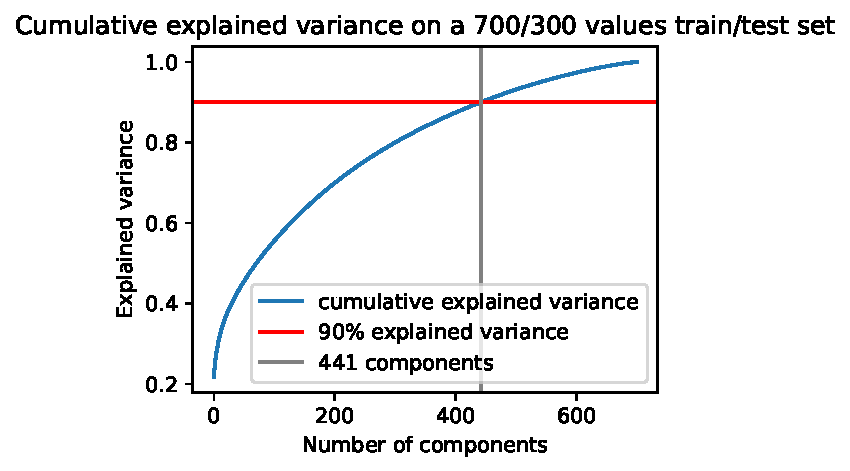
\includegraphics[width=7cm]{images/Eigendocs/Eval-Params/cumulative_explained_variance.pdf}}}%
    \qquad
    \subfloat[\centering The reconstruction error \ac{rmse} calculated for different values of $m$. Around 13 is an "elbow" point.]
    {{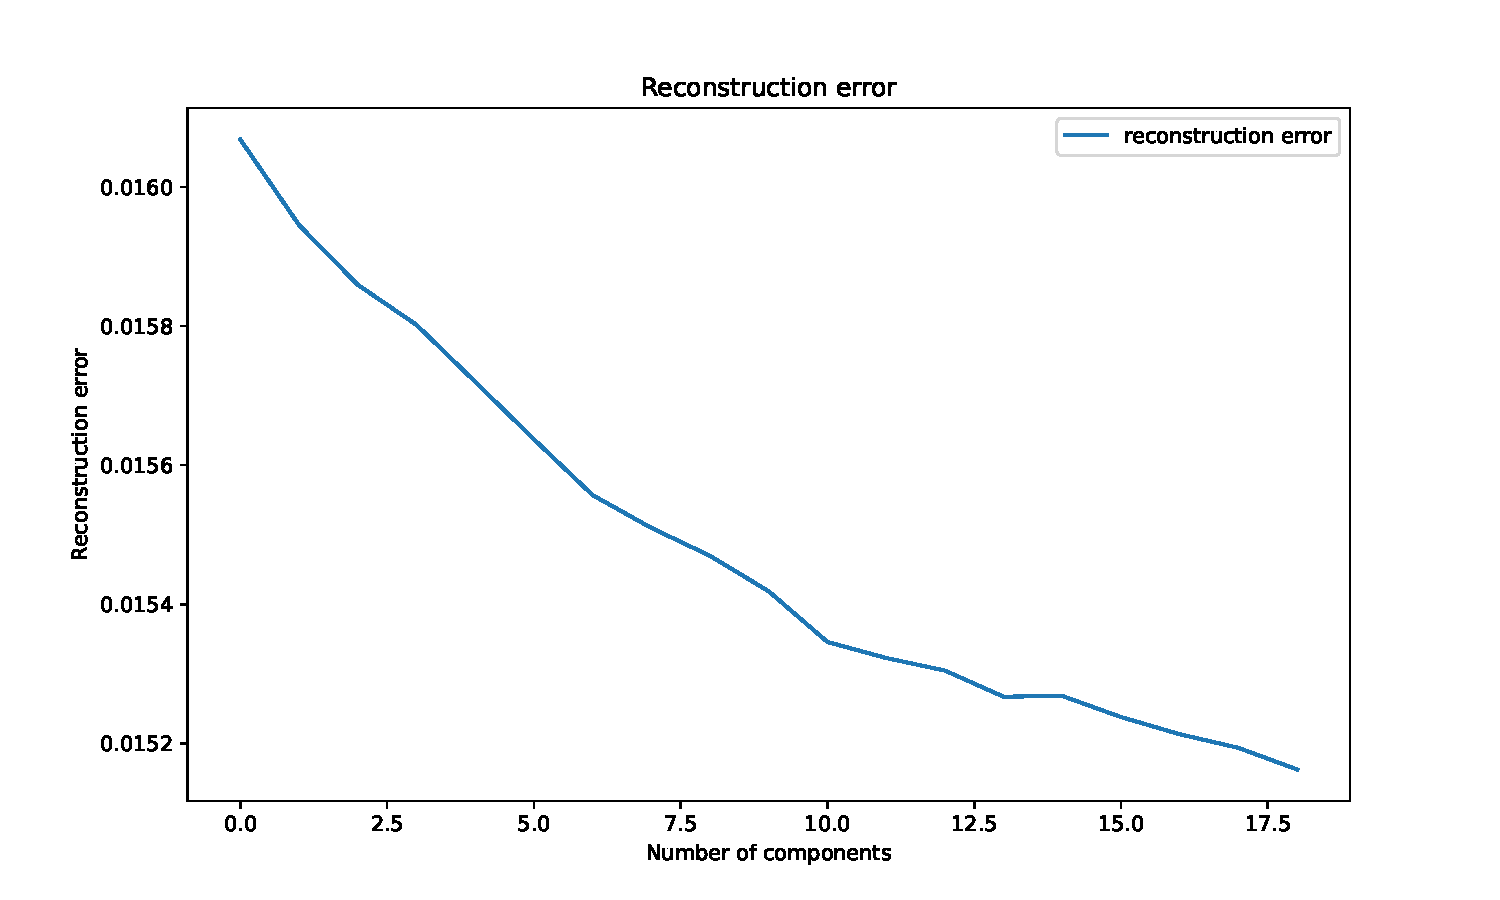
\includegraphics[width=7cm]{images/Eigendocs/Eval-Params/reconstruction error_eigendocs.pdf} }}%
    \caption[Approaches to find the number of \eigenfaces{}]{Two approaches in the literature to determine the number of \eigenfaces{} $m$ used to compress the input images.}%
    \label{fig:det_n_comp}%
\end{figure}

% calculation of eigenvectors of covariance matrix C
In order to reduce calculation complexity, $C$ is approximated.
% 1997
\citeauthor{eigenfaces1997} propose the approximation $\textbf{C} \simeq \frac{1}{N}\sum_{k=1}^{N}\textbf{x}_{k}\textbf{x}_{k}^{T} = \frac{1}{N}\textbf{X}\textbf{X}^{T}$, 
with $\textbf{X} = \left[ \textbf{x}_{1}, \textbf{x}_{2}, ..., \textbf{x}_{N} \right]$, $\textbf{x}_i \in \mathbb{R}^{n}$ \cite{eigenfaces1997}.

Finding the eigenvectors of $\textbf{X}\textbf{X}^{T}$ is still computationally expensive, since $\textbf{X}\textbf{X}^{T}$ is a $n$ by $n$ matrix.
According to \citeauthor{eigenfaces1997}, the eigenvectors of $\textbf{X}\textbf{X}^{T}$ can be calculated by using the eigenvectors of $\textbf{X}^{T}\textbf{X}$.
The eigenvalues $\textbf{e}_i \in \mathbb{R}^{n}$ of $\textbf{X}\textbf{X}^{T}$ can be derived from the eigenvectors $\textbf{v}_i \in \mathbb{R}^{N}$ of $\textbf{X}^{T}\textbf{X}$ by 
$\textbf{e}_i = \frac{1}{\sqrt{\lambda_i}}\textbf{X}\textbf{v}_i$ as discussed in more detail in \cite{eigenfaces1997}.
Hence, the problem is reduced to a $N$ by $N$ matrix, which is computationally less expensive to solve, since $N \ll n$.
Eigenvectors can be calculated using \ac{svd} \cite{eigenfaces1997}.
\ac{svd} is a method, which decomposes a matrix into the so-called left singular vector, the diagonal matrix and the right singular vector \cite{dim_reduction2021}. 
\ac{svd} facilitates the calculation of eigenvectors.

% classification/ compare
In the literature, face images are classified by comparing their position in the face space with those of already known faces \cite{eigenfaces1991}.
% performance 
According to \cite{eigenfaces1991}, this approach performs well on datasets with little variation in pose, lighting and facial expression.
However, \Citeauthor{eigenfaces1997} state, that the performance deteriorates if the variations increase since the changes introduce a bias 
that makes the distance function used to make classifications a no longer reliable measure.


\section{Clustering}\label{sec:clustering}

Clustering is used in a variety of domains to group data into meaningful subclasses \cite{OPTICS2013, OPTICS2014, OPTICS_kMeans_2016}.
According to \citeauthor{OPTICS2013} and \citeauthor{clusteringDocs2020}, common domains include anomaly detection, noise filtering, document clustering and image segmentation. 
The objective is to find clusters, which have a low inter-class similarity and a high intra-class similarity \cite{OPTICS2013}.
The similarity is measured by a distance function, which is dependent on the data type. 
Common distance functions are the Euclidean distance, the Manhattan distance and the Minkowski distance \cite{OPTICS_kMeans_2016}.

There are multiple clustering techniques, which can be divided into four categories \cite{OPTICS2016}: 
\begin{itemize}
    \item \textbf{Hierarchical clustering}:
    Algorithms, that create spherical or convex-shaped clusters, possibly naturally occurring. 
    A terminal condition has to be defined beforehand.
    Examples include CLINK, SLINK \cite{OPTICS2014} and \ac{optics} \cite{OPTICS2013}.

    \item \textbf{Partitional based clustering}: 
    Algorithms, that partition the data into $k$ clusters, $k$ is given apriori.
    Clusters are shaped in a spherical manner, are similar in size and not necessarily naturally occurring.
    KMeans is a popular example of a partitional-based clustering algorithm.

    \item \textbf{Density based clustering}:
    Density is defined as the number of objects within a certain distance of each other \cite{OPTICS_kMeans_2016}.
    The resulting clusters can be of arbitrary shape and size.
    The algorithm usually chooses the optimal number of clusters given the input data.
    However, some algorithms are sensitive to input parameters, such as radius, minimum number of points and threshold.
    Popular examples are \ac{dbscan} and \ac{optics}.
    
    \item \textbf{Grid based clustering}:
    Similar to density-based clustering, but according to \citeauthor{OPTICS2016} better than density-based clustering.
    Examples include flexible grid-based clustering \cite{OPTICS2014}.
    
\end{itemize}

Multiple approaches listed below use the term \textit{$\varepsilon$-neighbourhood}, which is defined as the set of all objects within a certain distance $\varepsilon$ of a given object \cite{OPTICS2013}.
In other words: $N_\varepsilon (x) = \left\{ y \in X | dist(x,y) \le \varepsilon, y \neq x \right\}$, $\varepsilon$ being the so-called generating distance.


%\subsection{KMeans}\label{subsec:kmeans}

KMeans partitions the data into $k \in \mathbb{N}$  clusters, $k$ is given apriori \cite{OPTICS_kMeans_2016,clusteringDocs2020}. %
First, $k$ centroids, i. e. cluster centres, are randomly initialized.
Then, the objects are assigned to the closest centroid.
Afterwards, the centroids are updated by calculating the mean of the assigned objects.
The process is repeated until the terminating condition, for instance, no more change in the clusters, is met \cite{OPTICS_kMeans_2016}.
By iteratively reassigning the objects to the closest centroid and updating the centroids, 
the algorithm minimizes the within-cluster sum of squared errors $E$, i. e. the sum of squared (Euclidean) distances between objects in a cluster and their centroid $\mu_{i}$, 
calculated in \autoref{eq:kmeans-error} from \cite{OPTICS_kMeans_2016}, 
where $C_{i}$ is the $i$-th cluster.

\begin{equation}
    E = \sum_{i=1}^{k} \sum_{x \in C_{i}}\left\|x-\mu_{i}\right\|^{2}
\label{eq:kmeans-error}
\end{equation}

\citeauthor{OPTICS_kMeans_2016} claim, that KMeans does not identify outliers.


\subsection{\acs*{dbscan}}\label{subsec:dbscan}

The clusters identified by \ac{dbscan} have a high density and are separated by low-density regions \cite{OPTICS_kMeans_2016}.
In order to create clusters of minimum size and density, \ac{dbscan} distinguishes between three types of objects \cite{OPTICS_kMeans_2016}:

\begin{itemize}
    \item \textbf{Core objects}: 
    An object $x$ with at least $minPts \in \mathbb{N}$ objects in its $\varepsilon$-neighbourhood $N_\varepsilon(x)$, i.e.\ $| N_\varepsilon (x) | \geq minPts$ is true \cite{OPTICS2013}.

    \item \textbf{Border objects}: 
    An object with less than $minPts$ objects in its $\varepsilon$-neighbourhood, which is in the $\varepsilon$-neighbourhood of a core object.

    \item \textbf{Noise objects}: 
    An object, which is neither a core object nor a border object.
\end{itemize}

\citeauthor{OPTICS_kMeans_2016} define $y \in X$ as \textit{directly density reachable} from $x \in X$, if $y$ is in the $\varepsilon$-neighbourhood of core object $x$ \cite{OPTICS_kMeans_2016}.
Moreover, a point $y \in X$ is \textit{density reachable} from $x \in X$, if there is a chain of objects $x_1, ..., x_n$ with $x_1 = x$ and $x_n = y$, 
which are directly density reachable from each other as displayed in \autoref{fig:density_reachable} \cite{OPTICS_kMeans_2016}.

\begin{figure}[!htb] % htp = hier (h), top (t), oder auf einer eigenen Seite (p).
    \centering
    \includesvg[width=0.2\textwidth]{images/density_reachable}
    \caption[Density reachability]{Density reachability cf. \cite{OPTICS1999}.
    The object $y \in X$ is density reachable from $x \in X$, since it exists a chain of directly density reachable objects between $x$ and $y$.
    }
    \label{fig:density_reachable}
\end{figure}

The objects $x \in X$ and $y \in X$ are said to be \textit{density connected}, if there is an object $o$, from which both $x$ and $y$ are density reachable \cite{OPTICS_kMeans_2016}.
Density connectivity is visualized in \autoref{fig:density_connected}.

\begin{figure}[!htb] % htp = hier (h), top (t), oder auf einer eigenen Seite (p).
    \centering
    \includesvg[width=0.2\textwidth]{images/density_connected}
    \caption[Density connectivity]{Density connectivity cf. \cite{OPTICS1999}.
    The objects $x$ and $y$ are density connected since there is an object $o$, from which both $x$ and $y$ are density reachable.
    }
    \label{fig:density_connected}
\end{figure}

The \ac{dbscan} algorithm starts by labeling all objects as core, border or noise points.
Then, it eliminates noise points and links all core points, which are within each other's neighbourhood \cite{OPTICS_kMeans_2016}.
Groups of connected core points form a cluster.
In the end, every border point is assigned to a cluster.
The non-core point cluster assigning is non-deterministic \cite{OPTICS2013}.
This algorithm creates clusters as a maximal set of density-connected points \cite{OPTICS_kMeans_2016}.

According to \citeauthor{OPTICS_kMeans_2016}, \ac{dbscan} can identify outliers or noise.
However, the algorithm is sensitive to the input parameters $minPts$ and $\varepsilon$ and has difficulties distinguishing closely located clusters \cite{OPTICS_kMeans_2016}.
Moreover, if one wants to obtain hierarchical clustering, one has to run the algorithm multiple times with different $\varepsilon$, which is expensive in terms of memory usage \cite{OPTICS2013}.
According to \citeauthor{clusteringDocs2020}, \ac{dbscan} is affected by the curse of dimensionality.
Since \ac{dbscan} relies on nearest neighbour queries and these become less meaningful in high dimensions, i.e.\ distances become difficult to interpret, 
the quality and accuracy of the results decline with increasing dimensionality \cite{clusteringDocs2020}.
\citeauthor{clusteringDocs2020} found that their \ac{dbscan} model assigns most objects noise when the dimensionality is sufficiently large.


\subsection{\acs*{optics}}\label{subsec:optics}

\ac{optics} does not return an explicit clustering, but rather a density-based clustering structure of the data, 
which is equivalent to repetitive clustering for a broad range of parameters \cite{OPTICS1999}.
\citeauthor{OPTICS1999} claim that real-world datasets cannot be described by a single global density, since they often consist of different local densities, 
as displayed in \autoref{fig:diff_density_cluster}.

\begin{figure}[!htb] % htp = hier (h), top (t), oder auf einer eigenen Seite (p).
    \centering
    \includesvg[width=0.4\textwidth]{images/diff_density_cluster}
    \caption[Clusters with different densities]{Clusters with different densities cf. \cite{OPTICS1999}.
    Since $C_1$ and $C_2$ have different densities than $A$ and $B$, a clustering algorithm using one global density parameter would detect the clusters $A$, $B$ and $C$, 
    rather than $A$, $B$, $C_1$ and $C_2$ .
    }
    \label{fig:diff_density_cluster}
\end{figure}

Opposed to \ac{dbscan}, \ac{optics} is able to detect clusters of varying densities \cite{OPTICS2014}.
\ac{optics} produces an order of the elements according to the distance to the already added elements \cite{OPTICS2014, OPTICS2013}:
The first element added to the order list is arbitrary.
%$\varepsilon$ defines the neighbourhood radius, i.e.\ the maximum distance between two elements, which are still considered to be in the same neighbourhood \cite{OPTICS_kMeans_2016}.
The order list is iteratively expanded by adding the element of the $\varepsilon$-neighbourhood to the order list, which has the smallest distance to any of the elements already in the order list.
Hence, clusters with higher density, i.e.\ lower $\varepsilon$, are added first (prioritized) \cite{OPTICS_kMeans_2016, OPTICS1999}.
When there are no more elements in the $\varepsilon$-neighbourhood to add, the process is repeated for the other clusters.
The non-core point cluster assigning is non-deterministic \cite{OPTICS2013}.

\begin{equation}
    RD(y) = \left\{
    \begin{array}{ll}
    \textrm{NULL} & \, \textrm{if |}N_\varepsilon (x)| < minPts \\
    max(core\_dist(x), dist(x,y)) & \, \textrm{otherwise} \\
    \end{array}
    \right. 
    \label{eq:optics-reachability-distance}
\end{equation}

\ac{optics} saves the reachability distance $RD(y)$, as calculated in \autoref{eq:optics-reachability-distance} from \cite{OPTICS2013},
with core distance $core\_dist$ being the minimal distance $\varepsilon^{min}$ such that $| N_{\varepsilon^{min}} (x) | \geq minPts$ 
(i.e.\ the distance to the $minPts^{th}$ point in $N_\varepsilon$) or NULL else, 
of each element $y$ to its predecessor $x$ in the order list and thus, 
a representation of the density necessary to keep two consecutive objects $x$ and $y$ in the same cluster \cite{OPTICS2013}.
If $\varepsilon < RD(y)$, then $y$ is not density reachable from any of its predecessors and thus, 
one can determine whether two points are in the same cluster for the information saved by \ac{optics} \cite{OPTICS2013, OPTICS1999}.
If the core distance of an element is not NULL, i.e.\ it is a core object, and it is not density reachable from its predecessors, it is the start of a new cluster \cite{OPTICS1999}.
Otherwise, the element is a noise point \cite{OPTICS1999}.
According to \citeauthor{OPTICS2013}, the algorithm builds a spanning tree, which enables obtaining the clusters for a given $\varepsilon$ by returning the connected components 
of the spanning tree after omitting all edges with $\varepsilon < RD(y)$ \cite{OPTICS2013}.
The relationship between $\varepsilon$, cluster density and nested density-based clusters is displayed in \autoref{fig:nested_density_cluster}.

% nested clusters, eps, fixed minPts
\begin{figure}[!htb] % htp = hier (h), top (t), oder auf einer eigenen Seite (p).
    \centering
    \includesvg[width=0.5\textwidth]{images/nested_density_cluster.svg}
    \caption[Relationship between $\varepsilon$, cluster density and nested density-based clusters]
    {The relationship between $\varepsilon$, cluster density and nested density-based clusters cf. \cite{OPTICS1999}.
    For a constant $minPts$, clusters with higher density such as $C_1$, $C_2$ and $C_3$, i.e.\ a low $\varepsilon_2$ value, 
    are completely contained in lower density clusters such as $C$ given $\varepsilon_1 > \varepsilon_2$.
    This idea forms the basis of \ac{optics} of expanding clusters iteratively and thus, 
    enables the detection of clusters for a broad range of neighbourhood radii $0 \le \varepsilon_i \le \varepsilon$.
    }
    \label{fig:nested_density_cluster}
\end{figure}

This procedure enables the extraction of clusters for arbitrary $0 \le \varepsilon_i \le \varepsilon$ \cite{OPTICS_kMeans_2016, OPTICS1999}.
According to \citeauthor{OPTICS2013}'s work, even though the clustering algorithm is expensive, the extraction only needs linear time.
According to \cite{OPTICS1999}, the algorithm yields good results if the input parameters $minPts$ and $\varepsilon$ are "large enough" and thus, the algorithm is rather insensitive to the input parameters.

% effect of eps (reachability plot)
The smaller $\varepsilon$ is chosen, the more objects will be identified as noise and thus, the algorithm will not identify clusters with low density, 
since some objects only become core objects for a larger $\varepsilon$ \cite{OPTICS1999}.
According to \citeauthor{OPTICS1999}, the optimal value for $\varepsilon$ creates one cluster for most of the objects with respect to a constant $minPts$,
since information about all density-based clusters for $\varepsilon_i < \varepsilon$ is preserved.
\citeauthor{OPTICS1999} present a heuristic for choosing $\varepsilon$ based on the expected $k$-nearest neighbour distance \cite{OPTICS1999}.

% effect of minPts (reachability plot)
High values for $minPts$ smoothen the reachability curve, even though the overall shape stays roughly the same \cite{OPTICS1999}.
According to \citeauthor{OPTICS1999}, the optimal value for $minPts$ is between 10 and 20.



\section{Database Elasticsearch}\label{sec:db}

% introduction, users
\databaseName{} is a widely used non-relational database, which was designed to store and perform full-text search on a large corpus of unstructured data \cite{Elasticsearch2017}.
This open-source distributed document-driven database system is built in Java and is based on the Apache Lucene (Java) library for high-speed full-text search \cite{Elasticsearch2017, Elasticsearch2019}.
According to \citeauthor{Elasticsearch2019}, \databaseName{} provides Wikipedia's full-text search and suggestions as well as Github's code search and Stack Overflow's geolocation queries and related questions.
It enables near real-time search by index refreshing periods of one second.
Needless to say, \databaseName{} is qualified to handle Big Data.

% structure
\databaseName{} is a document store, which stores schemaless key-value pairs called documents \cite{flask2018}.
The documents are stored in logical units, so-called indices.
% index
As stated by \citeauthor{Elasticsearch2019} and \citeauthor{Elasticsearch2017}, the indices are structured similarly to Apache Lucene's inverted index format.
An index can be spread into multiple nodes.
A node is a single running instance of \databaseName{} \cite{Elasticsearch2019}.
An index is divided into one or more shards, which can be stored on different servers and enable parallelization.
% Replicas
Replicas are copies of shards, which create redundancy and thus, ensure availability. %\cite{Elasticsearch2019}.

% document
The documents are saved in a \ac{json} format \cite{Elasticsearch2017}.
A document's fields and field types are defined by the user when initializing the database index.
By default, every field of a document is indexed and searchable \cite{Elasticsearch2019}.

% query (endpoints)
% get: search id
By specifying the unique \texttt{\_id} of a document and the database \texttt{index}, it is possible to retrieve a specific document from the database using the \texttt{GET \ac{api}}.
The query is real-time by default.
The parameters \texttt{\_source\_excludes} or \texttt{\_source\_includes} can be used to define the structure of the response \cite{Elasticsearch-get}.

% full-text search
The keyword used when performing a full-text search is \texttt{match}.
To query for a specific value, one has to specify the \texttt{<field>} of interest and the query value.

\databaseName{} preprocesses the query value before starting the search \cite{Elasticsearch-text-analyser}.
The default preprocessing steps of the so-called default analyzer include tokenization and lowercasing \cite{Elasticsearch-text-analyser}. 
Omitting stop words is disabled by default, but it is possible to provide custom stop words or use the English stop word list \cite{Elasticsearch-text-analyser}.
It is possible to create custom tokenizers, which split the query value into tokens of a certain maximum length.

Another useful feature of \databaseName{} is the multi-term synonym expansion.
When the user queries a specific phrase \databaseName{} expands the query to include synonyms of the query terms \cite{Elasticsearch-synonyms}.
The maximum number of expansion terms is set to 50 by default but can be configured by the user \cite{Elasticsearch-match}.
By default, the multi-terms synonym expansion option is enabled.

\databaseName{} also provides the option to perform fuzzy matching instead of exact search.
By enabling the fuzzy matching option, a \databaseName{} query consisting of for instance, \textit{Bahama} returns documents that contain the word \textit{Bahamas}.
By default, this option is not enabled but can be enabled and configured individually by the user \cite{Elasticsearch-match}.


% knn-search
Another search option of \databaseName{} is the \ac{knn} search.
The return value of a \ac{knn} search is the \texttt{k} nearest neighbours in terms of a certain distance function of a query vector \cite{Elasticsearch-kNN-HNSW}.
The query is a dense vector of the same dimension as the vectors stored in the database.
A \ac{knn} search either returns the exact brute-force nearest neighbours or 
an approximation of the nearest neighbours calculated by the \ac{hnsw} algorithm \cite{Elasticsearch-kNN-HNSW, Elasticsearch-knn}.
\ac{hnsw} is a graph-based algorithm \cite{Elasticsearch-kNN-HNSW}.
The term \texttt{navigable} refers to the graphs used, which are graphs with (poly-)logarithmic scaling of links traversed during greedy traversal concerning the network size \cite{Elasticsearch-kNN-HNSW}.
The idea of a \texttt{hiercharical} algorithm is to create a multilayer graph, grouping links according to their link length, as displayed in \autoref{fig:hnsw-layer}. 
The search starts on the uppermost layer, i.e. the layer containing the longest links, greedily traversing the layer until reaching the local minimum.
It uses this local minimum as the starting point at the next lower layer and the process is repeated until the lowest layer is reached \cite{Elasticsearch-kNN-HNSW}.
The layers of the graph are built incrementally, and a neighbour selection heuristic, as depicted in \autoref{fig:hnsw-heuristic}, not only creates links between close elements, 
but also between isolated clusters to ensure global connectivity \cite{Elasticsearch-kNN-HNSW}.

\begin{figure}[htp] % htp = hier (h), top (t), oder auf einer eigenen Seite (p).
    \centering
    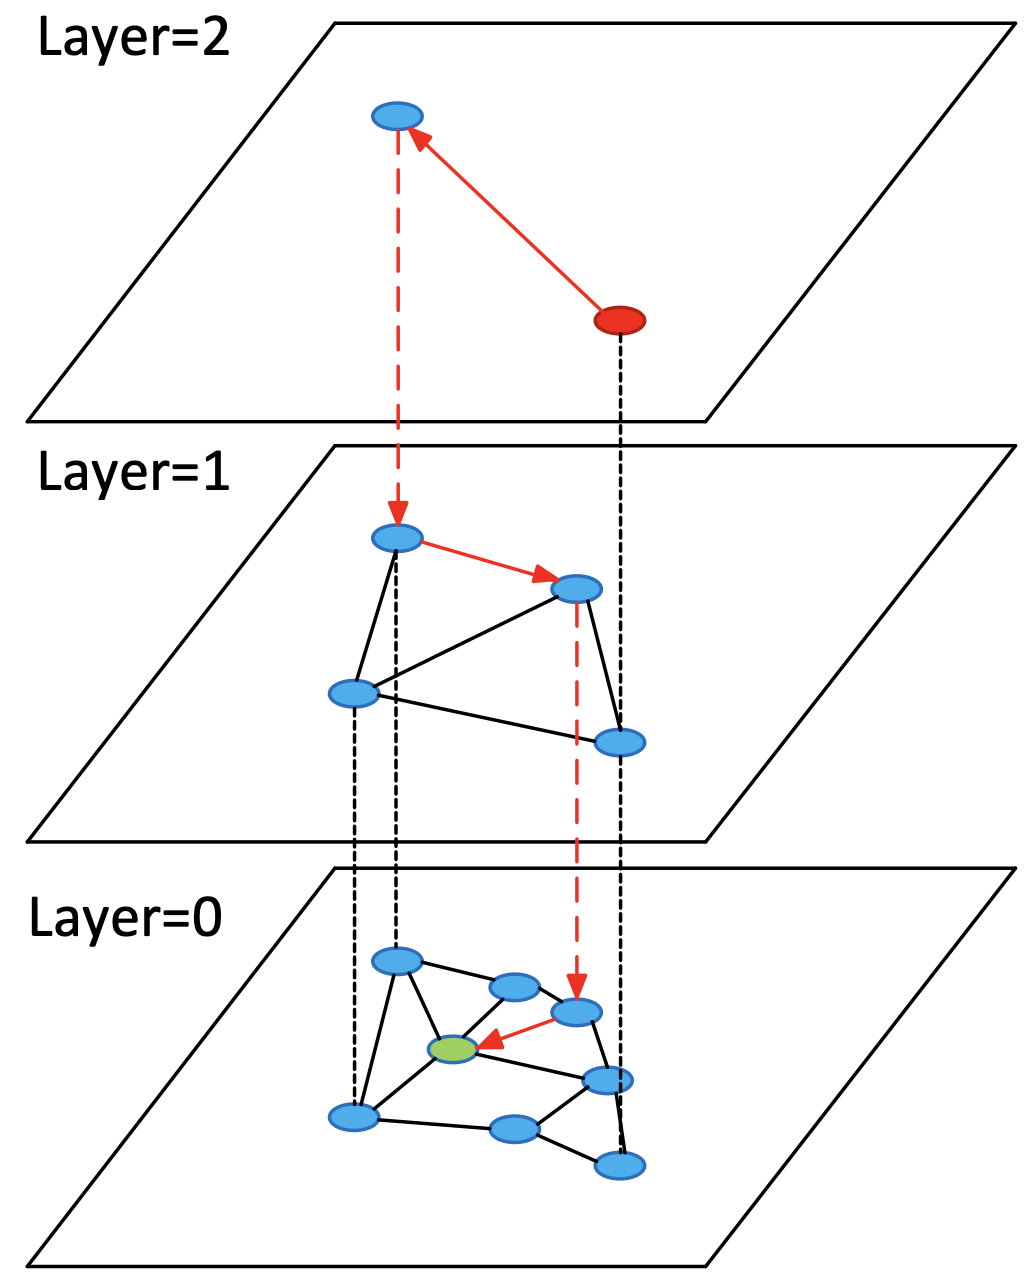
\includegraphics[width=0.3\textwidth]{images/Elasticsearch/HNSW-layer.png}
    \caption[Structure of \ac{hnsw} layers]{Structure of \ac{hnsw} layers from \cite{Elasticsearch-kNN-HNSW}.
    The search starts on the uppermost layer, i.e. the layer containing the longest links, greedily traversing the layer until reaching the local minimum.
    The local minimum is used as the starting point at the next lower layer and the process is repeated until the lowest layer is reached.
    }
    \label{fig:hnsw-layer}
\end{figure}

\begin{figure}[htp] % htp = hier (h), top (t), oder auf einer eigenen Seite (p).
    \centering
    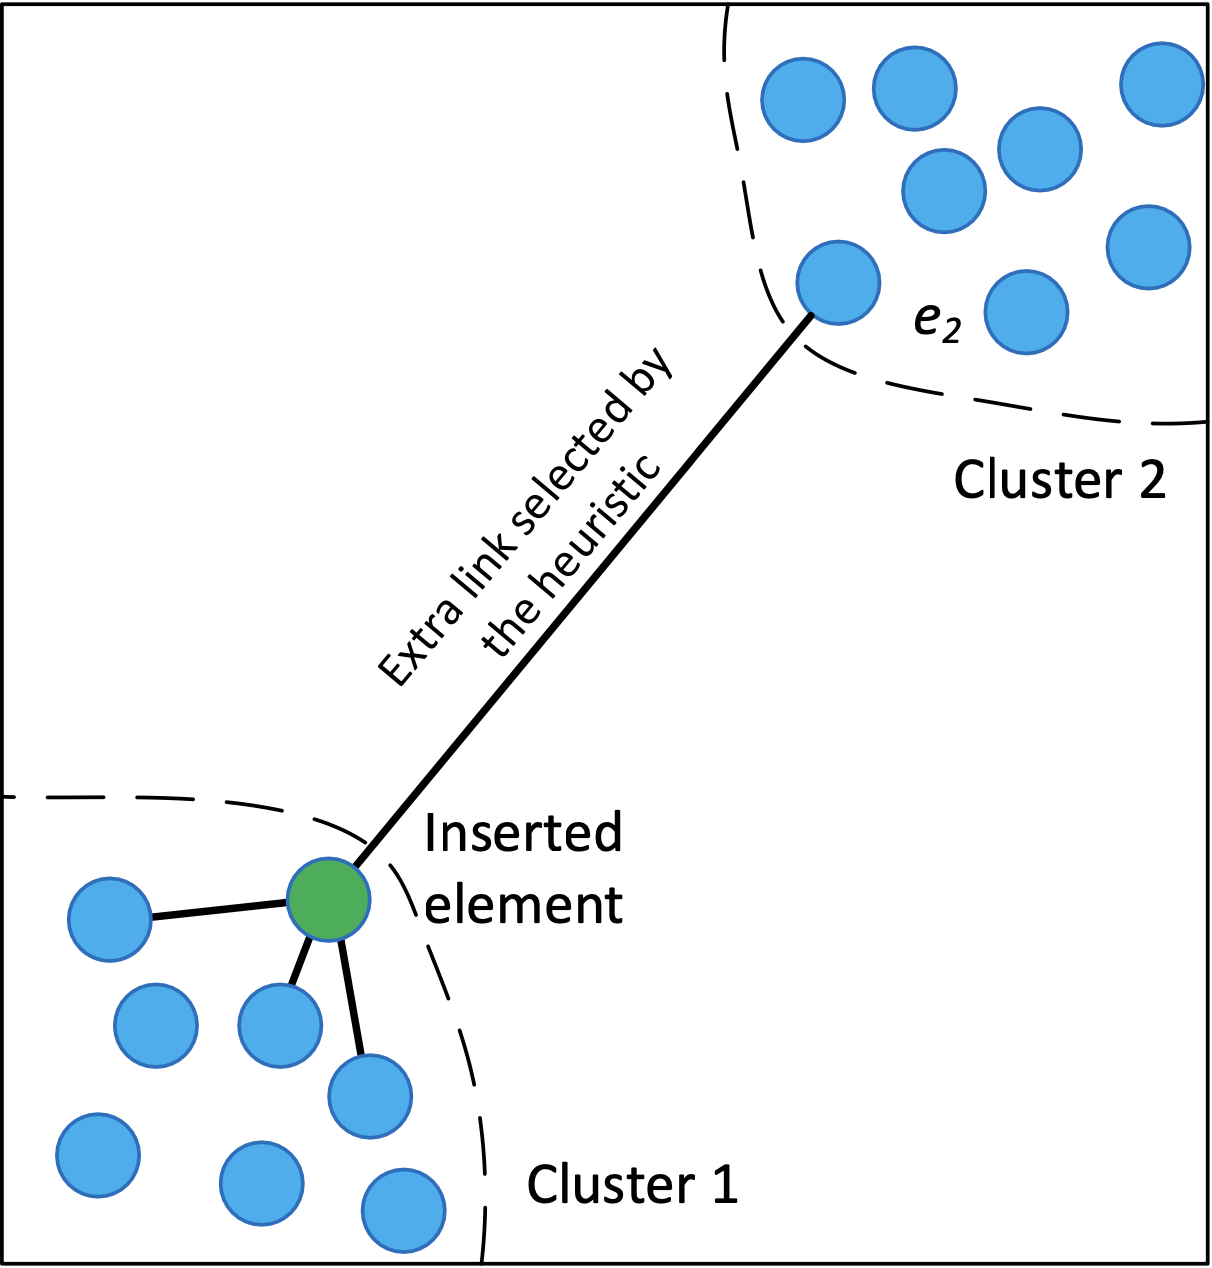
\includegraphics[width=0.3\textwidth]{images/Elasticsearch/HNSW-neighbour-selection-heuristic.png}
    \caption[Neighbour selection heuristic of \ac{hnsw}]{Neighbour selection heuristic of \ac{hnsw} from \cite{Elasticsearch-kNN-HNSW}.
    The heuristic creates diverse links, i.e. links between close elements (e.g., green circle and elements in cluster 1) 
    and between isolated clusters (e.g., green circle and $e_2$) to ensure global connectivity.
    }
    \label{fig:hnsw-heuristic}
\end{figure}

In order to perform \ac{knn} search on a \texttt{<field>} it has to be of type \texttt{dense\_vector}, indexed and a \texttt{similarity} measure has to be defined when initializing the database \cite{Elasticsearch-knn}.
\databaseName{}'s \ac{knn} implementation not only allows literal matching on search terms but also semantic search \cite{Elasticsearch-knn}.

Besides \databaseName{}, the elastic stack offers other tools, for instance, Kibana, which provides a user interface to manage different models.
After saving a model in Kibana, it is possible to create a text embedding ingest pipeline, which embeds new documents or reindexes existing documents \cite{Elasticsearch-knn-embedding}.



\section{\flask{}}\label{sec:BE_flask}

% introduction
\flask{} is open source and written in Python by Armin Ronancher in 2004 \cite{flask2015, mvc_flask2019}.
According to \citeauthor{flask_book2015} and \citeauthor{mvc_flask2019}, \flask{} is one of the most popular Python web frameworks.
It provides powerful libraries for core functionality such as routing, templating, and \ac{http} request parsing \cite{flask_book2015}.
It is extensible and thus, can be extended with additional plugins without affecting the internal structure of the existing system \cite{flask2015}.

% technical details
\flask{} uses the Jinja Template Engine for template files including \ac{html} pages,
whereas static files such as \ac{css} files are handeled using the Werkzeug WSGI toolkit \cite{flask2015}.
According to \citeauthor{flask2015}, Jinja is modeled after the Django template system.
Werkzeug implements, for instance, requests and response objects \cite{mvc_flask2019}.

% initialization
All requests received from clients are passed to an instance of the \flask{} application \cite{flask_book2018}.
Hence, the first step is to create an instance of the \flask{} class, such as done in \lst{lst:flask_app_init}.

\begin{listing}[htp]
    \begin{minted}{python3}
    app = Flask(__name__)
    \end{minted}
    \caption[Initialization of \flask{} application instance]{Initialization of \flask{} application instance.
    }
    \label{lst:flask_app_init}
\end{listing}

% routing
Clients send requests to the web server, which passes them to the \flask{} application instance.
The queries are then routed to the corresponding functions.
Routing is the process of mapping \ac{url} paths to functions \cite{flask_book2018}.
To define a route, the \texttt{route} decorator is used as displayed in \lst{lst:flask_routing}.

\begin{listing}[htp]
    \begin{minted}{python3}
    @api.route('/documents/<id>', endpoint='document')
    class Document(Resource):
        def get(self, id):
            elastic_search_client = Elasticsearch(CLIENT_ADDR)
            return query_database.get_doc_meta_data(elastic_search_client, 
                doc_id=id)
    \end{minted}
    \caption[Routing using \flask{}]{Exemplartary definition of a function to display routing with \flask{}.
    The \texttt{route} decorator is used to define the \ac{url} path.
    }
    \label{lst:flask_routing}
\end{listing}

\acs{url} can contain dynamic components, which are enclosed in \texttt{<>} angle brackets.
The values of these components are passed to the function as arguments \cite{flask_book2018}.
By default, dynamic components are of type \texttt{string}.
However, other types including \texttt{int} and \texttt{float} are supported \cite{flask_book2018}.

% dev server
During development, the \flask{} application can be run using \texttt{flask run} to start the built-in development web server \cite{flask_book2018}.
By enabling debug mode, the server automatically reloads the application when changes are detected \cite{flask_book2018}.

% endpoints
An endpoint is a class with certain methods, which can be accessed using \ac{http} requests.
Every endpoint can have multiple decorators, including \texttt{GET}, \texttt{POST}, \texttt{PUT} and \texttt{DELETE} \cite{flask2018}.
The \texttt{GET} method is used to retrieve data from the server, whereas the other methods are used to either insert, update or delete data.


\section{\angular{}}\label{sec:FE_angular}

\angular{} is a framework for building web applications.
It uses Node.js and TypeScript.
Usually, the source code is structured into different modules, including components and services.
Components are used to define the appearance of the application, while
service modules contain the logic of the application and communicate with the backend.

% creating applications
\angular{} applications are created using the \texttt{ng new NAME} command line interface \cite{angular_book2018}.
This command creates a skeleton, which can be customized to meet the needs of the application.
By running \texttt{ng serve} the application can be served locally.
    \chapter{Implementation}\label{ch:implementation}

This chapter describes how the theoretical basics from \autoref{ch:methodology} interplay and how they are used in this thesis.
In this thesis, a tool is developed that offers text queries, detailed document inspection and queries for semantically or visually similar documents to the user.
\autoref{sec:offline-processing} outlines the steps carried out before the application is operative, 
\autoref{sec:ui} is about the resulting application and 
\autoref{sec:trade-off} discusses the dilemma faced when balancing memory usage and query time. 
Specific parameter choices are explained in \autoref{ch:evaluation}.


\section{Offline Processing}\label{sec:offline-processing}
This section outlines implementation details of the data fed into the database, the database itself and the baseline topic analysis approach compared to this work's application.
 % Database
\subsection{Database}\label{subsec:impl-db}
First, the content of the \databaseName{} database is described, then, the initialization, insertion and updating process of filling the database are explained 
and finally, the process of querying is outlined.

% content
\subsubsection*{Content of the database}
In this work, the database is filled once with data from a large unstructured corpus of \ac{pdf} files.
After the initialization of the database, it is used for queries. 
Therefore, the workflow is completely offline.

The index \textit{Bahamas} stores different embeddings of the information derived from the text layer and metadata of the documents.
As depicted in \autoref{fig:pdf2db}, not only textual information is stored in the database, 
but also information about the appearance of the first page of the \ac{pdf}.
The structure of the index is presented in \autoref{tbl:Elasticsearch-fields}.

\begin{table}[]
    \caption{Fields of the \databaseName{} database index \textit{Bahamas}.}
    \begin{tabular}{|
    >{\columncolor[HTML]{EFEFEF}}l |p{0.63\textwidth}|}
    \hline
    \cellcolor[HTML]{C0C0C0}\textbf{Field name} & \cellcolor[HTML]{C0C0C0}\textbf{Field description}                                     \\ \hline
    \_id                                        & Unique identifier of document \texttt{i}. The identifier is generated by the sha256 hash algorithm from hashlib using the \ac{pdf} file as input.\\ \hline
    doc2vec                                     & 55 dimensional \ac{d2v} embedding of \texttt{i}.                                                          \\ \hline
    sim\_docs\_tfidf                            & \ac{tfidf} embedding + all-zero flag of \texttt{i}. The all-zero flag is one if the \ac{tfidf} embedding consists of only zeros, zero else. If the embedding's dimensionality is greater than 2048, the encoder of a trained \ac{ae} is used to compress the embedding.\\ \hline
    google\_univ\_sent\_encoding                & 512 dimensional \ac{use} embedding of \texttt{i}.                                     \\ \hline
    huggingface\_sent\_transformer              & 384 dimensional \ac{sbert} embedding of \texttt{i}.                                  \\ \hline
    inferSent\_AE                               & \infersent{} embedding of \texttt{i}. Since the pretrained \infersent{} model embedding's dimension is 4096, the encoder of a trained \ac{ae} has to reduce the dimension to 2048.                                                    \\ \hline
    pca\_image                                  & 13-dimensional \ac{pca} version of first page image of \texttt{i}.                      \\ \hline
    pca\_optics\_cluster                        & Cluster of \texttt{i} identified by \acs{optics} on \ac{pca} version of image.            \\ \hline
    argmax\_pca\_cluster                        & Number of maximum \ac{pca} component as cluster of \texttt{i}.                            \\ \hline
    text                                        & Text of \texttt{i}.                                                                       \\ \hline
    path                                        & Path to \texttt{i}.                                                     \\ \hline
    \end{tabular}
    \label{tbl:Elasticsearch-fields}
\end{table}

\begin{figure}[!htb] % htp = hier (h), top (t), oder auf einer eigenen Seite (p).
    \centering
    \includesvg[width=1\textwidth]{images/Elasticsearch/PDFs_to_database}
    \caption[Database procedure]{\acp{pdf} to Database. 
    First, the data is preprocessed:
    The first page of a \ac{pdf} file is converted to an image and the complete text is extracted. 
    The images are stored in the database as well as the text and different embeddings of the text.
    Some values, such as the image or the \infersent{} embedding, have to be compressed to become a vector of at most 2048 dimensions.
    }
    \label{fig:pdf2db}
\end{figure}

% initialize, insert, update
\subsubsection*{Initialization, insertion and updating}
To facilitate working with and running the code the initialization of the database is split into multiple steps.
As depicted in \autoref{fig:init_db}, first the database is initialized by defining the index name and the mappings, i. e. the field names, types and sizes.
This step is carried out using the method \texttt{create}.

\begin{figure}[!htb] % htp = hier (h), top (t), oder auf einer eigenen Seite (p).
    \centering
    \includesvg[width=0.5\textwidth]{images/Elasticsearch/init_db.svg}
    \caption[Initialization and filling of the database]{Procedure of initialization and filling of the database.}
    \label{fig:init_db}
\end{figure}

Afterwards, the documents are created using the method \texttt{create}.
The initial creation of a document only defines the fields \texttt{id}, \texttt{text} and \texttt{path}.
% In order to maximise efficiency when updating the database, the \databaseName{}'s built-in functionality \texttt{bulk} is used.
% \texttt{bulk} sends chunks of multiple requests to the database.
% As displayed in \lst{lst:db_bulk}, \texttt{bulk} is called with the \databaseName{} client, 
% a function which yields requests and parameters, which define the return values.
% The structure of a function that yields requests is shown in \lst{lst:db_bulk_yield}.

% \begin{listing}[htp]
%     \begin{minted}{python3}
%         bulk(client, create_document_aux(src_paths, client), stats_only= True)
%     \end{minted}
%     \caption[Usage of \databaseName{}'s helper functionality \texttt{bulk}]
%     {Usage of \databaseName{}'s helper functionality \texttt{bulk} to send multiple requests to the database in chunks.
%     }
%     \label{lst:db_bulk}
% \end{listing}

% \begin{listing}[htp]
%     \begin{minted}{python3}
%         def create_document_aux(src_paths: list, client: Elasticsearch):  
%             for path in src_paths:           
%                 id = get_hash_file(path)
%                 if get_doc_meta_data(client, doc_id=id) is not None:
%                     continue
%                 text = pdf_to_str(path)
%                 yield { '_op_type': 'create',
%                         '_index': 'bahamas',
%                         '_id': id,
%                         "text": text,
%                         "path": path}
%     \end{minted}
%     \caption[Method that yields requests for \texttt{bulk}]
%     {Method that yields requests for \texttt{bulk}.
%     The method checks if the document is already in the database and if not, it yields a request to create the document.
%     }
%     \label{lst:db_bulk_yield}
% \end{listing}

The embeddings are added to the documents in a third step.
% To make sure that it is possible to update embeddings individually without changing other fields, 
% a method to insert the embeddings of a specific model for all documents is created.
% The documents are updated using the \texttt{update} keyword and \texttt{bulk}.
To increase the efficiency of this step, data parallelism, i. e. parallelizing the execution of a method across multiple input values, is applied.
In this work, the data to be split among multiple processes is a set of paths to documents.
The \texttt{Pool} object from the multiprocessing module is used for data parallelism.
The steps carried out are displayed in \lst{lst:db_Pool_embeddings}.
First, the absolute paths of all documents are saved in a list.
This list is divided in \texttt{num\_cpus} many sublists of similar size.
Each process works on a sublist.
The embeddings are subsequentially inserted into the database for each sublist. 

\begin{listing}[htp]
    \begin{minted}{python3}
        with Pool(processes=num_cpus) as pool:
            for model_name in model_names:
                proc_wrap = wrapper(model_name=model_name, baseDir=src_path)
                pool.map(proc_wrap, sub_lists)
    \end{minted}
    \caption[Usage of \texttt{Pool} for data parallelism]
    {Usage of \texttt{Pool} for data parallelism.
    The paths to the documents to insert are divided into sublists which are simultaneously inserted into the database.
    Since the \texttt{Pool} object does not work with a \texttt{lambda} function, 
    a class \texttt{wrapper} is created which provides the same functionality.
    }
    \label{lst:db_Pool_embeddings}
\end{listing}

The document embeddings are added to the database using the method \texttt{update} as displayed in \lst{lst:db_Pool_update}.

\begin{listing}[htp]
    \begin{minted}{python3}
        client.update(index='bahamas', id=id, body={'doc': 
            {MODELS2EMB[model_name]: embedding}})
    \end{minted}
    \caption[Update of a database entry]
    {Update of a database entry to insert a specific embedding.
    }
    \label{lst:db_Pool_update}
\end{listing}


% search
\subsubsection*{Queries}
The default analyzer is used for the full-text search since for instance configuring a maximum token length did not seem necessary or likely to improve the results.

\begin{listing}[htp]
    \begin{minted}{python3}
        results = elastic_search_client.search(
            index='bahamas', 
            size=count,
            from_=(page*count),
            query= {'match': {
                        'text': {'query':text,
                                'fuzziness': 'AUTO',}
                    }, 
                }, source_includes=SRC_INCLUDES)
    \end{minted}
    \caption[Query to an \databaseName{} database index]{Exemplary query to an \databaseName{} database index.
    The parameters \texttt{size} and \texttt{from\_} define the number of results to return and the start index of the results.
    To enable fuzzy search a value for \texttt{fuzziness} has to be set. 
    }
    \label{lst:fuzzy_query}
\end{listing}

Moreover, the fuzzy matching option is set to \texttt{AUTO}, which means in terms of keyword or text fields that the allowed Levenshtein Edit Distance, 
i. e. number of characters changed to create an exact match between two terms, to be considered a match, is correlated to the length of the term \cite{Elasticsearch-fuzziness}.
By default, terms of length up to two characters must match exactly, terms of length three to five characters must have an edit distance of one and 
terms of length six or more characters must have an edit distance of two \cite{Elasticsearch-fuzziness}.
An exemplary query, which uses fuzzy search is given in \lst{lst:fuzzy_query}.

According to \citeauthor{Elasticsearch-kNN-HNSW}, one of \ac{knn} search's use cases is semantic document retrieval, which makes it a good fit for this task.
In this work, the approximate nearest neighbours search is used, since it is faster and the results are good enough for the purpose of this work.
The similarity measure used in this work is the cosine similarity, which calculates the \texttt{\_score} of a document according to \autoref{eq:cosine-similarity-db} from \cite{Elasticsearch-kNN-similarity}, 
where \texttt{query} is the query vector and \texttt{vector} is the vector representation of the document in the database.
The other similarity measures provided by \databaseName{} are \texttt{l2\_norm} or 
so-called Euclidian distance and \texttt{dot\_product} which is the non-auto-normalized version of the \texttt{cosine} option.
Since cosine is not defined on vectors with zero magnitude, embeddings that can return all zero vector representations, such as \ac{tfidf}, 
are enhanced with an all-zero flag before inserting them into the database.

\begin{equation}
    \frac{1 + \text{cosine}(\text{query}, \text{vector})}{2}
    \label{eq:cosine-similarity-db}
\end{equation}

In this work, the only tool from the elastic stack used is \databaseName{}.
Without Kibana, the used models are saved on disk as \ac{pkl} files.
Consequently, instead of using the \ac{knn} query structure for semantic search on embeddings provided by \databaseName{}, the normal \ac{knn} search on a field that contains an embedding is used.

% Eigendocs
\section{\eigendocs{}}\label{subsec:eigendocs}

% this work
\begin{figure}[htp] % htp = hier (h), top (t), oder auf einer eigenen Seite (p).
    \centering
    \includesvg[width=1.0\textwidth]{images/eigendocs}
    \caption[\eigendocs{} procedure]{From \acp{pdf} to \eigendocs{}.
    Firstly, the first page of a document is converted to an image.
    Then, the image is preprocessed:
    It is placed on a white canvas, to ensure all images have the same dimensions.
    Moreover, it is converted to greyscale and normalized to values between zero and one.
    Afterwards, the 2d image is reshaped to a 1d array.
    Lastly, the image is compressed using \eigendocs{}.
    }
    \label{fig:eigendocs_procedure}
\end{figure}

In this work, the \eigenfaces{} approach from \autoref{subsec:eigenface} is used to compress the images of the first page of documents.
The idea is that documents not only hold textual information but also visual information, such as layout, company logo or signature.
By mapping those images on a subspace, they ought to be grouped by visual similarity.
The procedure of the \eigenfaces{} adaption \textit{\eigendocs{}} is displayed in \autoref{fig:eigendocs_procedure}.

% procedure
The documents are first read from a directory. 
Subsequently, their first page is converted to an image and saved.
When initially filling the database, these images are read from their directory.
Firstly, the maximum height and width among all images in the corpus is calculated.
These dimensions are used to create a white canvas for each image which forms the background.
Every image is placed in the upper left corner.
Hence, assuming the selection of documents used to fit the \ac{pca} model is representative, 
scaling is not necessary and thus, the portion of white pixels on the right and bottom side encodes the dimension of the former image.
However, some images are bigger than the max values from selected data and as a consequence are scaled.
Therefore, the relative size of images in the corpus is incorporated in the resulting representation of the input images.

\begin{listing}[htp]
    \begin{minted}{python3}
        C = np.ones((max_w,max_h))
        C[:doc.shape[0],:doc.shape[1]] = rgb2gray(doc)
        documents.append(C.ravel())
    \end{minted}
    \caption{Preprocessing of the input images from \thesissupervisor{}.
    The background is a white canvas.
    The images are converted to one-dimensional greyscale values.}
    \label{lst:preproc_images}
\end{listing}

Afterwards, they are converted to greyscale images using \lst{lst:rgb2grey}.
Before returning the image, the two-dimensional image vectors are converted to one-dimensional ones as displayed in the last line of \lst{lst:preproc_images}.
The decomposition is transformed using \ac{pca} as displayed in \lst{lst:pca_svd}.
The implementation of \ac{pca} from \href{https://scikit-learn.org/stable/modules/generated/sklearn.decomposition.PCA.html}{sklearn} 
intrinsically normalizes the data as described in \autoref{subsec:eigenface} and thus, does not require the user to manually preprocess the data.


\begin{listing}[htp]
    \begin{minted}{python3}
        0.299*img[:,:,0] + 0.587*img[:,:,1] + 0.114*img[:,:,2]
    \end{minted}
    \caption{Conversion of RGB pixel values to greyscale from a script by \thesissupervisor{}.}
    \label{lst:rgb2grey}
\end{listing}

\begin{listing}[htp]
    \begin{minted}{python3}
        pca = decomposition.PCA(n_components=n_components, whiten=True, 
            svd_solver="randomized")
    \end{minted}
    \caption{Initialization of the \ac{pca} instace used to compress the image data.
    Since the \eigenfaces{} approach uses a svd\_solver, the adaption \eigendocs{} has to be implemented likewise.
    }
    \label{lst:pca_svd}
\end{listing}




% Embeddings
\subsection{Embeddings}\label{subsec:impl-embeddings}
The models used to encode the textual data from the data corpus are outlined below with regard to implementation details.

\subsubsection*{\ac{tfidf}}\label{subsubsec:impl-tfidf}

% overall architecture
The \ac{tfidf} model has to be initialized and trained on the data corpus to build a data-specific vocabulary.
An exemplary implementation is given in \lst{lst:impl-tfidf}.
The \texttt{TfidfVectorizer} is provided by the \texttt{scikit-learn} package.
When initializing the model, the parameters define not only the input type but also the way the data is preprocessed.
The \texttt{input} parameter defines the input type, i.e.\ \texttt{content} means that the input is a list of strings or bytes, 
whereas \texttt{file} assumes the input has a \texttt{read} method and \texttt{filename} denotes a list of filenames as input \cite{tfidf-scikit-learn}.
An embedding is obtained using the command from \lst{lst:encode-tfidf}.

\begin{listing}[htp]
    \begin{minted}{python3}
        tfidf_model = TfidfVectorizer(input='content', 
                    preprocessor=TfidfTextPreprocessor().transform, min_df=3, 
                    max_df=int(len(docs)*0.07))
        tfidf_model.fit(documents)
    \end{minted}
    \caption[Initialization of the \ac{tfidf} model]{Initialization of the \ac{tfidf} model.
    Firstly, an instance of the \texttt{TfidfVectorizer} class is created.
    Secondly, the \texttt{fit} method is called to fit the model on the documents.
    }
    \label{lst:impl-tfidf}
\end{listing}

\begin{listing}[htp]
    \begin{minted}{python3}
        tfidf_model.transform(text).todense()
    \end{minted}
    \caption[Encoding a text using the \ac{tfidf} model]{Encoding a text using the \ac{tfidf} model.
    }
    \label{lst:encode-tfidf}
\end{listing}

The \texttt{preprocessor} parameter defines the preprocessing, i.e.\ string transformation, stage.
It is possible to override the default with a custom preprocessing function.
The parameters \texttt{min\_df} and \texttt{max\_df} define the minimum and maximum document frequency of a word in the corpus to be considered relevant.
The default values are $1$, i.e.\ a term has to appear at least once, and $1.0$, i.e.\ a term appears at most in all documents, respectively \cite{tfidf-scikit-learn}.

By default, the \texttt{scikit-learn} implementation uses the \texttt{norm='l2'} parameter, i.e.\ the Euclidean norm \cite{tfidf-scikit-learn}.
The implementation of \ac{tfidf} in \texttt{scikit-learn} is different from the original \ac{tfidf} definition.
The difference is the calculation of the \ac{idf} part, which is given in \autoref{eq:tfidf-scikit-learn} from \cite{tfidf-scikit-learn}.
The one is added to $M_{ij}$ due to the parameter \texttt{smooth\_id=True} by default to prevent zero divisions \cite{tfidf-scikit-learn}
and to avoid logarithmic divergences due to a zero argument \cite{glove2014}.
After calculating the \ac{tfidf} values, they are normalized by the Euclidean norm 
$v_{norm} = \frac{v}{\left\| v \right\|_{2}} = \frac{v}{\sqrt{v_1^{2} + v_2^{2} + ... + v_M^{2}}}$.

\begin{equation}
    \text{idf}(w_{ij}) = \log \frac{1 + M}{1 + M_{ij}} + 1    
    \label{eq:tfidf-scikit-learn}
\end{equation}

% pipeline
In this work, the text of the PDFs is first extracted, then preprocessed using a custom preprocessor and afterwards embedded using the \texttt{TfidfVectorizer}.
The \ac{tfidf} weights are the embedding.
Before storing the \ac{tfidf} weights in the database, they are enhanced with an all-zero flag.
The all-zero flag ensures that no all-zero vectors are stored in the database by extending those that have a zero magnitude with a "1" entry and "0" otherwise.
All-zero \ac{tfidf} weights indicate that a document does not have any terms with the vocabulary in common.
Since the vocabulary is kept relatively small with respect to the number of different words in the data corpus to reduce the dimensionality of the embeddings, 
it is not unlikely that a document does not contain any of the vocabulary terms.
The all-zero flag is necessary because the cosine similarity used to query for similar documents in the database cannot handle vectors of zero magnitude.
This alteration does not change the cosine similarity between non-zero magnitude vectors, 
since the additional zero adds no supplementary information to the calculation of the cosine similarity.
The vectors with a one in the all-zero flag column have a cosine similarity of one.
The pipeline in \autoref{fig:tfidf_embedding} visualizes these steps.

\begin{figure}[!htb] % htp = hier (h), top (t), oder auf einer eigenen Seite (p).
    \centering
    \includesvg[width=1\textwidth]{images/embeddings/tfidf/TFIDF_embedding.svg}
    \caption[\acs*{tfidf} pipeline]{\acs*{tfidf} pipeline.
    Firstly, the text extracted from the documents is preprocessed using a custom preprocessor.
    Then, the \acs*{tfidf} values are obtained from the \texttt{TfidfVectorizer}.
    Afterwards, the all-zero flag is added to the \acs*{tfidf} weights.
    If the resulting dimensionality is bigger than 2048, the encoder of an \acs*{ae} is used to reduce the dimensionality.
    The results are stored in the database.
    }
    \label{fig:tfidf_embedding}
\end{figure}


\begin{figure}[!htb] % htp = hier (h), top (t), oder auf einer eigenen Seite (p).
    \centering
    \includesvg[width=1\textwidth]{images/embeddings/tfidf/TFIDF_preprocessing.svg}
    \caption[Preprocessing]{Preprocessing visualized using an example text.
    The stop word removal implicitly tokenizes the text.}
    \label{fig:preprocessing}
\end{figure}

% custom preprocessing
In this work, a custom preprocessing function is used.
The preprocessing steps are visualized in \autoref{fig:preprocessing}.
Firstly, the accents are stripped from the text.
Then, all new line symbols are replaced with a whitespace.
Afterwards, the text is converted to lowercase.
Then the numbers are discretized, i.e.\ all numbers between 0 and 99999 are replaced with the string \texttt{SMALLNUMBER}, 
numbers bigger than 99999 are replaced with the string \texttt{BIGNUMBER} and floats are replaced with the string \texttt{FLOAT}.
The next step is to remove all punctuation symbols.
To ensure empty tokens generated by prior preprocessing steps are omitted, 
all sequences of multiple subsequent whitespaces are discarded.
After that, the symbols for numbers are enclosed with pointed brackets, e.g. \texttt{<SMALLNUMBER>}.
Then, the text is tokenized, i.e.\ split at whitespaces, and stop words are omitted.
The stop word list is provided by the \texttt{nltk} package 
and consists of common English stop words.
Afterwards, the tokens are lemmatized.
The lemmatizer used is \texttt{WordNetLemmatizer} from the \texttt{nltk} package.
\texttt{WordNetLemmatizer} uses the English lexical database \texttt{WordNet} to return valid stems \cite{nltk-lemma-wordnet}
In the end, the tokens are joined to a string and returned.

% Autoencoder
Since the dimensionality of the \ac{tfidf} embeddings is big for a large text corpus, 
an \ac{ae} is used to reduce the dimensionality of the embedding if its dimensionality exceeds 2048.

\subsubsection*{\ac{d2v}}\label{subsubsec:impl-doc2vec}

The library \texttt{gensim} provides the \ac{d2v} model used in this work.
The model is initialized with input data of type \texttt{tagged documents}, which are documents with (numerical) tags.
In this work, the default parameters are used.
%The parameter \texttt{dm} determines the training algorithm used.
%The value \texttt{dm=1} specifies the \ac{pvdm} algorithm, while \texttt{dm=0} specifies the \ac{pvdbow} algorithm \cite{gensim-doc2vec}.
The default algorithm is \ac{pvdm} \cite{gensim-word2vec-init}.
The parameters \texttt{vector\_size} and \texttt{window} define the dimensionality of the embeddings and the size of the window, 
i.e.\ the maximum distance between the current and the predicted word, respectively.
The default value for \texttt{vector\_size} is 100, whereas the default window size is 8 \cite{gensim-word2vec-init, gensim-doc2vec-init}.
The \texttt{min\_count} parameter defines a threshold below which words will be ignored.
Its default value is 5.
The \texttt{workers} parameter denotes the number of threads to be used for training.
The default value is 1 \cite{gensim-word2vec-init}.
The \texttt{epochs} parameter specifies the number of iterations over the corpus.
The default value is 10.
By default, the hierarchical softmax algorithm, i.e.\ \texttt{hs=1}, is used for training \cite{gensim-doc2vec}.
Many \ac{d2v} default values are adopted from \ac{w2v} since the \texttt{gensim} \ac{d2v} implementation inherits from the \ac{w2v} implementation.


\subsubsection*{\infersent{}}\label{subsubsec:impl-infersent}

% parameters
The \infersent{} model is implemented using PyTorch \cite{HfsentTrans2019}.
The parameters used to initialize the model are presented in \lst{lst:infersent-params}.
The parameter \texttt{version} in line \ref{line:infersent_version} indicates whether 
the model is trained with \acs{glove} or fastText for the value 1 or 2 respectively.
Since the model is precomputed, it is not possible to change certain parameters, 
such as the word embedding dimension \texttt{word\_emb\_dim} or the dimension of the output vectors \texttt{enc\_lstm\_dim}.

\begin{listing}[htp]
    \begin{minted}[escapeinside=||]{python3}
        'bsize': 64, 
        'word_emb_dim': 300, 
        'enc_lstm_dim': 2048,  
        'pool_type': 'max', 
        'dpout_model': 0.0, 
        'version': 1|\phantomsection\label{line:infersent_version}|
    \end{minted}
    \caption{Parameters of the \infersent{} model.
    }
    \label{lst:infersent-params}
\end{listing}

% state dict
The steps necessary to create a working instance of the \infersent{} model are presented in \lst{lst:infersent-init}.
After the \infersent{} model is initialized in line \ref{line:init}, the \texttt{state\_dict} of the model is loaded in line \ref{line:state_dict}.
This dictionary consists of learnable parameters, i.e.\ weights and bias, of the model.
The \texttt{state\_dict} is obtained from the \ac{pkl} file of \infersent{} as stated in \cite{download-infersent}.
The path to the word embeddings is set in line \ref{line:w2v_path}.
Finally, in line \ref{line:vocab}, the vocabulary of the model is built. 
More precisely, only those embeddings needed are kept while the rest is discarded.

\begin{listing}[htp]
    \begin{minted}[escapeinside=||]{python3}
        infersent = InferSent(params_model)|\phantomsection\label{line:init}|
        infersent.load_state_dict(torch.load(model_path))|\phantomsection\label{line:state_dict}|
        infersent.set_w2v_path(w2v_path)|\phantomsection\label{line:w2v_path}|
        infersent.build_vocab(docs, tokenize=True)|\phantomsection\label{line:vocab}|
    \end{minted}
    \caption{Initializing the \infersent{} model.
    }
    \label{lst:infersent-init}
\end{listing}

% GloVe
% Initially, in this work, the \infersent{} model was based on \acs{glove} word embeddings.
% \acs{glove} is a global log-bilinear regression model for unsupervised learning of vector representations of words \cite{glove2014}. 
% According to \citeauthor{glove2014}, the model captures global corpus statistics directly.
% %The complexity of the model is bound by $O(V^2)$, $V$ being the vocabulary size.
% %However, \citeauthor{glove2014} claim it is better than the worst case stated above and rather in $O(C)$, $C$ being the corpus size.
% The \acs{glove} model is trained on ratios of co-occurrence probabilities of words from the corpus, 
% which correlate with the relationship between the words. % \cite{glove2014}.
% \citeauthor{glove2014} introduce rules for a weighting function to ensure neither rare nor frequent co-occurrences are overweighted.
% It is possible to download embeddings computed by \acs{glove}, instead of using the algorithm to generate them.
% The precomputed word embeddings are stored in a 5.65 \ac{gb} text file.
% The file contains 840 B tokens and a vocabulary of 2.2 M cased 300-dimensional vector representations of words \cite{download-glove}.
% According to \citeauthor{UniversalSentEnc2018}, \acs{glove} introduces bias in terms of ageism, racism and sexism into the model.

% own W2V
In this work, a custom set of vector representations of words is used.
The custom word embeddings are computed by a \ac{w2v} model trained on 2048 randomly selected documents from the Bahamas dataset 
which reduces the run time of the script.
The only parameter which differs from the default settings of \ac{w2v} is the \texttt{vector\_size} which is set to 300.
After the \ac{w2v} model is trained, the word embeddings are saved in a file 
whose file path is the value of \texttt{w2v\_path} in line \ref{line:w2v_path} of \lst{lst:infersent-params}.
% The file is post-processed to be compatible with the \infersent{} model.
% To be more precise, only lines that consist of at least two whitespace-separated char sequences are kept.
% Usually, word embeddings stored in a text file are structured in a way that 
% the first char sequence is the word and the following numbers are the vector representation of the word.

% Autoencoder
In this work, an \ac{ae} is used to reduce the dimensionality of the \infersent{} embedding.


\subsubsection*{\ac{use}}\label{subsubsec:impl-use}

The \ac{use} model implemented with TensorFlow \cite{HfsentTrans2019}.
In this work, the fourth version of the model is used.
The implementation from Tfhub uses the \ac{dan} architecture \cite{UniversalSentEnc-dev}.
The file is about 1 \ac{gb}. % and thus, loading the model takes a while.
It is not necessary to preprocess the data for the model \cite{UniversalSentEnc-dev}.

\section{\ac{sbert}}\label{sec:impl-sbert}

The \ac{sbert} model is provided by PyTorch \cite{HfsentTrans2019}.
An instance of the model is obtained by initializing it as shown in \lst{lst:impl-sbert}.
The model consists of a \ac{bert} transformer, which has a \texttt{max\_seq\_length} of $128$. 
It does not convert inputs to lowercase by default \cite{sbert-dev}.
The output of the transformer is passed to a pooling layer, which is initialized with the \texttt{pooling\_mode} parameter.
The default is \texttt{mean\_pooling}, which calculates the mean of the output vectors of the transformer.
The other options are \texttt{cls\_token\_pooling}, which returns the output of the first token, 
\texttt{max\_pooling}, which returns the maximum value of the output vectors,
and \texttt{pooling\_mode\_mean\_sqrt\_len\_tokens}.
The word embedding dimension is 384 by default \cite{sbert-dev}.

\begin{listing}[htp]
    \begin{minted}{python3}
        SentenceTransformer('paraphrase-MiniLM-L6-v2')
    \end{minted}
    \caption[Initialization of the \ac{sbert} model]{Initialization of the \ac{sbert} model.
    }
    \label{lst:impl-sbert}
\end{listing}

\subsubsection*{\acl{ae}}\label{subsubsec:impl-autoencoder}

In this work, an \ac{ae} is used to reduce the dimensionality of the \infersent{} and the \ac{tfidf} embeddings.
Since the \infersent{} model is pretrained, it is not possible to change the dimensionality of the embedding without a considerably big effort,
i.e.\ retraining the model on a sufficiently large data corpus and reconfiguring the model's parameters.
Therefore, it is not feasible to change the dimensionality of the \infersent{} embedding, but rather add a supplementary layer after the model 
to produce the final embedding.
Similarly, the \ac{tfidf} embedding dimension correlates with the vocabulary size and thus, the size of the data corpus.
Further reducing the vocabulary size would decrease the \ac{tfidf} model's quality.
Hence, the idea is to use the encoder of an \ac{ae} to reduce the dimensionality of the \infersent{} and the \ac{tfidf} embedding.

\begin{figure}[!htb] % htp = hier (h), top (t), oder auf einer eigenen Seite (p).
    \centering
    \includesvg[width=1.0\textwidth]{images/embeddings/autoencoder/autoencoder-impl.svg}
    \caption[Architecture of the \acs*{ae}]{Architecture of the \acs*{ae}.}
    \label{fig:impl-ae}
\end{figure}

The implementation was provided by the blog post from \cite{impl-src-ae}.
It uses the library keras\footnote{https://keras.io/ (last accessed: 19/11/2023)}.
The architecture is adapted to fulfil the needs of the specific context.
It is presented in \autoref{fig:impl-ae}.

% Clustering
\subsection{Clustering using \acs*{optics}}\label{subsec:impl-optics}

\begin{figure}[!htb] % htp = hier (h), top (t), oder auf einer eigenen Seite (p).
    \centering
    \includesvg[width=1\textwidth]{images/OPTICS/OPTICS_procedure.svg}
    \caption[\ac{optics} procedure]{The first page of each document is converted to an image.
    The image is preprocessed, i.e. conversion to greyscale and resizing.
    }
    \label{fig:OPTICS_procedure}
\end{figure}

Similar to the approach from \citeauthor{OPTICS1999}, \ac{optics} is used to cluster the images of the first page of documents in this work.
The procedure is displayed in \autoref{fig:OPTICS_procedure}.
There were two different preprocessing approaches:
\begin{enumerate}
    \item \label{pt:32}The images were first preprocessed to 32x32 normalized greyscale pixels (cf. \cite{OPTICS1999}) as visualized in \autoref{fig:preprocessed_docs_32x32}
    and afterwards compressed to 13-dimensional vectors using \ac{pca}.
    \item \label{pt:eigendocs}The technique \eigendocs{} from \autoref{subsec:eigenface} 
    was used to compress the images to 13-dimensional normalized greyscale images as displayed in \autoref{fig:preprocessed_docs_eigendocs}.
\end{enumerate}


% preprocessed images
\begin{figure}[!htb] % htp = hier (h), top (t), oder auf einer eigenen Seite (p).
    \centering
    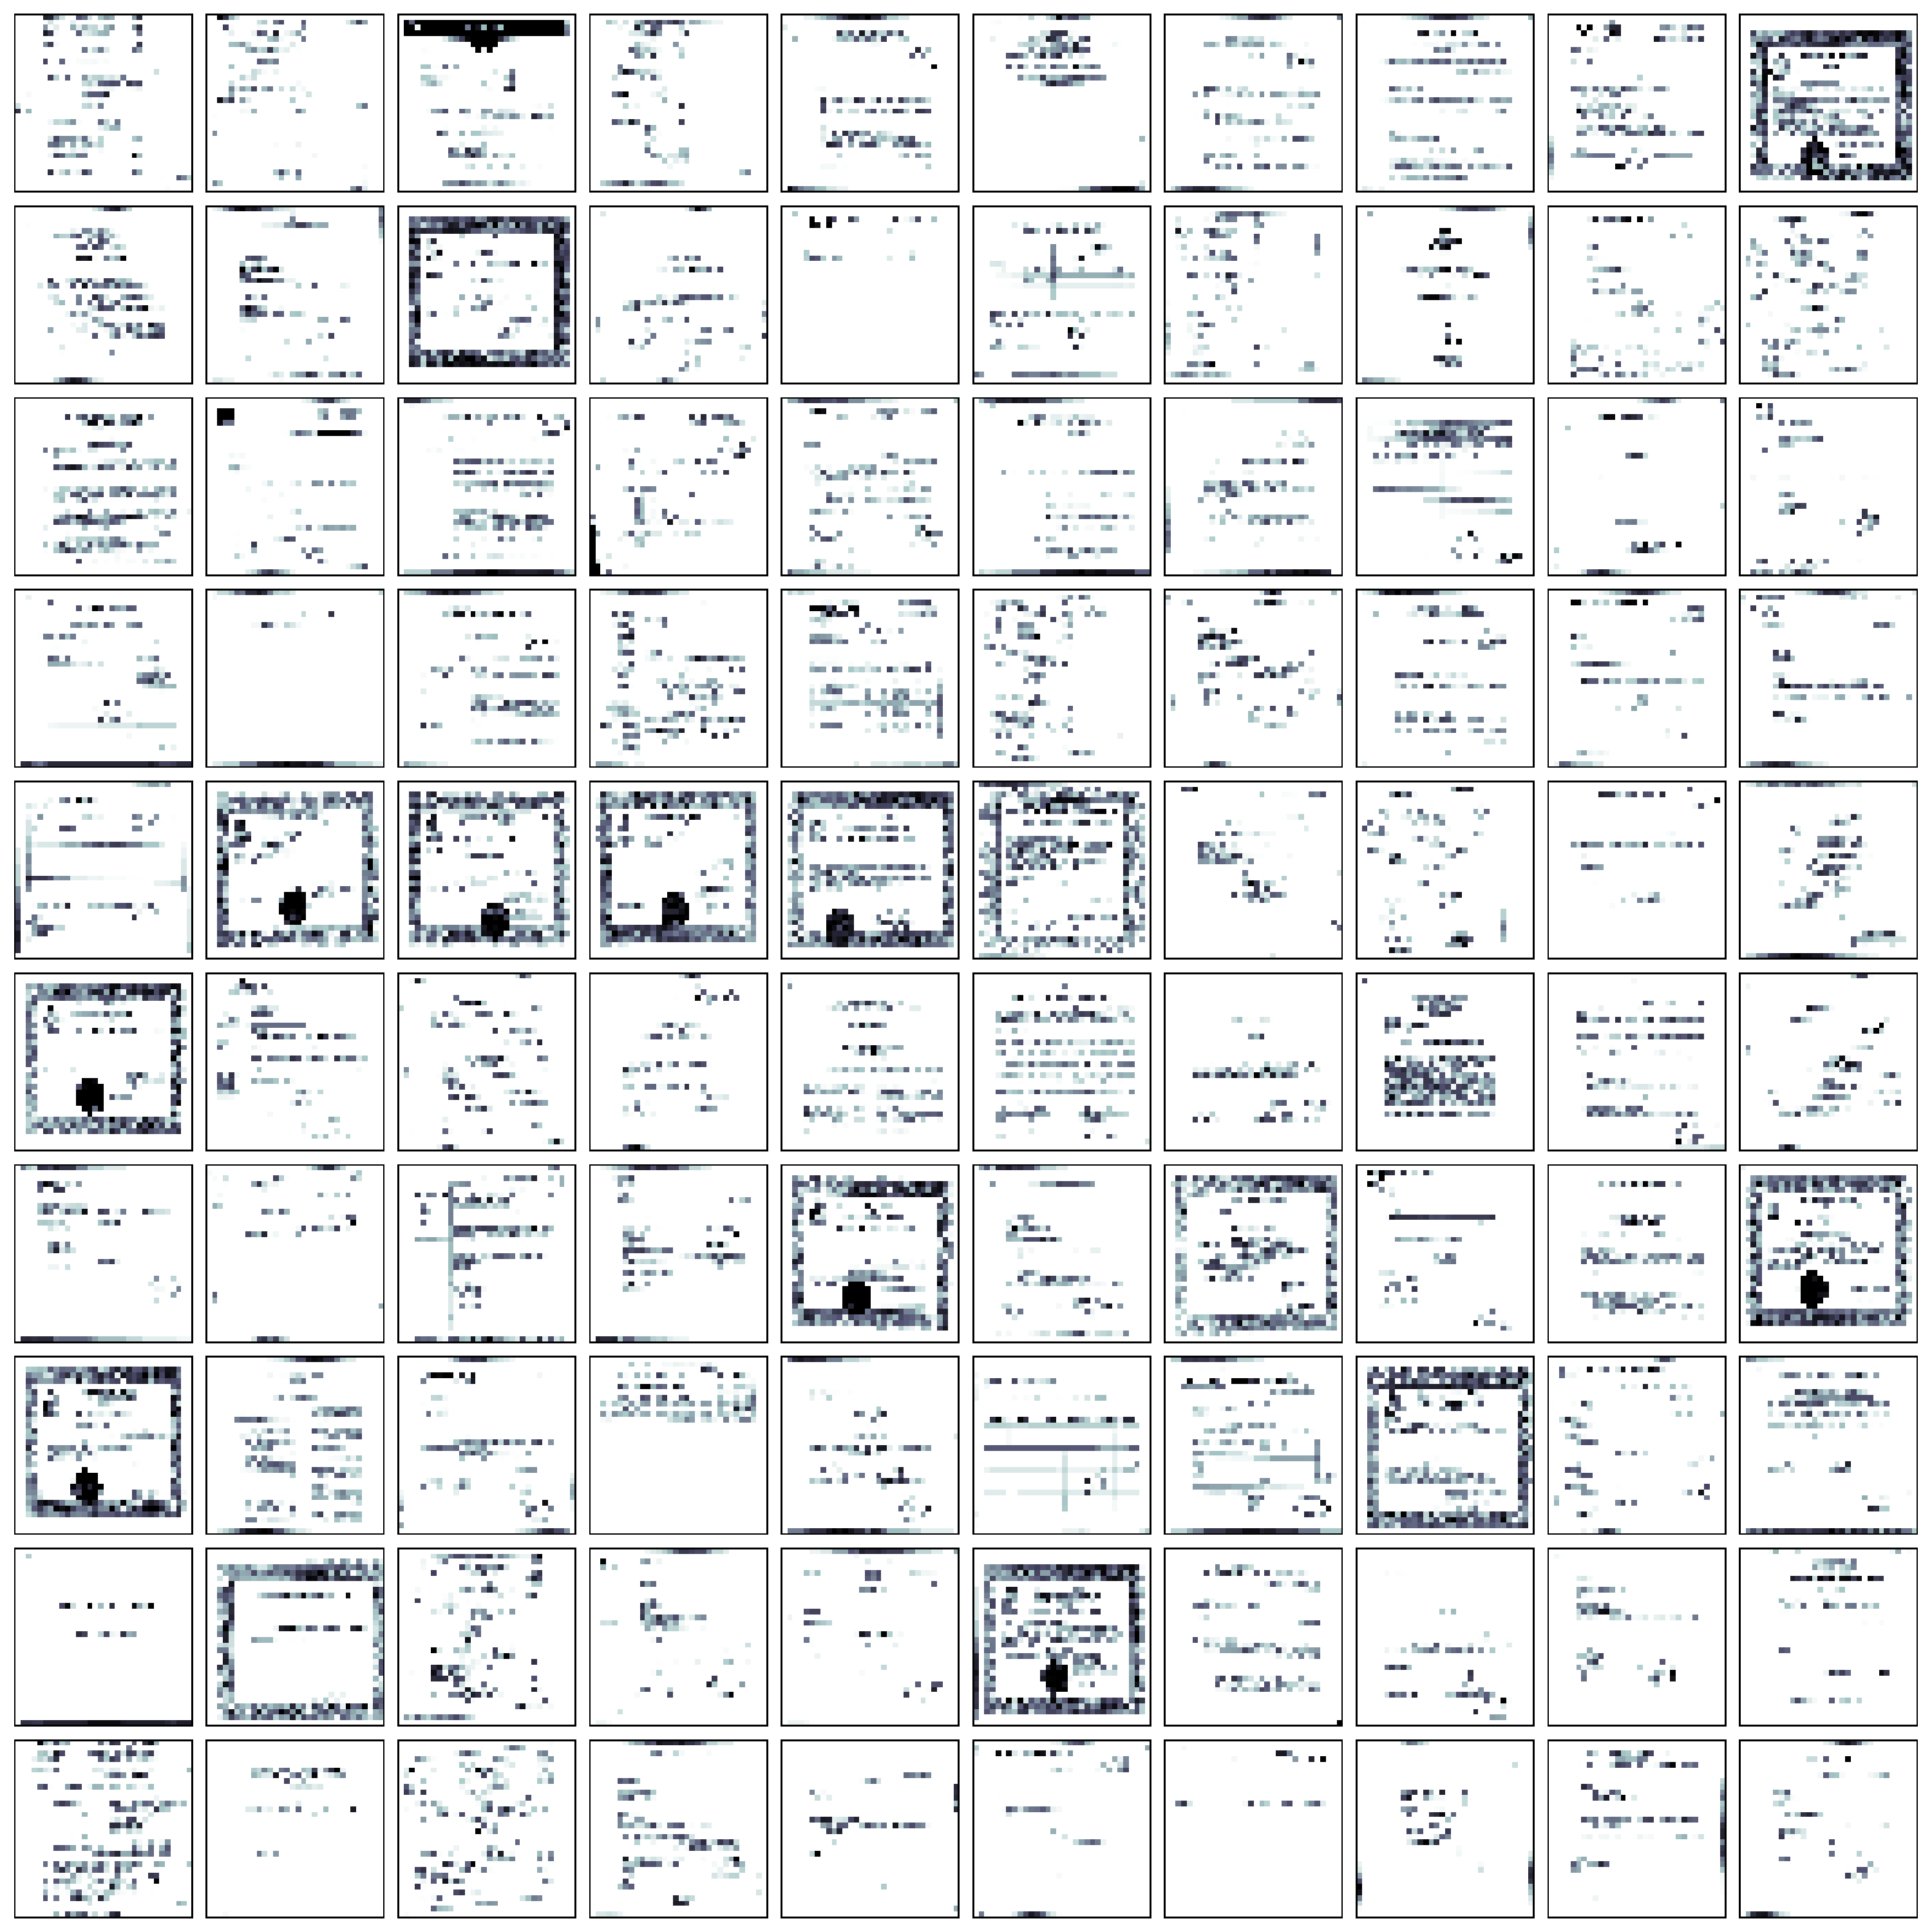
\includegraphics[width=1\textwidth]{images/OPTICS/32x32/preprocessed_docs.pdf}
    \caption[Preprocessing to 32x32 normalized greyscale pixels]{Preprocessing of 100 documents to 32x32 normalized greyscale pixels.
    }
    \label{fig:preprocessed_docs_32x32}
\end{figure}


\begin{figure}[!htb] % htp = hier (h), top (t), oder auf einer eigenen Seite (p).
    \centering
    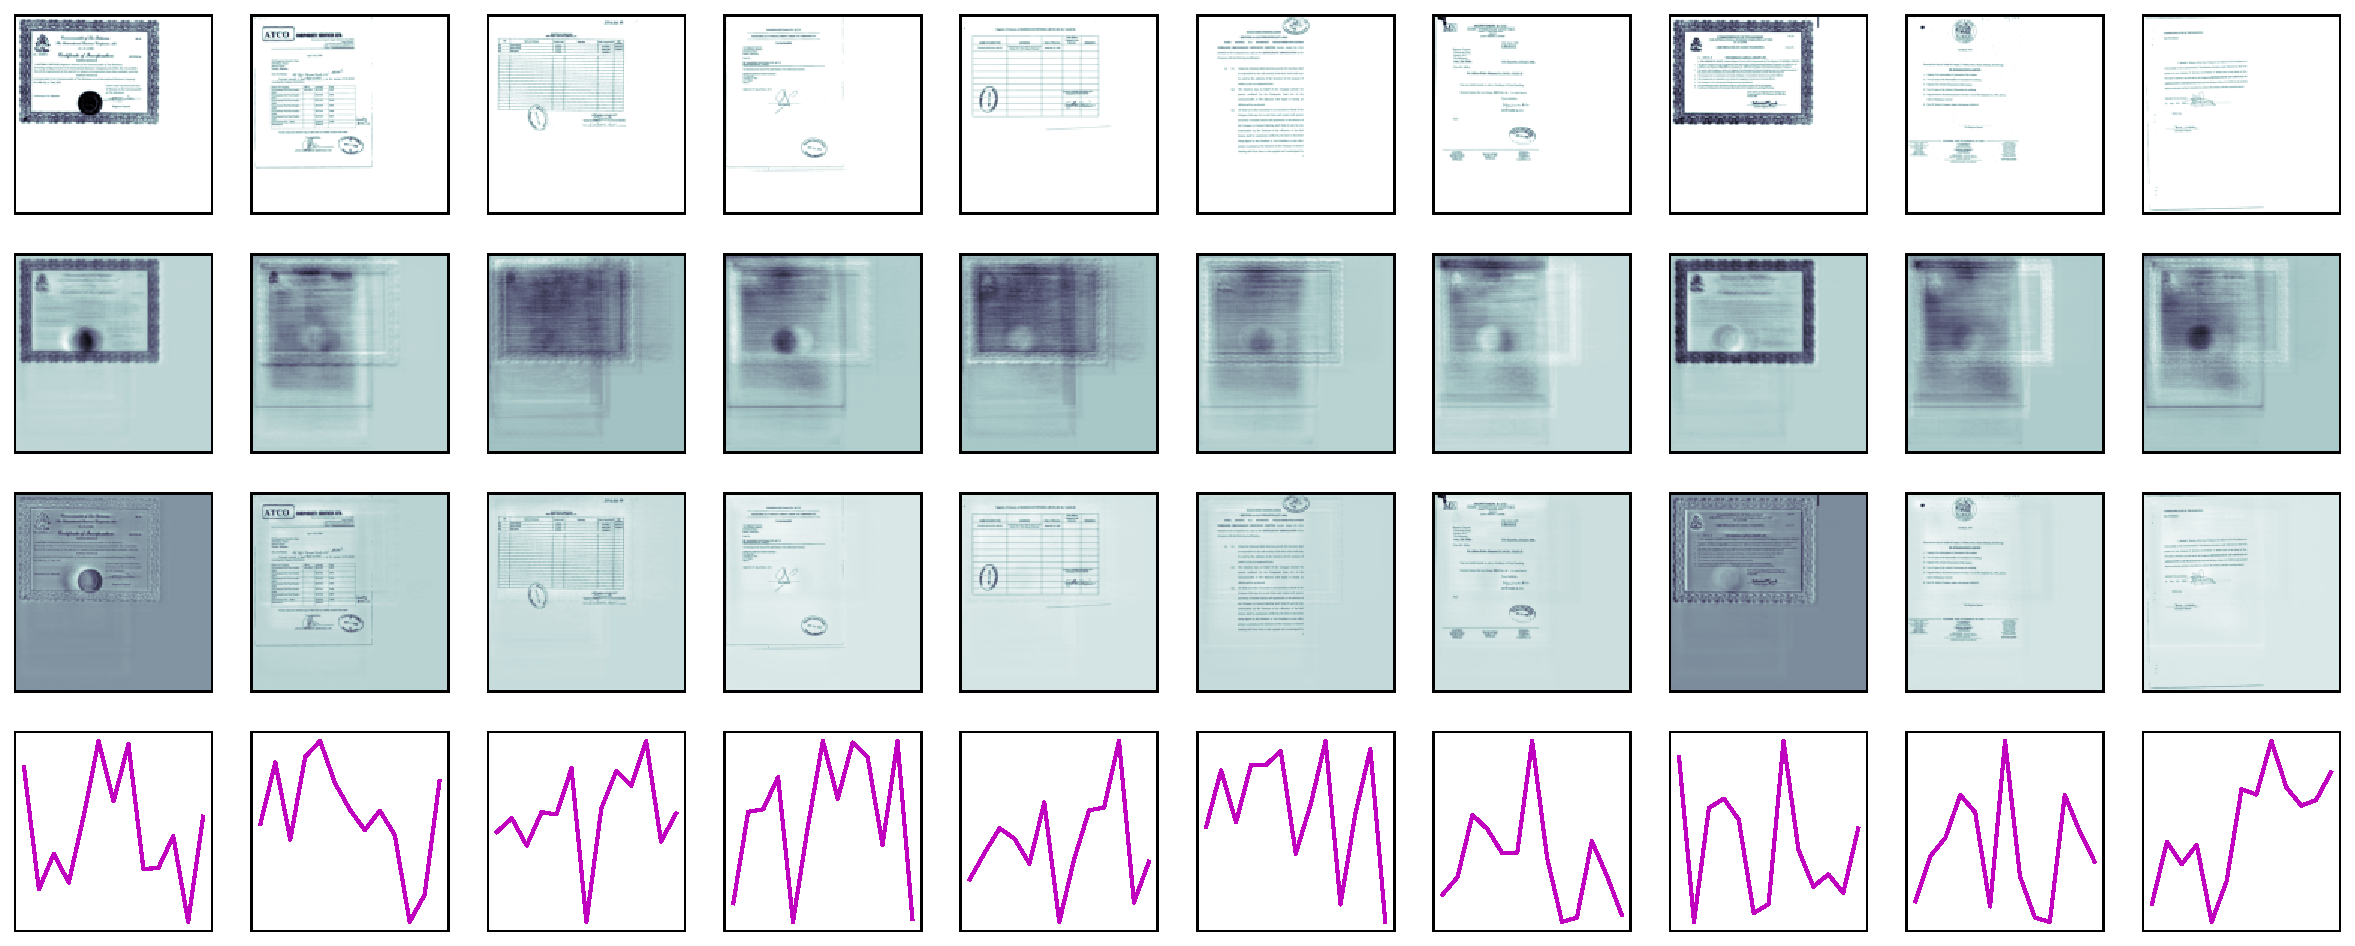
\includegraphics[width=1\textwidth]{images/Eigendocs/transformation/eigendocs.pdf}
    \caption[Preprocessing 10 randomly selected documents from the test set]{10 randomly selected documents from the test set.
    The number of images in the test set is 561, while the \ac{pca} model was fit to 1680 training images.
    The original images are displayed in the first row.
    The second row shows the reconstruction from their compressed version in the fourth row.
    The third row shows the reconstruction error, i.e. the difference between the reconstructed and the original image.
    The last row presents the greyscale values of the compressed 13-dimensional image as a line.
    }
    \label{fig:preprocessed_docs_eigendocs}
\end{figure}

The reachability distance ordered by \ac{optics} is displayed in \autoref{fig:reachability_plots}.
%The resulting clusters are displayed in \autoref{fig:optics_cluster}.

% reachability plot
\begin{figure}%
    \centering
    \subfloat[\centering The reachability plot of the documents preprocessed according to \autoref{pt:32} (cf. \cite{OPTICS1999}).]{{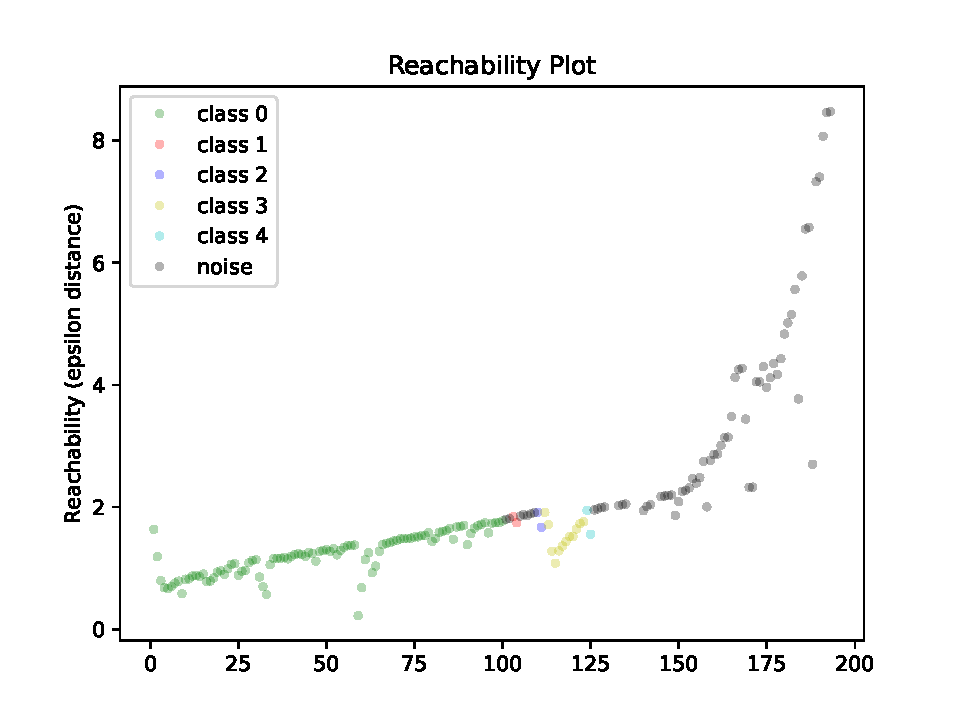
\includegraphics[width=5cm]{images/OPTICS/32x32/reachability_plot_32x32_pca_13dim.pdf} }}%
    \qquad
    \subfloat[\centering The reachability plot of the documents preprocessed according to \autoref{pt:eigendocs} (i.e. \eigendocs{}).]{{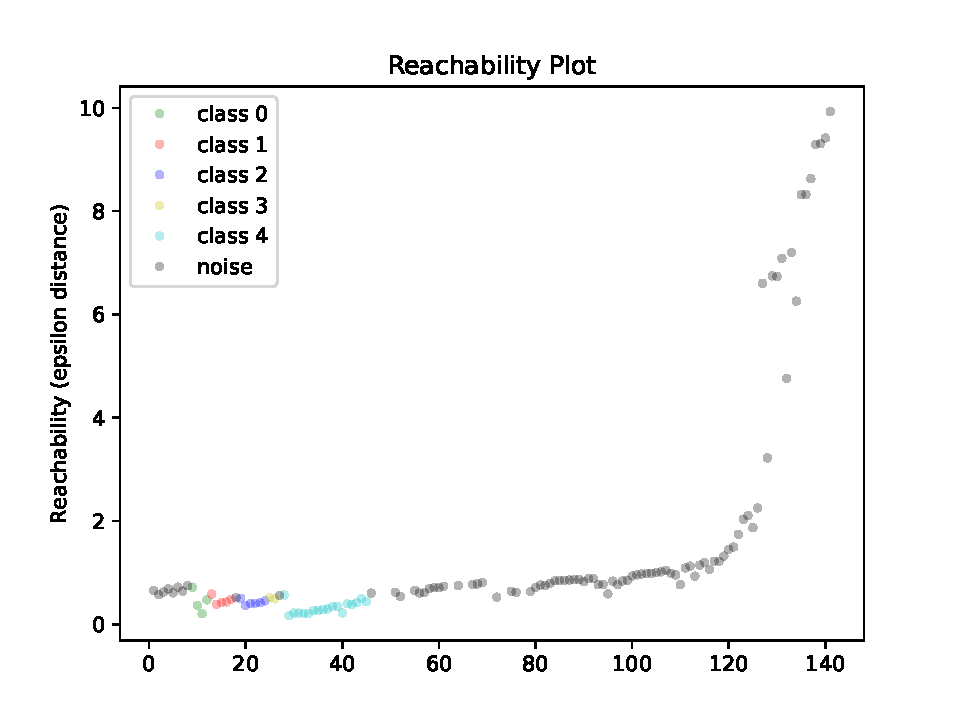
\includegraphics[width=5cm]{images/OPTICS/eigendocs/reachability_plot_13dim_eigendocs.pdf} }}%
    \caption[Reachability distances]{The plot was created using the \ac{optics} algorithm from the Python library scikit-learn.
    It shows the reachability distance of each document to its predecessor in the order list.}%
    \label{fig:reachability_plots}%
\end{figure}

% code
The configurations used when initializing an \ac{optics} model greatly influence the clusters returned.
The parameter \texttt{max\_eps} is infinity by default but can be specified by the user to reduce complexity and runtime.
According to literature, \texttt{max\_eps} should be big enough to include almost all points in a cluster.
The way the reachability plot is used to extract clusters is dependent on the \texttt{cluster\_method}. 
One can choose either \texttt{dbscan} or \texttt{xi} as a clustering method.
The parameters \texttt{min\_samples} and \texttt{eps} influence the cluster sizes and number of clusters found for a given clustering approach.
The value of \texttt{eps} defines the distance between two points to still be considered neighbours 
and can be chosen by consulting the reachability plot.
The code to initialize an exemplary \ac{optics} model is displayed in \lst{lst:optics_model}.

\begin{listing}[htp]
    \begin{minted}{python3}
        optics_model = OPTICS(cluster_method='dbscan', min_samples=2, max_eps=10, 
            eps=0.5)
    \end{minted}
    \caption[Initialization of the \ac{optics} model]{Initialization of the \ac{optics} model.
    The minimum number of samples \texttt{min\_samples} in a cluster corresponds to \textit{minPts}.
    }
    \label{lst:optics_model}
\end{listing}


% topic analysis
\subsection{Topic analysis}\label{impl-topic-modeling}

Two topic analysis approaches are outlined below.
The first one serves as the baseline model of this thesis and 
the second one is used multiple times throughout the application to visualize results obtained by queries.


\subsubsection*{\ac{t2v}}\label{subsubsec:impl-top2vec}

\citeauthor{Top2Vec2020}'s \ac{t2v} model is provided in the Python library \ac{t2v} \cite{Top2Vec2020}.
The non-changeable default values and settings of the model are listed below.
The word and document embeddings are generated by the \ac{d2v} version \ac{pvdbow}.
It has a window size of 15, uses hierarchical softmax, a minimum count of 50, a vector size of 300 and a sub-sampling threshold of $10^5$.
% dimensionality reduction
\ac{umap}'s hyperparameters are set to 15 nearest neighbours, cosine similarity as the distance metric and 5 as the embedding dimension in \citeauthor{Top2Vec2020}'s work.

In this work, a class is implemented, which uses the \ac{t2v} library.
When initiating an instance of this class, the \ac{t2v} model is trained on the given document corpus as displayed in \lst{lst:init-top2vec}.
The class provides methods to query for the number of topics as well as the 
most similar topics and documents to an input keyword.
The most similar topics can be visualized using \wordcloud{}s.
The core functionalities are implemented by the \ac{t2v} library, but the class is used to modify the return values to be compatible with the \ac{ui}.


\begin{listing}[htp]
    \begin{minted}{python3}
        Top2Vec(documents=self.documents, speed='fast-learn', workers=8)
    \end{minted}
    \caption[Initialization of the \ac{t2v} model]
    {Initialization of the \ac{t2v} model.
    }
    \label{lst:init-top2vec}
\end{listing}

\section{\wordcloud{}}\label{sec:impl-wordcloud}

The implementation of \wordcloud{}s in this thesis is based on the Python library \textit{wordcloud} \cite{wordcloud-dev}.
This implementation removes English stop words from the text by default.
The input text is split into tokens using a regex.
By default, plurals are removed if their singular version is present and their frequency is added to their singular version.
By default, numbers are not included as tokens.

% custom preprocessing
In order to ensure that the words presented are interpretable, the input text is preprocessed.
A lemmatizer is used to ensure stemmed words exist.
The lemmatizer used is \texttt{WordNetLemmatizer} from the \texttt{nltk} package as displayed in \lst{lst:impl-preproc-wordcloud}.

% initialization
The \wordcloud{} is initialized as shown in \lst{lst:impl-wordcloud}.

\begin{listing}[htp]
    \begin{minted}{python3}
        lemmatizer = WordNetLemmatizer()
        tokens = [lemmatizer.lemmatize(token) for token in tokens]
    \end{minted}
    \caption[Custom preprocessing of \wordcloud{} input]
    {Custom preprocessing of \wordcloud{} input.
    }
    \label{lst:impl-preproc-wordcloud}
\end{listing}

\begin{listing}[htp]
    \begin{minted}{python3}
        wordcloud = WordCloud(width=800, height=500, random_state=21, 
            contour_width=3, max_font_size=110, background_color='white', 
            max_words=5000).generate(','.join(tokens))
    \end{minted}
    \caption[Initialization of the \wordcloud{}]
    {Initialization of the \wordcloud{}.
    }
    \label{lst:impl-wordcloud}
\end{listing}



% Slurm/ Server

\subsection{\slurm{}}\label{subsec:slurm}

Since the data corpus is too big to be processed locally on a \localMaschineStats{}, the Chair \ac{ies} has offered to provide computational means to solve this problem.
The scripts can be processed by multiple nodes which are managed by \slurm{}.

\slurm{} is an open-source management tool for Linux clusters \cite{slurm-online}.
It allocates resources, i.e.\ compute nodes, and provides the means to start, execute and monitor jobs \cite{slurm-online, slurm2003}.

The so-called \slurm{} daemons control nodes, partitions, jobs and job steps \cite{slurm-online}.
A partition is a group of nodes and a job is the allocation of resources, i.e.\ compute nodes, to a user for a limited period of time.
A basic visualization of the architecture is given in \autoref{fig:slurm-architecture}.

\begin{figure}[!htb] % htp = hier (h), top (t), oder auf einer eigenen Seite (p).
    \centering
    \includesvg[width=0.7\textwidth]{images/slurm/slurm_architecture}
    \caption[\slurm{} architecture]{\slurm{} architecture. The management node has a \texttt{slurmctld} daemon, while every compute node has a \texttt{slurmd} daemon.
    The nodes communicate.
    The user can use certain commands, for instance \texttt{srun} and \texttt{squeue}, anywhere on the cluster.
    }
    \label{fig:slurm-architecture}
\end{figure}

% sbatch scripts
A job is started by a \texttt{sbatch} script.
This script defines the \texttt{partition}, the \texttt{job-name}, the number of \texttt{nodes}, the \texttt{cpus-per-task}, the memory \texttt{mem} allocated, 
the \texttt{time} limit and the path to store \texttt{error} and \texttt{output} logs.
It is possible to work on multiple \acp{cpu} simultaneously to divide the workload of a task.
In this work, multiple \texttt{sbatch} scripts are used to carry out a variety of tasks.
A summary of the tasks and scripts is given in \autoref{tbl:sbatch-scripts}.


\begin{table}[]
    \caption{A selection of \texttt{sbatch} scripts used in this work.}
    \begin{tabular}{|
    >{\columncolor[HTML]{EFEFEF}}p{0.28\textwidth} |p{0.68\textwidth}|}
    \hline
    \cellcolor[HTML]{C0C0C0}\textbf{Name of sbatch script} & \cellcolor[HTML]{C0C0C0}\textbf{Description}                                                                                                                                                                                                                      \\ \hline
    ae\_config.sh                                          & Comparison of different \ac{ae} architectures in terms of the metrics cosine similarity and \ac{rsme}.                                                                                                                                                                     \\ \hline
    allocate\_res.sh                                       & Allocates resources to enable a \ac{ssh} tunnel connection from a local \ac{vscode} instance to the server of the \ac{ies}. 
                                                                When enabled, the database content can be displayed with the \databaseName{} plugin.\\ \hline
    create\_database.sh                                    & Initializes the database by specifying fields.                                                                                                                                                                                                                    \\ \hline
    create\_documents.sh                                   & Inserts the document's metadata information, i.e.\ path and text.                                                                                                                                                                                                   \\ \hline
    elasticContainer.sh                                    & Starts the \databaseName{} container using the headless \texttt{podman-compose up} command.                                                                                                                                     \\ \hline
    init\_database.sh                                      & Initializes database, subsequentially inserts documents metadata, embeddings and clusters.                                                                                                                                                                        \\ \hline
    insert\_clusters.sh                                    & Inserts \ac{pca} weights, \ac{optics} and argmax clusters.                                                                                                                                                                      \\ \hline
    insert\_embeddings.sh                                  & Subsequentially inserts embeddings of documents.                                                                                                                                                                                                                  \\ \hline
    own\_w2v\_model.sh                                     & Creates and saves custom \ac{w2v} model.                                                                                                                                                                                                          \\ \hline
    run\_pdf2png.sh                                        & Converts and saves the \ac{png} version of the first page of the \acp{pdf}.                                                                                                                                                             \\ \hline
    \end{tabular}
    \label{tbl:sbatch-scripts}
\end{table} % last subsection

% UI
\section{\acl{ui}}\label{sec:ui}

Since this work should be valuable to (German) tax offices, a basic \ac{ui} is provided.
However, the focus of this work is on the methods and not on the \ac{ui}.
The \ac{ui} is divided into two parts, the frontend and the backend.

\subsection{Backend}\label{subsec:backend}

% this work: endpoints
The framework used for the backend is \flask{}.
In this work, only the \texttt{GET} method is used.
There are multiple endpoints, which are used to retrieve data from the server:

\begin{itemize}
    \item \label{pt:docs}Documents: 
        Returns a list of documents, which best match the query.
        The query can be of type \texttt{match\_all}, which returns all documents in the database, 
        or a fuzzy full-text query, 
        or a \ac{knn} query on a certain field of the database.
        Moreover, the number and start index of the results returned can be specified.

    \item \label{pt:doc}Document: 
        Returns the document with the specified \texttt{id}.

    \item \label{pt:pdf}\ac{pdf}: 
        Returns the path to a \ac{pdf} file.
        In order to access the path information a query for a document with the specified \texttt{id} is performed.
    
    \item \label{pt:wordcloud}WordCloud: 
        Returns the bytes of a WordCloud image. 
        Depending on additional parameters, the WordCloud is either generated from one document or 
        the most similar documents to the query field, identified by \ac{knn}.

    \item \label{pt:termfrequency}Term Frequency:
        Returns the term frequency calculated for the specified document.
\end{itemize}

In order to test the endpoints during development, swagger documentation for every endpoint is provided.





\subsection{Frontend}\label{subsec:frontend}

The framework used for the frontend is \angular{}.
There are three main components, which are used to display the data:

\begin{itemize}
    \item \label{pt:home}Home: 
        The home component is used to display the results of a query.
        It consists of a search bar, which is used to enter the text query, and a list of results.
        If no text query is entered the first documents of the database, i.e. the result of a \texttt{match\_all} query, are displayed.
        The search component is shown in \autoref{fig:home_comp}.

    \item \label{pt:detail}Detail: 
        The detail component is used to display the details of a document.
        The document name and ID are located on the left side of the screen.
        Beneath the document name and ID, a button which opens the term frequency image on a new page upon pressing is located. 
        Moreover, the WordCloud of the document is displayed.
        The WordCloud is generated from the text of the document.
        On the right side of the screen, there is a \ac{pdf} viewer which displays the pages of the document.
        Beneath the \ac{pdf} viewer, the names and WordClouds of the most similar documents are displayed after a query for them is initiated by the user.
        The detail component is shown in \autoref{fig:detail_comp}.

    \item \label{pt:topic}Topic: 
        The topic component is used to display the topics of the documents.
        The topics are generated by \texttt{top2vec}.
        The topic component is shown in \autoref{fig:top2vec_topic_comp}.
\end{itemize}


\begin{figure}[htp] % htp = hier (h), top (t), oder auf einer eigenen Seite (p).
    \centering
    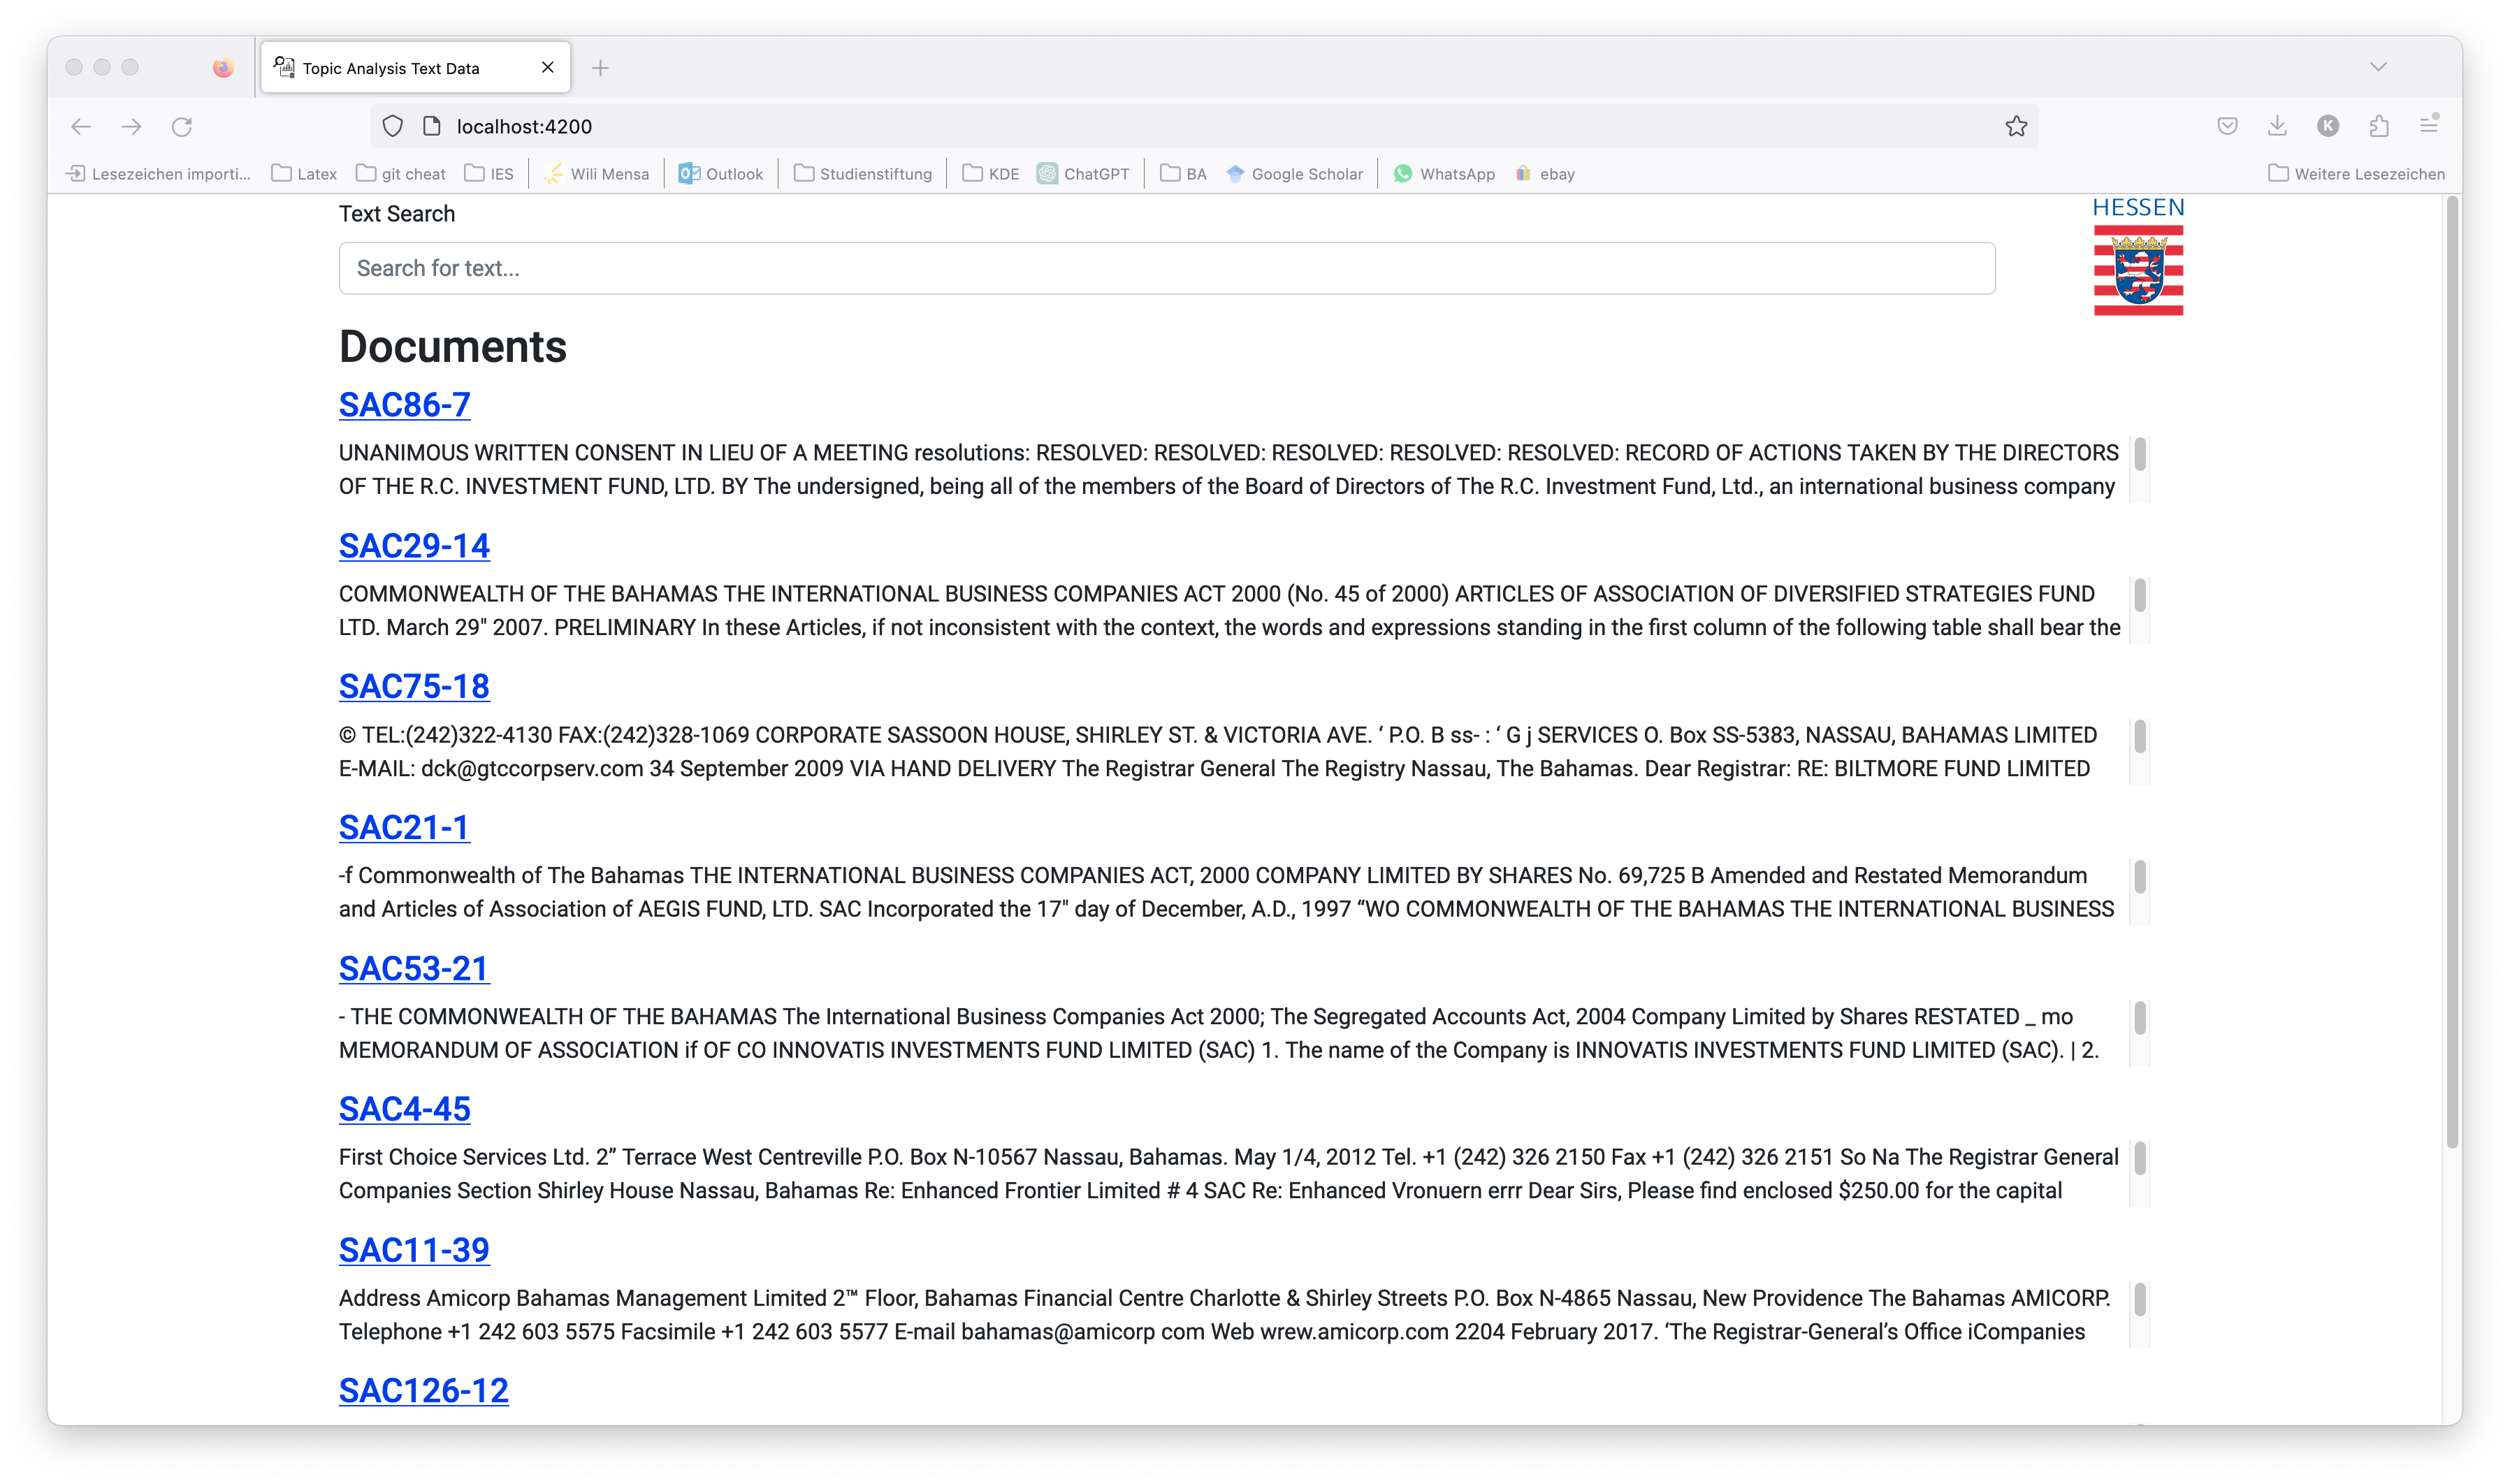
\includegraphics[width=0.7\textwidth]{images/UI/Home_component.png}
    \caption{Home component of the frontend.
    The search bar is used to enter the text query.
    The results of the query are displayed below the search bar.
    }
    \label{fig:home_comp}
\end{figure}


\begin{figure}[htp] % htp = hier (h), top (t), oder auf einer eigenen Seite (p).
    \centering
    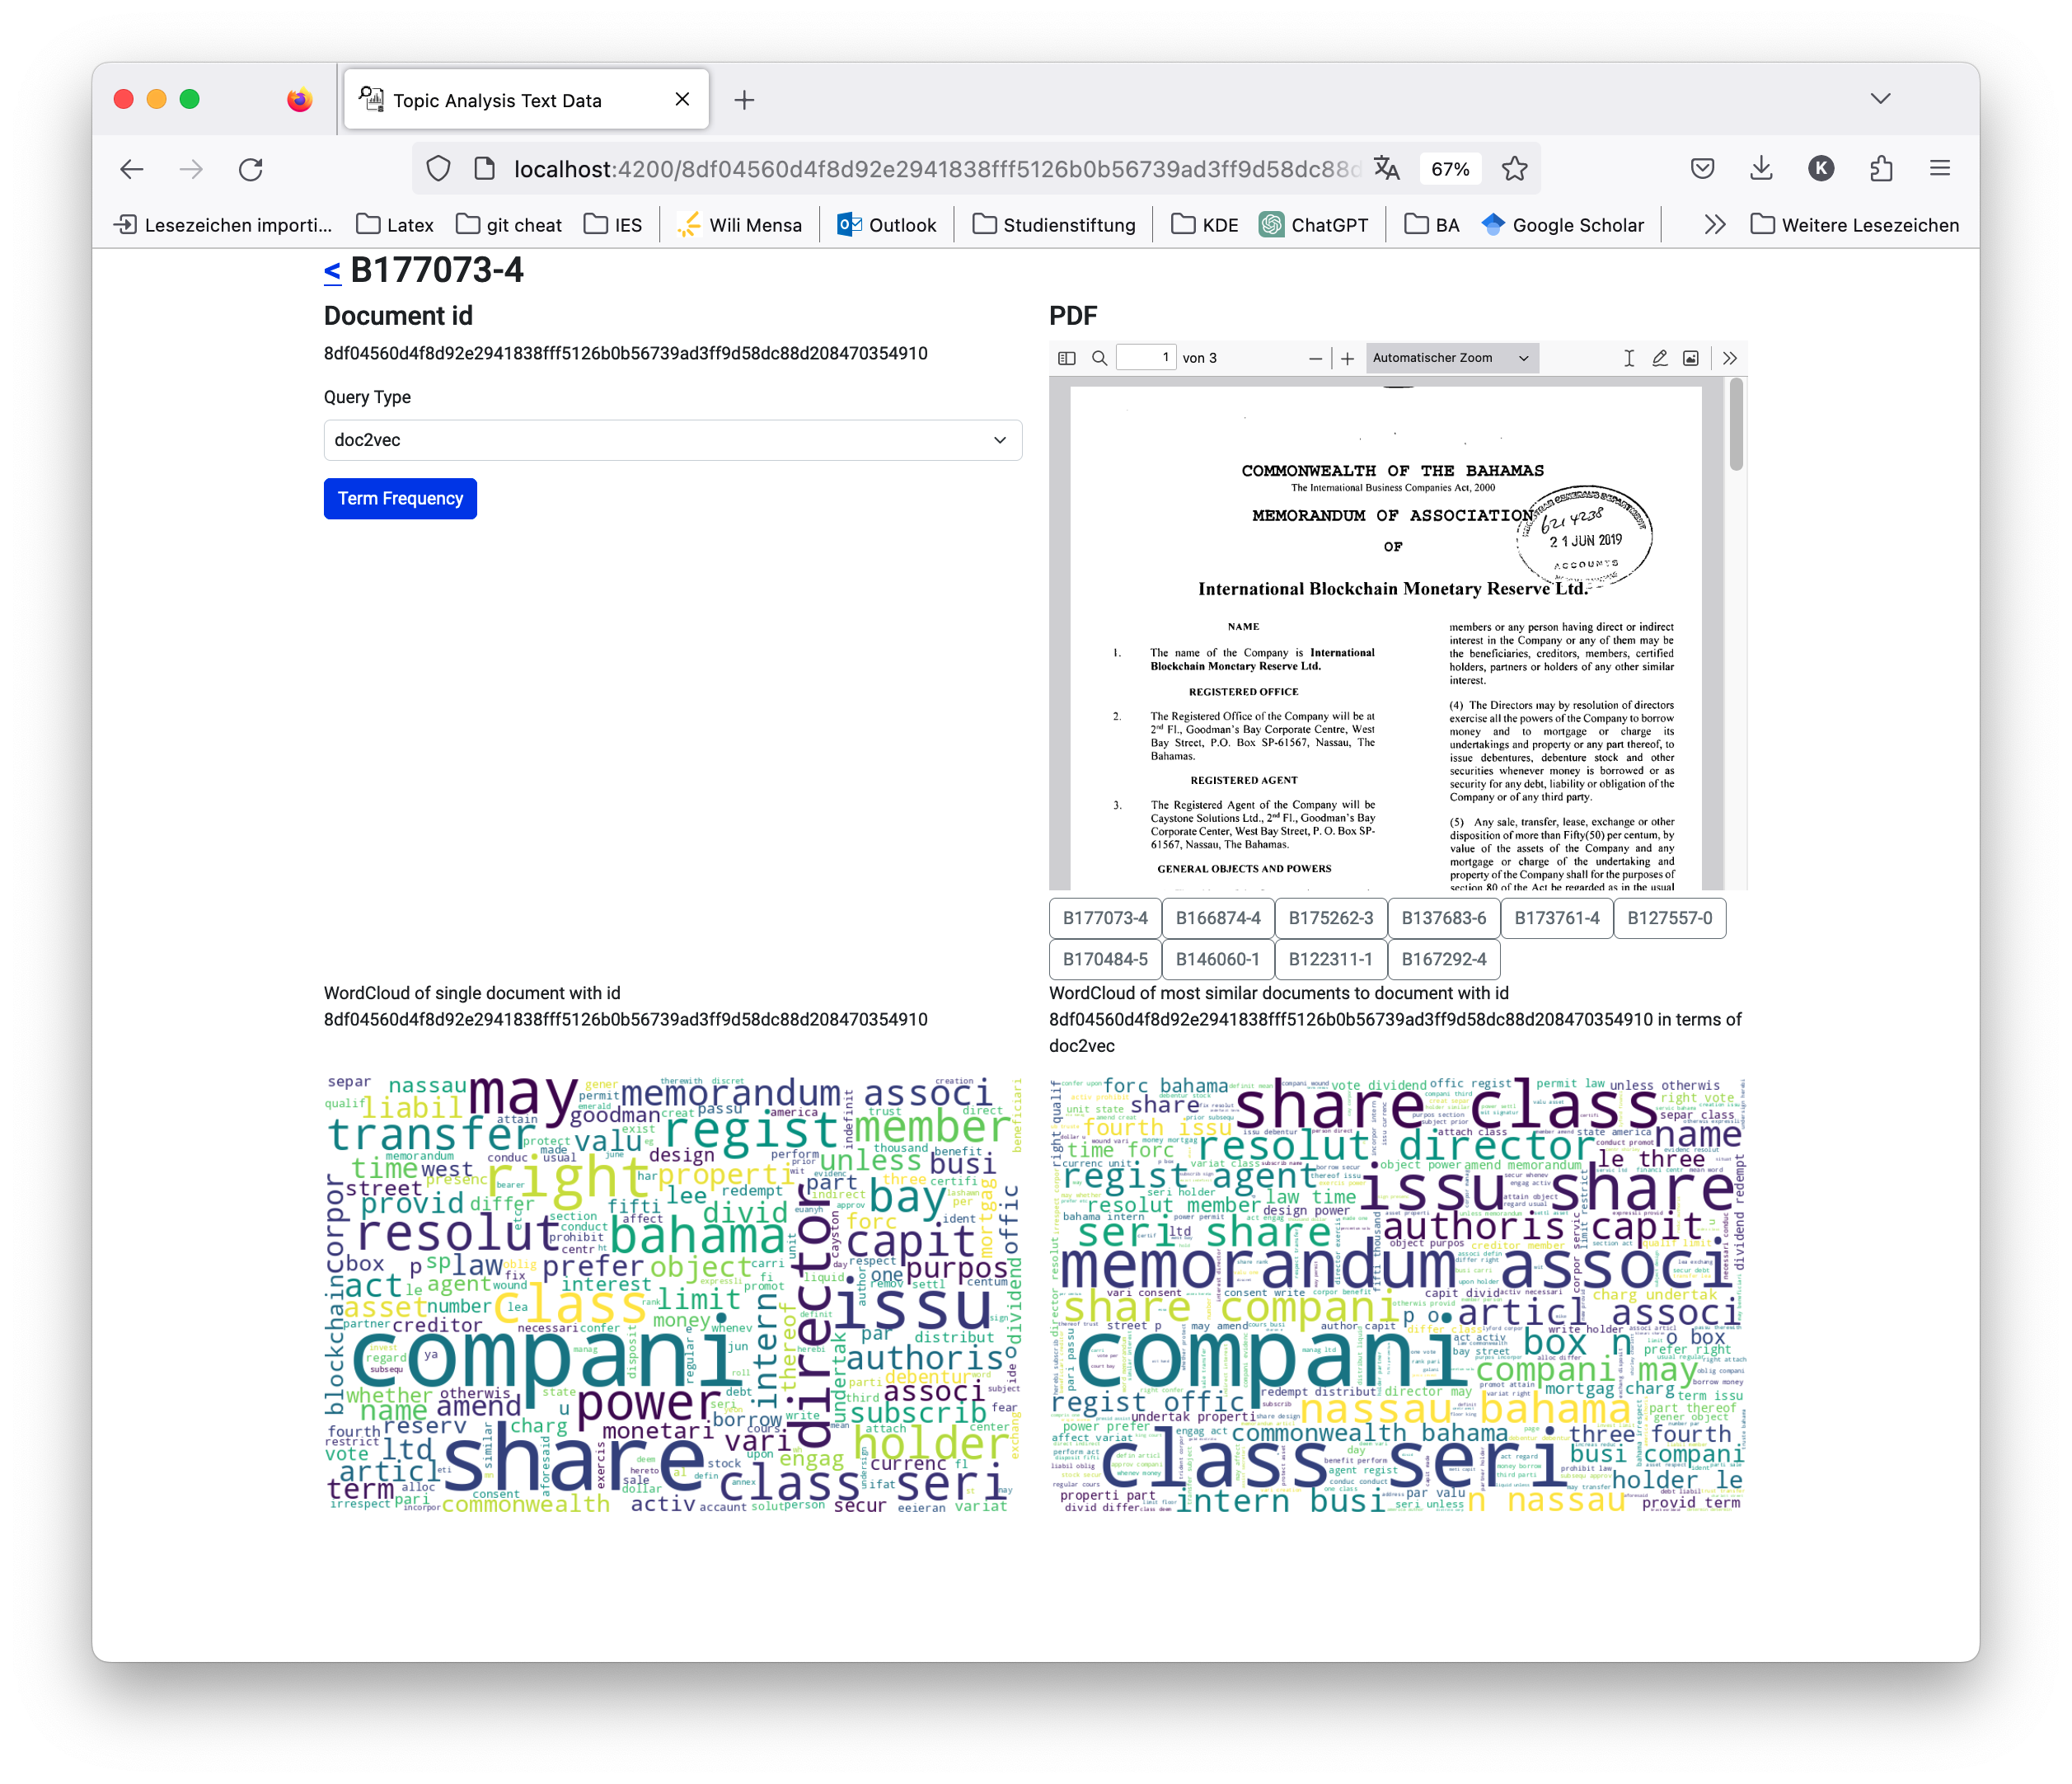
\includegraphics[width=0.7\textwidth]{images/UI/Home_detail.png}
    \caption{Detail component of the frontend.
    The chosen document is displayed, as well as its most similar documents in the database.
    WordClouds of the document and the most similar documents are displayed.
    }
    \label{fig:detail_comp}
\end{figure}


\begin{figure}[htp] % htp = hier (h), top (t), oder auf einer eigenen Seite (p).
    \centering
    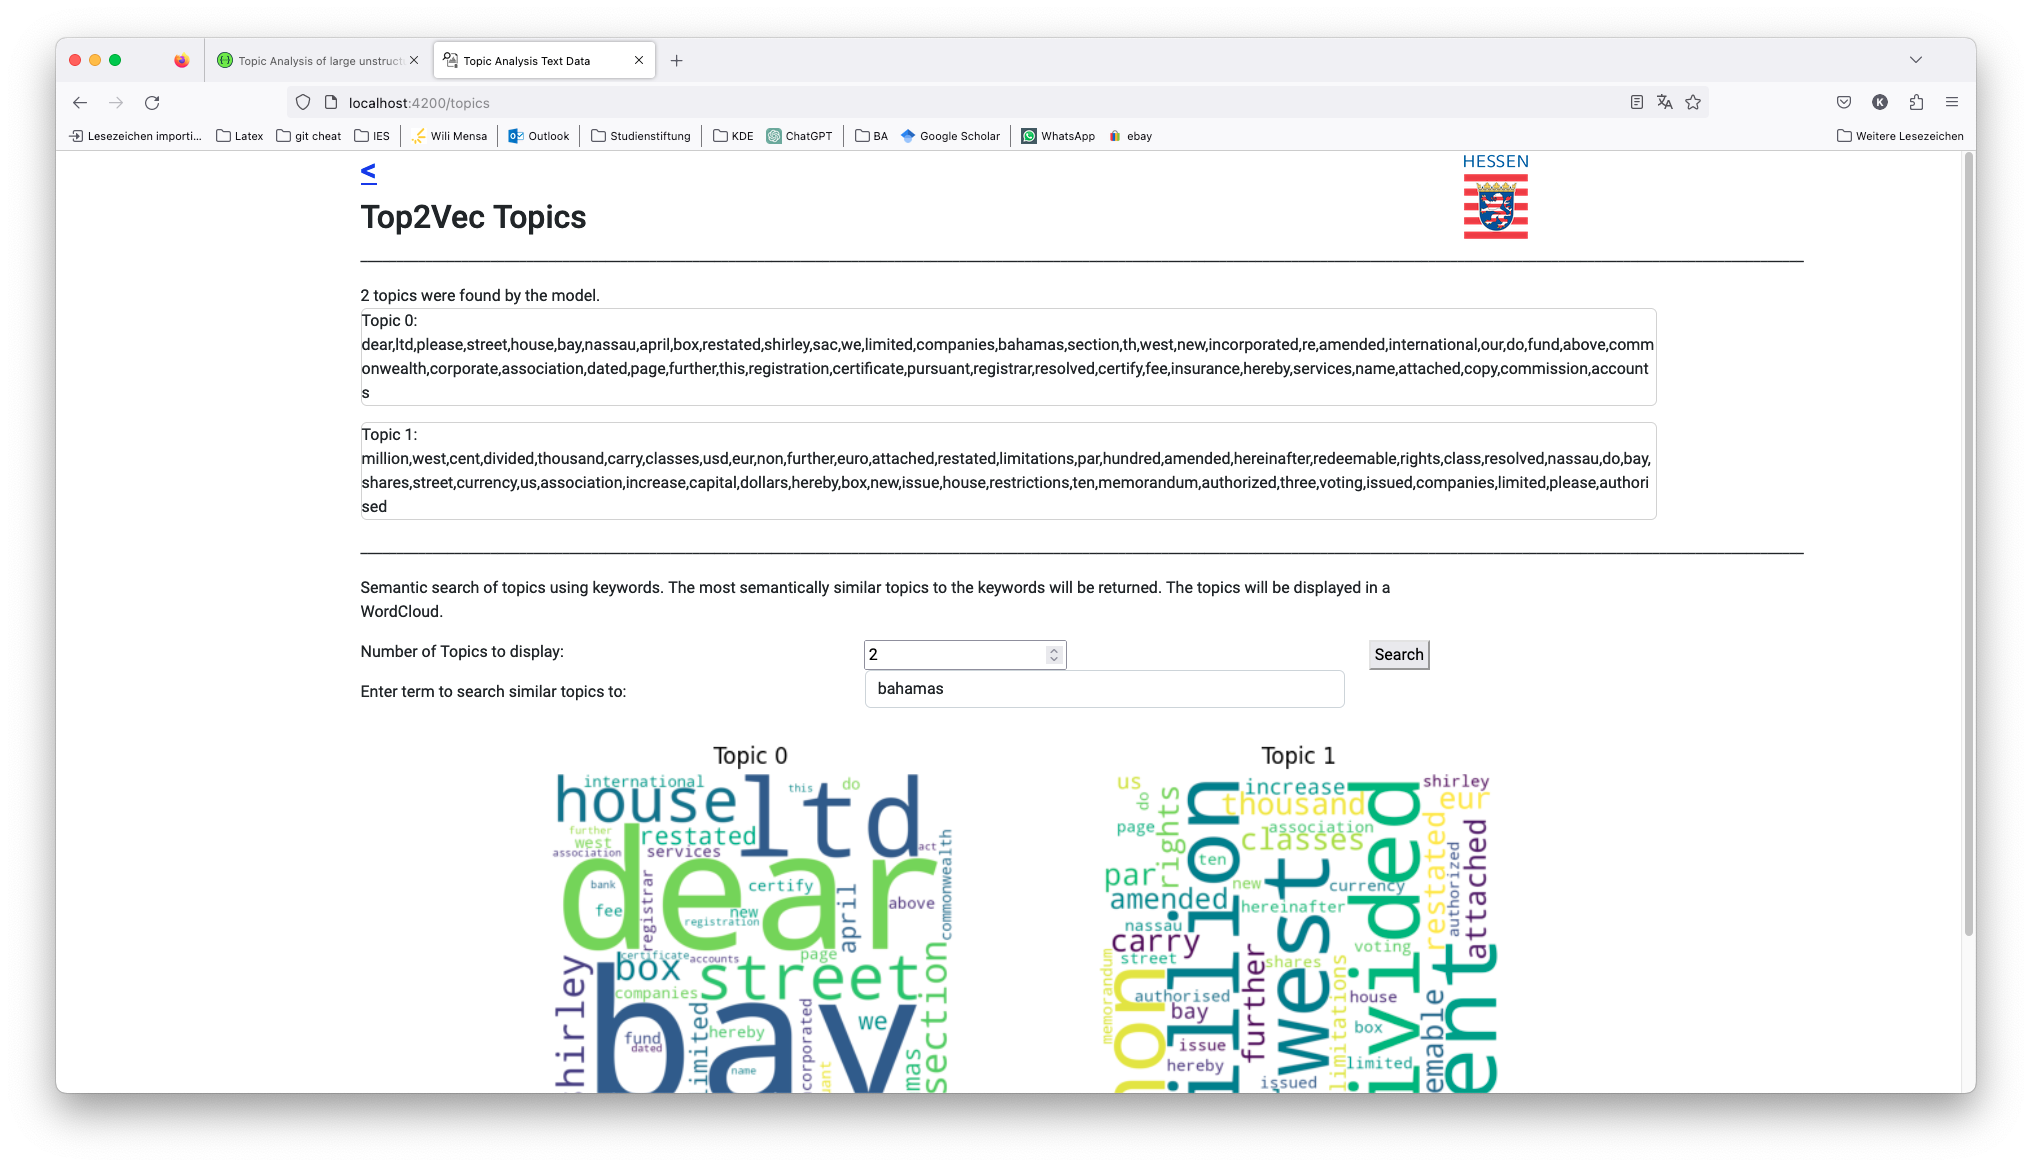
\includegraphics[width=0.7\textwidth]{images/UI/Top2Vec_Topics.png}
    \caption{Topic component of the frontend.
    }
    \label{fig:top2vec_topic_comp}
\end{figure}


To change between the components, the routes have to be defined.
The routes are defined in the \texttt{app-routing.module.ts} file, as shown in \autoref{lst:angular_routing}.

\begin{listing}[htp]
    \begin{minted}{typescript}
        const routes: Routes = [
            { path: ':id', component: DocumentDetailComponent},
            { path: '', component: HomeComponent},
          ];
    \end{minted}
    \caption{Definition of routes in \angular{} in the app-routing.module.ts.
    }
    \label{lst:angular_routing}
\end{listing}


\section{Trade-off between memory and query time}\label{sec:trade-off}

At the beginning of this thesis, it was unclear to what degree the tool, 
i.e.\ the database fields and query results should be precomputed.
A tool which is trained once offline is beneficial due to the amount of data.
Since \databaseName{} provides fast queries, it is sufficient to rely on real-time queries.

In the course of filling the database with information, 
one had to face obstacles not only regarding excessive memory usage but also long run times of methods.
Early on it became evident that one either had to reduce accuracy and details in order to achieve less memory or 
one had to settle for minutes to hours of calculations and bigger costs in terms of memory consumption.

Beforehand, it was not as clear which information, i.e.\ fields in the database, seemed worth the time and memory.
For instance, initially, the image of the first \ac{pdf} page of each document was saved alongside the other fields within the database.
After scaling the amount of data stored in the database to about 2900 documents, 
this approach caused severe issues in terms of memory usage.
Hence, this field is omitted.
    \chapter{Evaluation}\label{ch:evaluation}

Since the dataset has no ground truth, the procedure used to pick the parameter values is not comparable to ground truth-based approaches.
Hence, the evaluation is informal and the methods applied have arisen from regular consultation with experts from the tax office.
Run times of different configurations are measured and compared.
Parameters are chosen with respect to model-specific procedures, such as reachability plots for \ac{optics}.
The models are compared to each other and their composition to the baseline topic analysis model \ac{t2v}.


 % Database
 \section{Database}\label{sec:eval-db}
There is a variety of parameter values to choose from when working with databases and embeddings.
These parameters include similarity metrics and the choice of query types.

 \subsection*{Similarity measurements}\label{subsec:evaluation-sim-measurements}

According to \citeauthor{HfsentTrans2019}, the similarity measurements discussed in \autoref{sec:similarity-measurement} 
obtained roughly the same results in their experiments \cite{HfsentTrans2019}.   

% similarity
As the similarity between vectors is usually calculated using some form of cosine similarity, 
rather than Euclidean distance in literature, cosine is preferred over Euclidean distance. 
Since the models may produce embeddings, which are not normalized, the cosine similarity is used instead of the dot product.
Soft cosine similarity is not used, since it is not available in \databaseName{}.
However, the usage of soft cosine would likely improve the results.

 \subsection*{\databaseName{}}\label{subsec:evaluation-db}
% SQL vs NoSQL
According to \citeauthor{flask_book2018}, \ac{sql} databases are a good choice for efficiently storing structured data.
This is because their paradigm \acs{acid}, i.e. \acl{acid}, provides high reliability.
\ac{nosql} databases, on the other hand, are more flexible and can be used to store unstructured data \cite{flask_book2018}.
They do not require a predefined schema and can therefore accept documents of arbitrary structure \cite{flask2018}.
Usually, \ac{nosql} databases do not offer services such as \texttt{JOIN} \cite{flask2018}.
%According to \citeauthor{flask2018}, \ac{nosql} databases make a tradeoff between storage and speed, as well as a tradeoff between consistency and availability.
\ac{nosql} databases are said to outperform out-of-the-box \ac{sql} databases \cite{flask2018}.
Since the dataset consists of unstructured documents and the task at hand does not require performing any \texttt{JOIN}s a \ac{nosql} database is favourable.
\databaseName{} was chosen since it is well known to provide near real-time search and to operate on big data.
Subsequently, it is a good fit for the underlying dataset.

% separation of initialisation and insertion
The time necessary to perform the steps of filling the \databaseName{} database has been evaluated and improved throughout this work.
The current time measurements are shown in \autoref{fig:time_init_db}.
Portioning the work with the database is beneficial since it is possible to update the embeddings without having to recreate the database.
Moreover, modulizing the initialization and filling of the database facilitates debugging and comparing the models used to create the embeddings.

\begin{figure}[htp] % htp = hier (h), top (t), oder auf einer eigenen Seite (p).
    \centering
    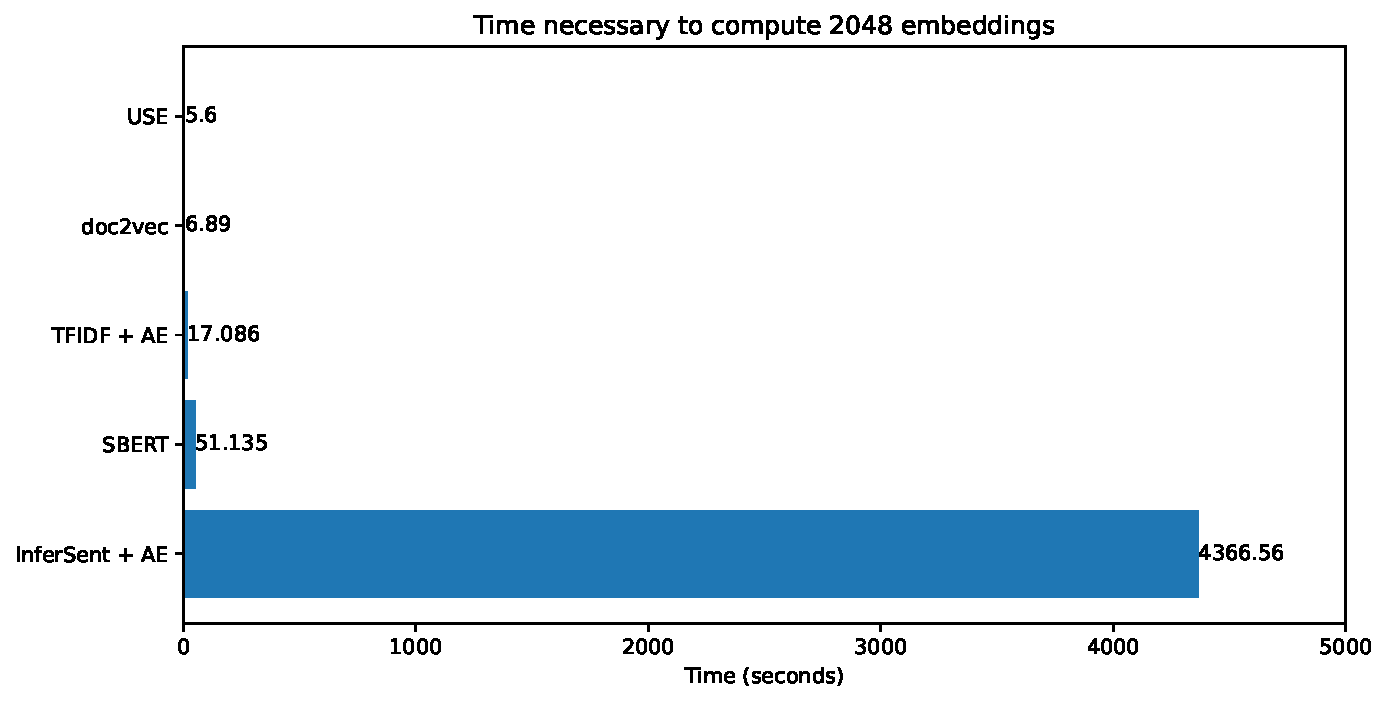
\includegraphics[width=0.6\textwidth]{images/Elasticsearch/Time_necessary_to_compute_2048_embeddings.pdf}
    \caption[Times for creating the database]{Time per module of creating the Bahamas database using a random selection of 2048 documents.
    The reference time was measured using \texttt{cProfiler} on a \localMaschineStats{}.
    %the \texttt{timer} from \texttt{timeit.default\_timer} on a \localMaschineStats{}.
    }
    \label{fig:time_init_db}
\end{figure}

%A document store database can be used if the primary goal is to write fast rather than write save \cite{flask2018}.

 % Eigendocs
 \section{\eigendocs{}}\label{sec:evaluation-eigendocs}
% idea 
% Assuming the layout holds information about the document type, the first page of each document is used to extract this information.
% In the course of working with low-quality versions of the documents to minimize the memory necessary to store them, some documents looked similar.
% Therefore, the idea arose to use clustering algorithms to group the documents according to their appearance.

% number of components
In order to determine the optimal number of components used for \eigendocs{} the cumulative explained variance and the reconstruction error are plotted 
as displayed in \autoref{fig:det_n_comp} from \autoref{subsec:eigenface}.
The first plot indicates that 90\% of the variance is explained by 441 components.
Usually, that would have been the number of dimensions of the subspace onto which the documents would have been projected.
However, when working with clustering algorithms like \ac{optics}, the number of dimensions should be reduced even further to achieve valid clusters.
Therefore the reconstruction error with respect to different numbers of components is taken into consideration.

\begin{listing}[htp]
    \begin{minted}{python3}
        sqr_dif = (X_test - X_test_pca_inverse)**2
        reconstr_err.append(np.sqrt(np.mean(sqr_dif))/
            (np.sum(np.abs(1-X_test))/X_test.shape[0])) 
    \end{minted}
    \caption[Adaption of the \ac{rsme}]{
        Adaption of the \ac{rsme}: 
        Firstly, the squared differences between the original and the reconstructed images are calculated.
        Since the values are normalized, a 1 corresponds to a white pixel.
        Then, the absolute values of all non-white pixels of the test set are summed up.
        The average number of non-white pixels is calculated by dividing the sum by the number of images in the test set.
        This approach considers pixels of value $p \in [0,1]$ as $(p \cdot 100)$\% white and thus, they are incorporated in the sum.
    }
    \label{lst:impl-weighted-rsme}
\end{listing}

Usually, a \ac{rsme} is minimized to determine the optimal parameter configurations.
In this case, the reconstruction error shall be interpreted.
To facilitate the interpretability of the reconstruction error, its calculation is adapted to incorporate the content of the images.
At first sight, the majority of image pixels are white, i.e.\ do not convey any information.
Therefore, the reconstruction error is divided by the average number of non-white pixels. 
Hence, the reconstruction error of an image is weighted by the amount of information it conveys.
The calculation is given in \lst{lst:impl-weighted-rsme}.
The result is displayed in \autoref{fig:det_n_comp}.
Since the reconstruction error increases less rapidly after 10 to 20 components, the number of components is set to 13,
which has been an "elbow" point in a similar trial using a not randomly selected dataset of 195 images.


% results
Some impressions of the \eigendocs{} algorithm are displayed in \autoref{fig:preprocessed_docs_eigendocs}.
Assuming that the selection of documents is representative, 
the preprocessing of the documents using \eigendocs{} should have encoded information about the dimensionality of the images.
However, this assumption is not valid since bigger images exist.
Therefore, the idea of incorporating information about the image's dimensions is not entirely implemented.
 
 % Embeddings
\section{Embeddings}\label{sec:eval-embeddings}
As discussed in \autoref{subsec:impl-embeddings}, there is a range of possible parameter values to choose from when implementing embedding models.
The section below states which findings have led to the parameter values applied in this work.

\subsection*{\acs{tfidf}}\label{subsec:evaluation-tfidf}

The main obstacle to overcome is the high dimensionality of the \ac{tfidf} embeddings.
Hence, the goal of the parameter selection is to find a way to reduce the dimensionality of the vocabulary to 2048 
which is the maximum vector dimensionality of \databaseName{}.
However, the quality of the embeddings should not decline too much.

% parameter selection
The choice of the preprocessor is investigated with regard to the goal of minimizing the vocabulary size.
Both the default and a custom preprocessor are tested on a data corpus of 2048 randomly selected documents concerning the vocabulary (size).
While the default preprocessor had a vocabulary size of 5893, the custom preprocessor had a size of 5585.
The relative difference likely shrinks with a larger data set, 
since the trend is already visible for two different data corpus sizes in \autoref{tab:tfidf-preprocessor-comparison}.
The custom preprocessor is chosen because it had a smaller vocabulary size.
The differences between both vocabularies are visualized in \autoref{fig:differences-vocabularies}.

As stated in \autoref{sec:eval-db}, the \ac{tfidf} embeddings can be problematic 
with regard to the maximal dimensionality of dense vectors stored in \databaseName{}.
Hence, this work has to employ dimensionality reduction techniques to reduce the dimensionality of the embeddings.


% Please add the following required packages to your document preamble:
% \usepackage[table,xcdraw]{xcolor}
% Beamer presentation requires \usepackage{colortbl} instead of \usepackage[table,xcdraw]{xcolor}
\begin{table}[]
    \caption[Comparison of the default and the custom \ac{tfidf} preprocessor]
    {Comparison of vocabulary sizes resulting from the default and the custom \ac{tfidf} preprocessor on different data corpus sizes.}
    \begin{tabular}{|p{0.55\textwidth}|p{0.2\textwidth}|p{0.2\textwidth}|}
    \hline
                                                                                                    & \cellcolor[HTML]{C0C0C0}{\color[HTML]{000000} \textbf{first trial}} & \cellcolor[HTML]{C0C0C0}{\color[HTML]{000000} \textbf{second trial}} \\ \hline
    \cellcolor[HTML]{C0C0C0}{\color[HTML]{000000} \textbf{document corpus size M}}                 & {\color[HTML]{000000} 195}                                          & {\color[HTML]{000000} 2048}                                          \\ \hline
    \cellcolor[HTML]{C0C0C0}{\color[HTML]{000000} \textbf{custom preprocessor vocabulary size A}}  & {\color[HTML]{000000} 1521}                                         & {\color[HTML]{000000} 5585}                                          \\ \hline
    \cellcolor[HTML]{C0C0C0}{\color[HTML]{000000} \textbf{default preprocessor vocabulary size B}} & {\color[HTML]{000000} 1641}                                         & {\color[HTML]{000000} 5893}                                          \\ \hline
    \cellcolor[HTML]{C0C0C0}{\color[HTML]{000000} \textbf{(B-A)/M}}                                & {\color[HTML]{000000} 120/195 = 0,6153846154}                       & {\color[HTML]{000000} 308/2048 = 0,150390625}                        \\ \hline
    \end{tabular}
    \label{tab:tfidf-preprocessor-comparison}
\end{table}

\begin{figure}%
    \centering
    \subfloat[\centering The terms only present in the vocabulary produced by the default preprocessor.]{{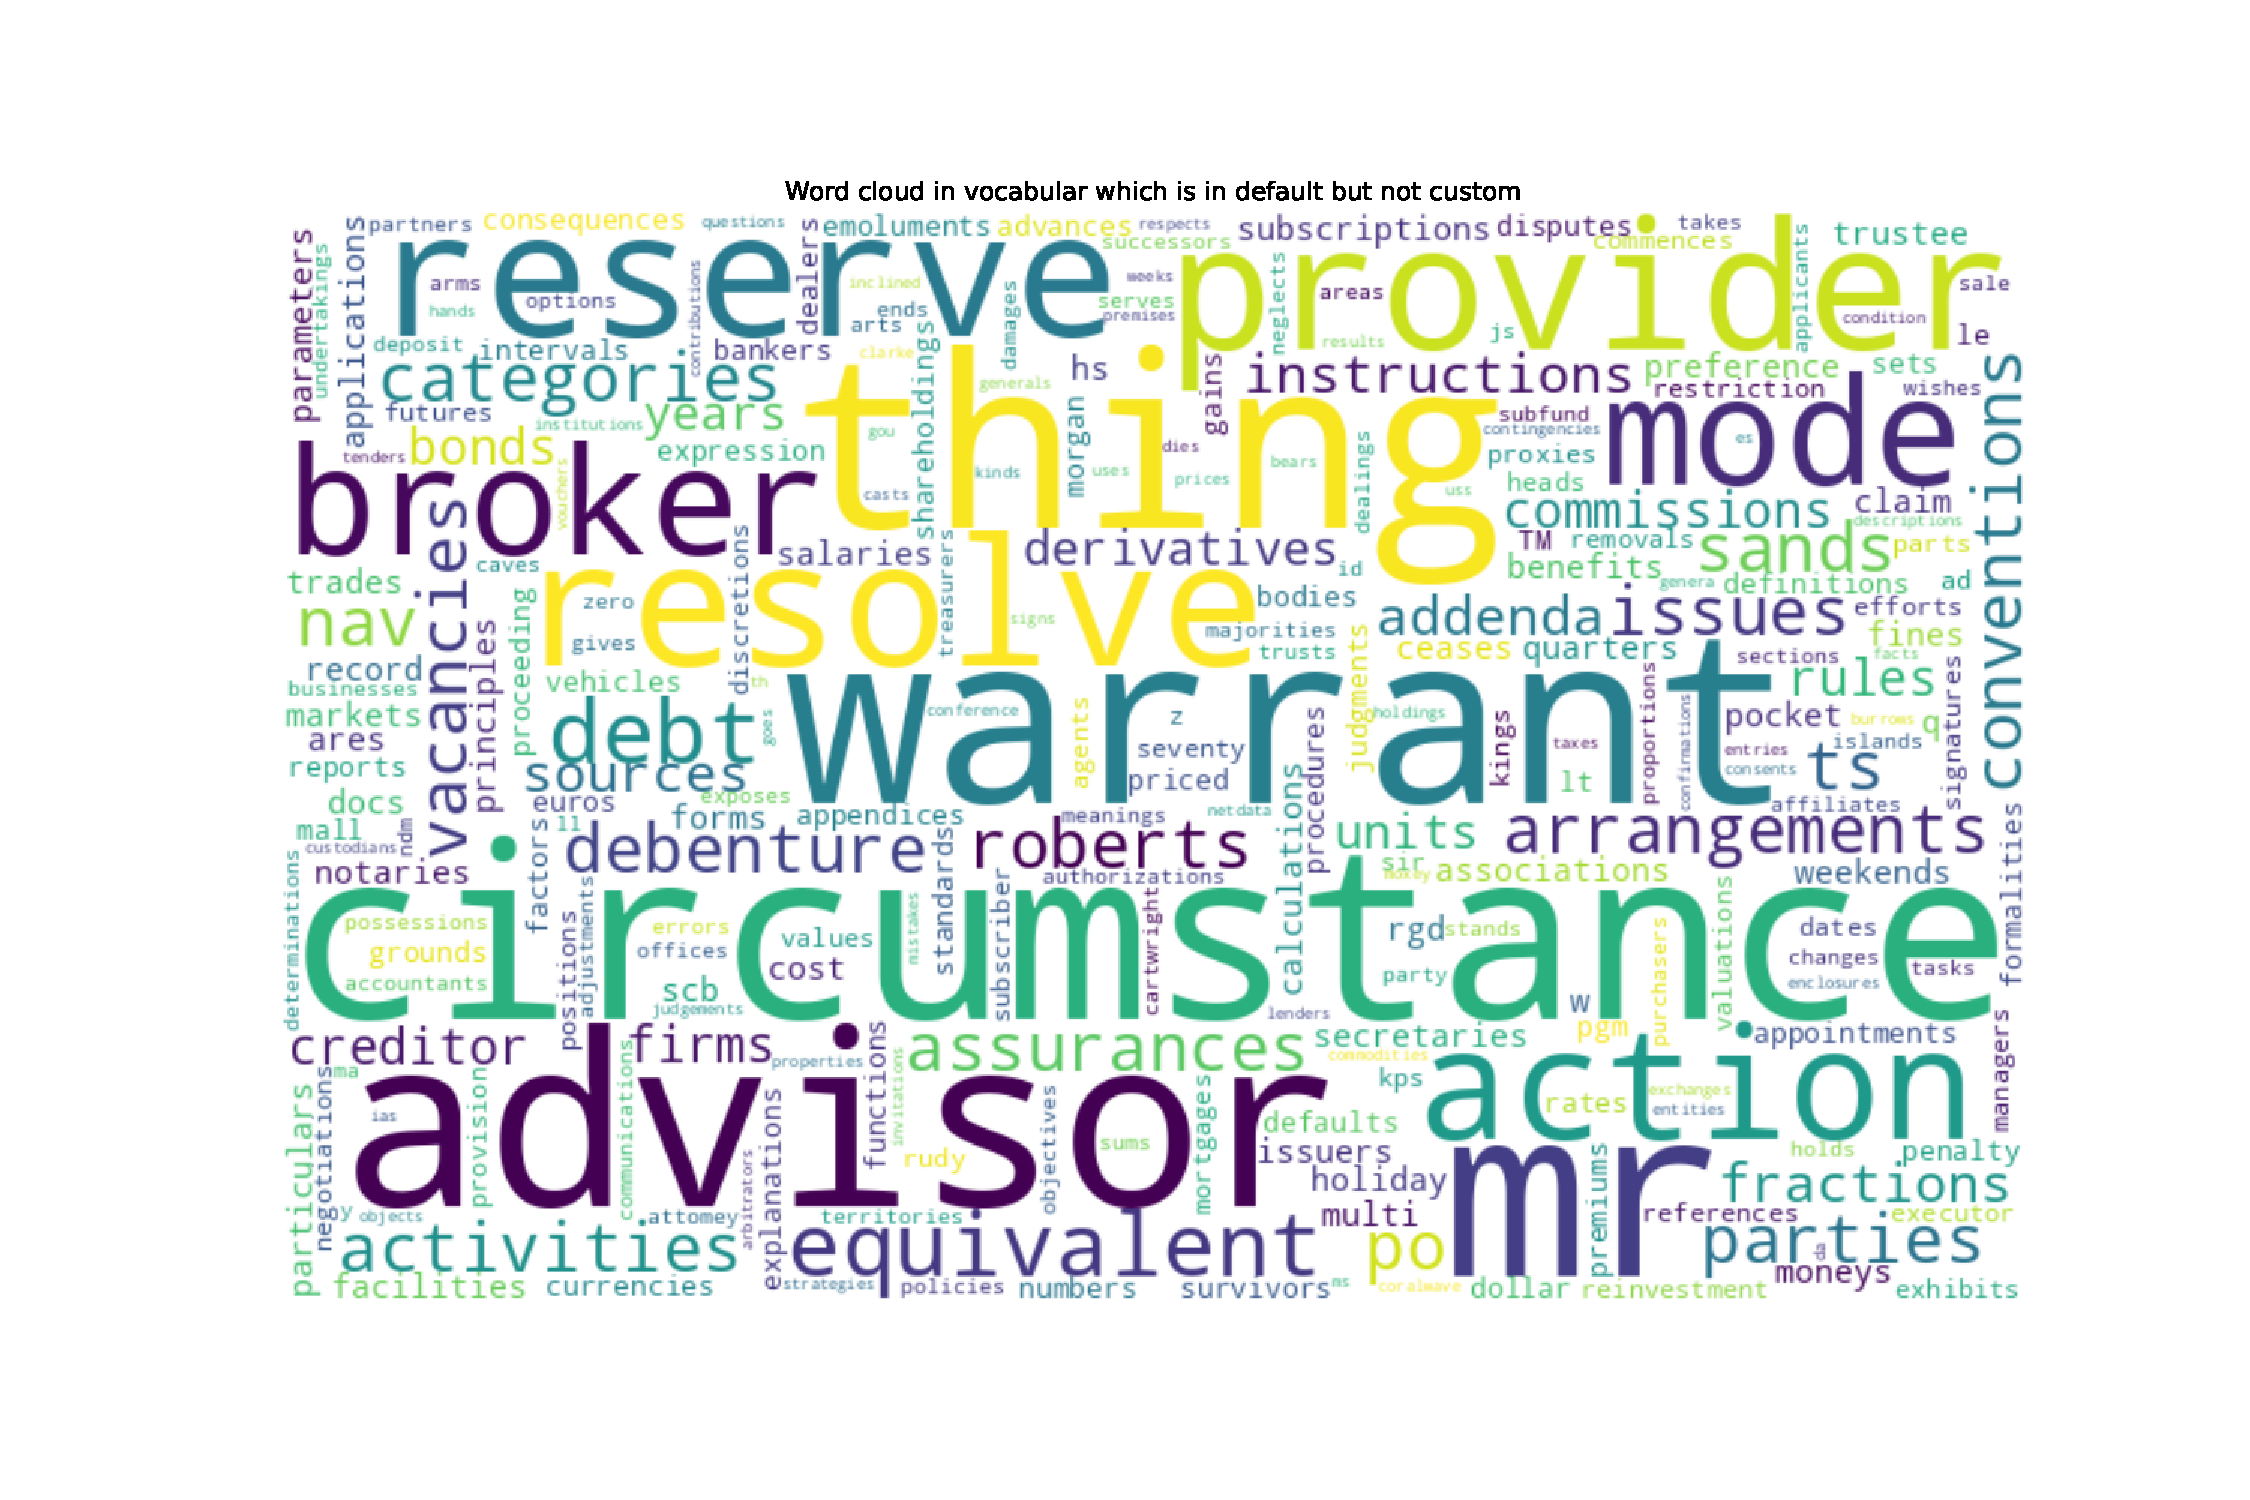
\includegraphics[width=6.8cm]{images/embeddings/tfidf/Word_cloud_in_vocabular_which_is_in_default_but_not_custom.pdf} }}%
    \qquad
    \subfloat[\centering The terms only present in the vocabulary obtained from the custom preprocessor.]{{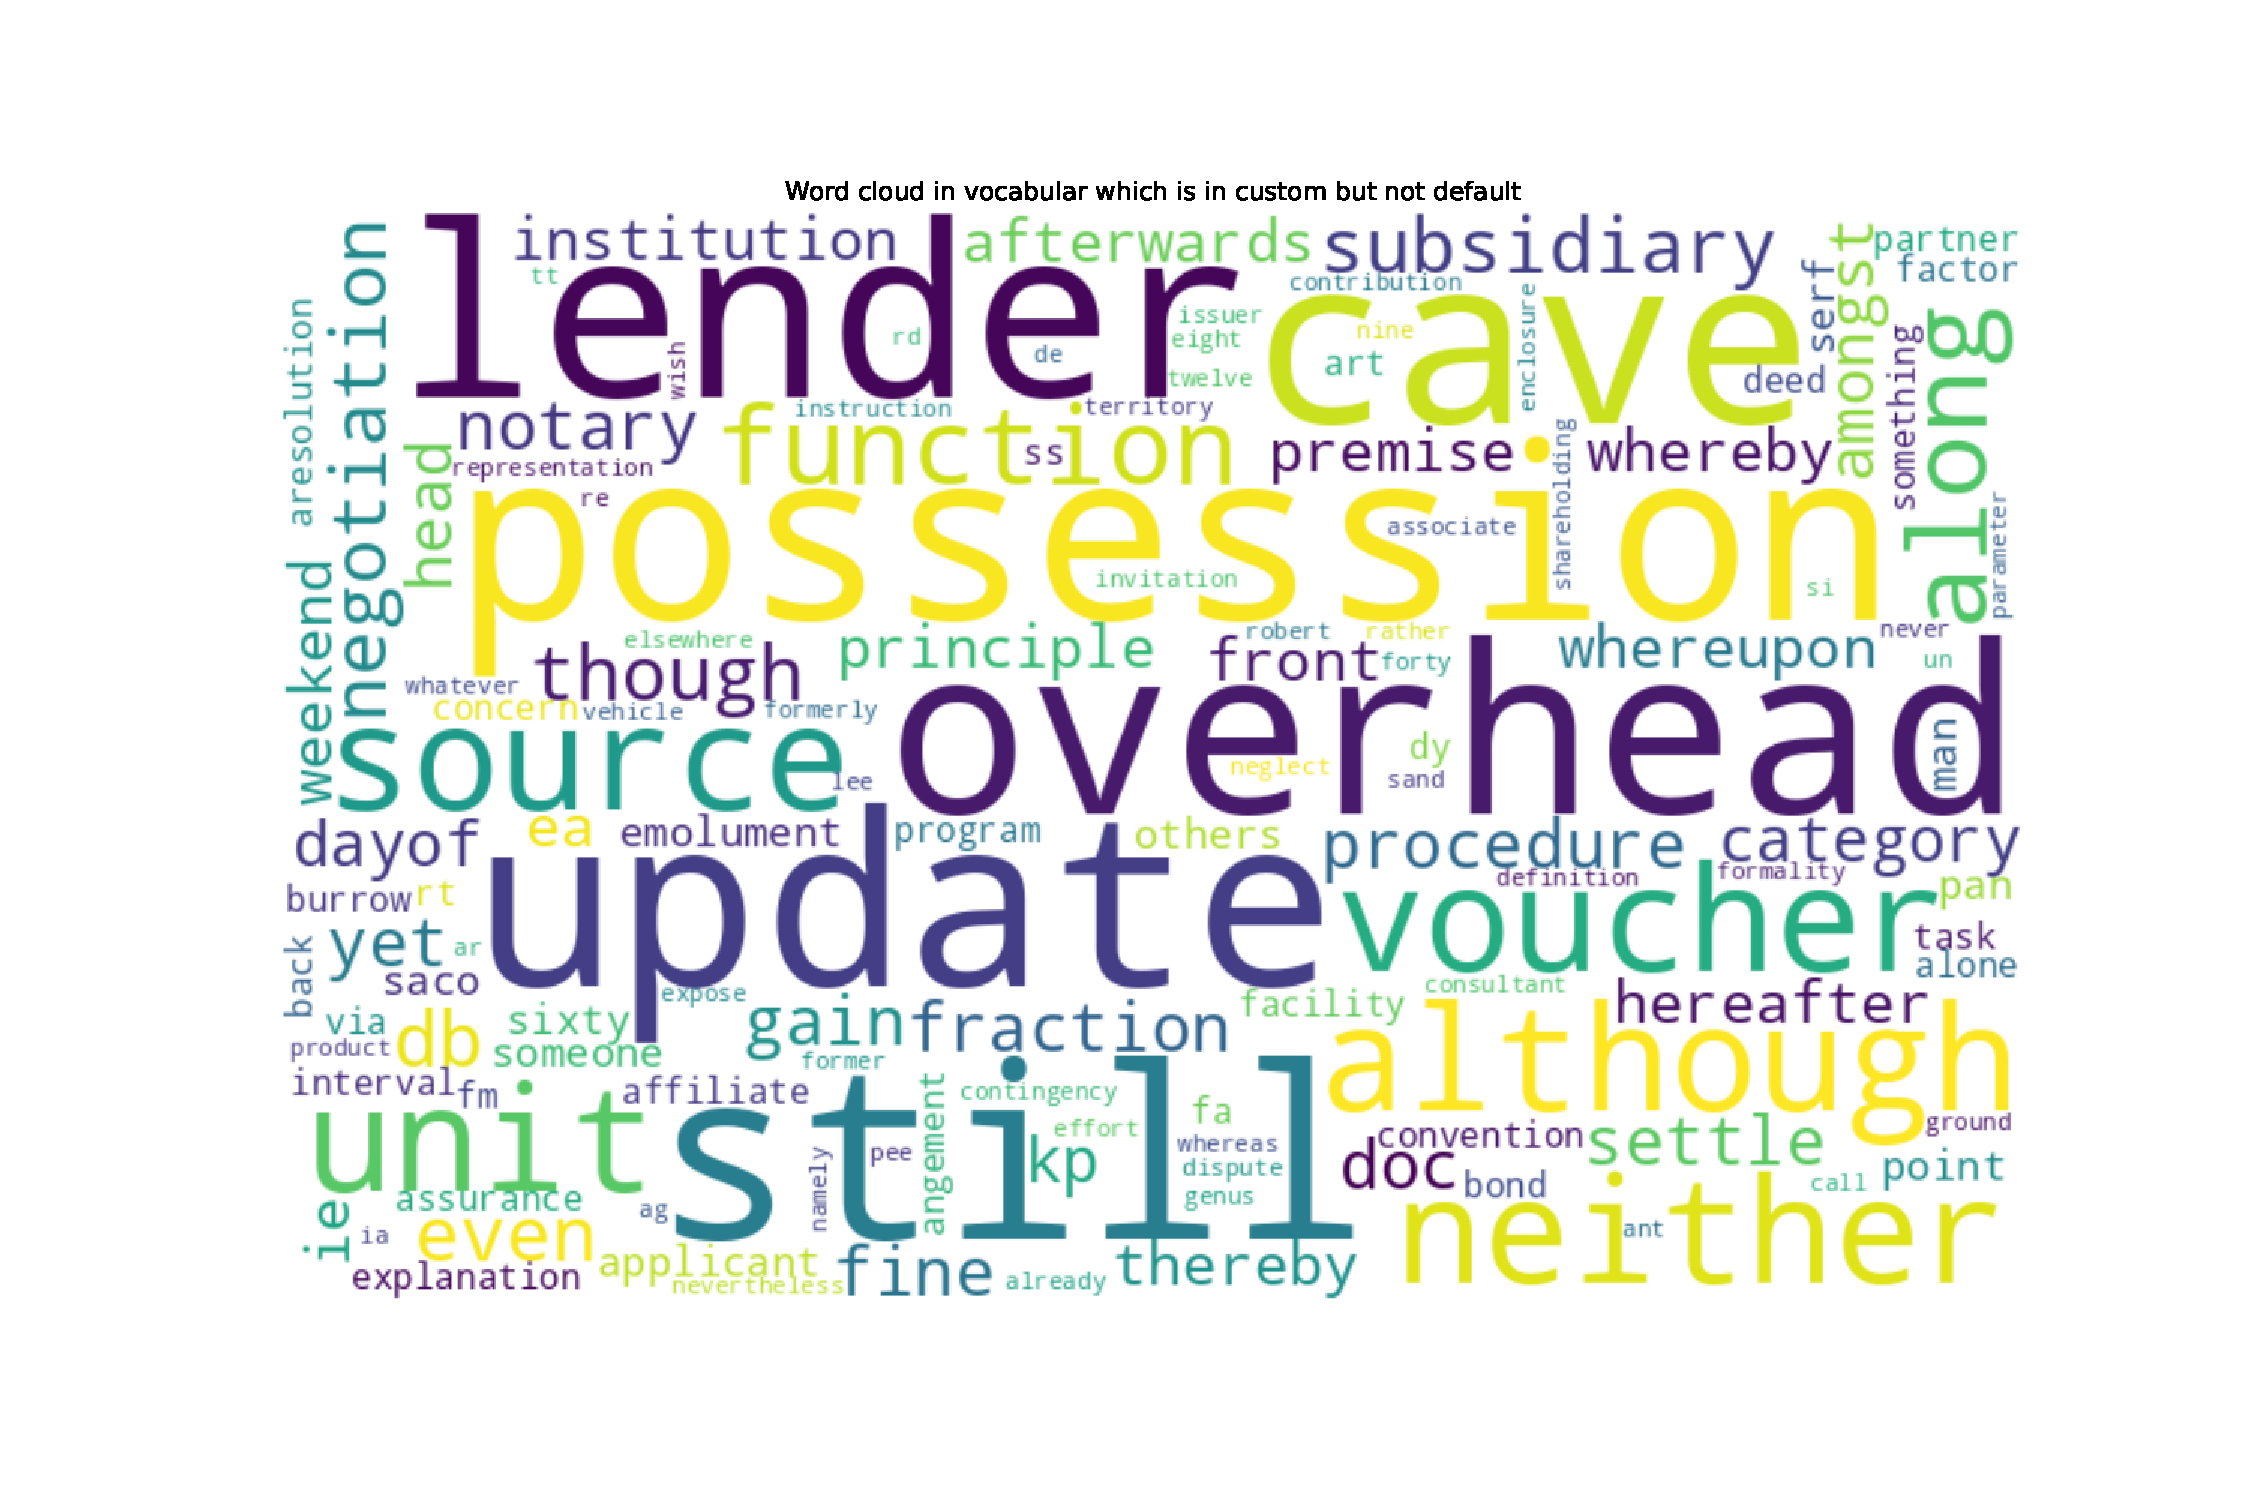
\includegraphics[width=6.8cm]{images/embeddings/tfidf/Word_cloud_in_vocabular_which_is_in_custom_but_not_default.pdf} }}%
    \caption[\wordcloud{}s for different \ac{tfidf} preprocessors]{The \wordcloud{}s visualize which words are unique to both vocabularies 
    on a random selection of 2048 documents.}%
    \label{fig:differences-vocabularies}%
\end{figure}

% two fields in db
Initially, there should have been two different \ac{tfidf} models.
The first one should have been used to obtain documents which are similar to the query document.
Therefore, terms that occur only once in the corpus should have been removed from the vocabulary.
The second approach should have been used to obtain specific documents from the corpus.
Hence, the vocabulary should consist of very document-specific terms and thus, \texttt{max\_df} would have been relatively low, to omit terms that occur in many documents.
However, the restrictions imposed by the database implementation in terms of dimensionality limitations
made it impossible to explore many parameter ranges.
Therefore, only one \ac{tfidf} model is used in the end, whose parameters \texttt{min\_df} and \texttt{max\_df} are set to values 
which kept the vocabulary size small and thus,
the dimensionality of the embeddings is reasonably small.

\subsection*{\ac{d2v}}\label{subsec:evaluation-doc2vec}

Since no labeled data is available, the evaluation of the \ac{d2v} embeddings is limited.
Therefore, the \ac{d2v} embeddings are evaluated by comparing them to other embeddings.
The \ac{d2v} model is not tuned in terms of hyperparameter selection,
but the default settings are used since there is no way to evaluate the resulting embeddings.


\subsection*{\infersent{}}\label{subsec:evaluation-inferSent}

% pool type
The \texttt{max} pooling type is used for the \infersent{} model, since \citeauthor{inferSent2018} 
found by conducting experiments using different pooling techniques that it was the best option.

% version/ embeddings dictionary
Initially, in this work, the \ac{glove} word embeddings were used for the \infersent{} model.
However, since the file of precomputed \acs{glove} word embeddings has a size of 5.65 \ac{gb} and thus,
slows down the model, ultimately another word embedding was used.
The time necessary to compute and insert 195 documents for specific embeddings is displayed in \autoref{fig:times_emb}.
The custom word embedding used in this work is a \ac{w2v} model trained on a selection of 195 documents from the Bahamas dataset.

% glove
\citeauthor{glove2014} state that \acs{glove} outperforms \ac{w2v} on the same corpus, 
vocabulary and window size in terms of quality and speed \cite{glove2014}.
Hence, the quality of the results obtained in this work may have suffered from using a custom \ac{w2v} instead of \acs{glove}.
However, since the computation time of the project is a crucial factor, the custom \ac{w2v} was used.

\begin{figure}%
    \centering
    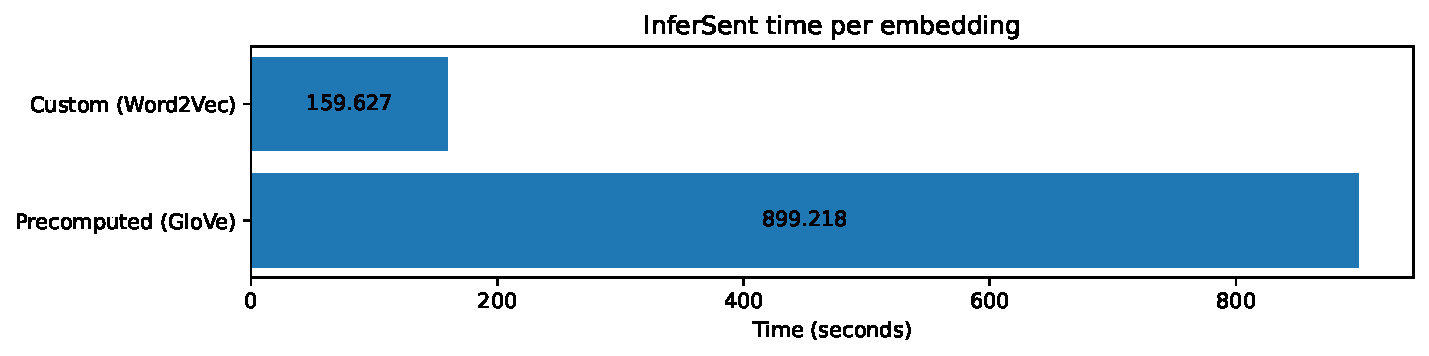
\includegraphics[width=0.6\textwidth]{images/embeddings/infersent/InferSent_time_per_embedding.pdf}
    \caption[Times for \infersent{} embeddings per precomputed word embedding]
    {Time necessary to calculate and insert \infersent{} embeddings for different precomputed word embeddings on a \localMaschineStats{}.
    }
    \label{fig:times_emb}%
\end{figure}


\section{Evaluation of \ac{use}}\label{sec:evaluation-use}

Since there are no parameters to customize the evaluation of the \ac{use} embeddings is limited.
Therefore, the \ac{use} embeddings are evaluated by comparing them to other embeddings.

\subsection*{\ac{ae}}\label{subsec:evaluation-ae}

% architecture
In order to determine, which architecture for the hidden or so-called latent space of the \ac{ae} is the best option, 
different architectures were tested and compared in terms of \ac{rsme} and cosine similarity.
The \ac{rsme} is calculated as given in \lst{lst:impl-rsme}.
The cosine similarity is calculated as given in \lst{lst:impl-cos_sim}.
Due to the fact that cosine similarity values are bound by 0 and 1, they are easier to rank than metrics that can yield any real number.
However, cosine similarity is usually applied to calculate the angle between two vectors and thus, one has to be cautious when interpreting the result obtained.
For instance, the vectors $\left( 0, 1 \right)^T$ and $\left( 0, 2 \right)^T$ have a cosine similarity of 1, even though they are not the same vectors.
Since an \ac{ae} is supposed to reconstruct the input rather than return a dependent or related vector, this metric should be combined with a tarditional metric.
The dataset used for the evaluation is a selection of 195 documents from the Bahamas dataset.

% RSME
\begin{listing}[htp]
    \begin{minted}{python3}
        rsme = np.linalg.norm(inverse_embedding - embeddings) 
                / np.sqrt(embeddings.shape[0])
    \end{minted}
    \caption[Computation of the \ac{rsme}]{
        Computation of the \ac{rsme} between the original and the reconstructed embedding.
    }
    \label{lst:impl-rsme}
\end{listing}

% cosine similarity
\begin{listing}[htp]
    \begin{minted}{python3}
        cos_sim = statistics.mean([np.dot(inverse_emb, embedding)
                /(np.linalg.norm(inverse_emb)*np.linalg.norm(embedding)) 
                for inverse_emb, embedding in zip(inverse_embedding, embeddings)])
    \end{minted}
    \caption[Computation of the cosine similarity]{
        Computation of the cosine similarity between the original and the reconstructed embedding.
    }
    \label{lst:impl-cos_sim}
\end{listing}

The scores of different architectures are shown in \fig{fig:eval-ae-architecture}.
While most of the architectures produced similar results, one architecture stood out.
Combining 2500-, 3000- and 3500-dimensional layers in the hidden space produced the worst \ac{rsme} results.
The best results were achieved by adding a 3500-dimensional layer in the hidden space.
However, the results of the best architecture do not differ greatly from the others.

\begin{figure}[!htb] % htp = hier (h), top (t), oder auf einer eigenen Seite (p).
    \centering
    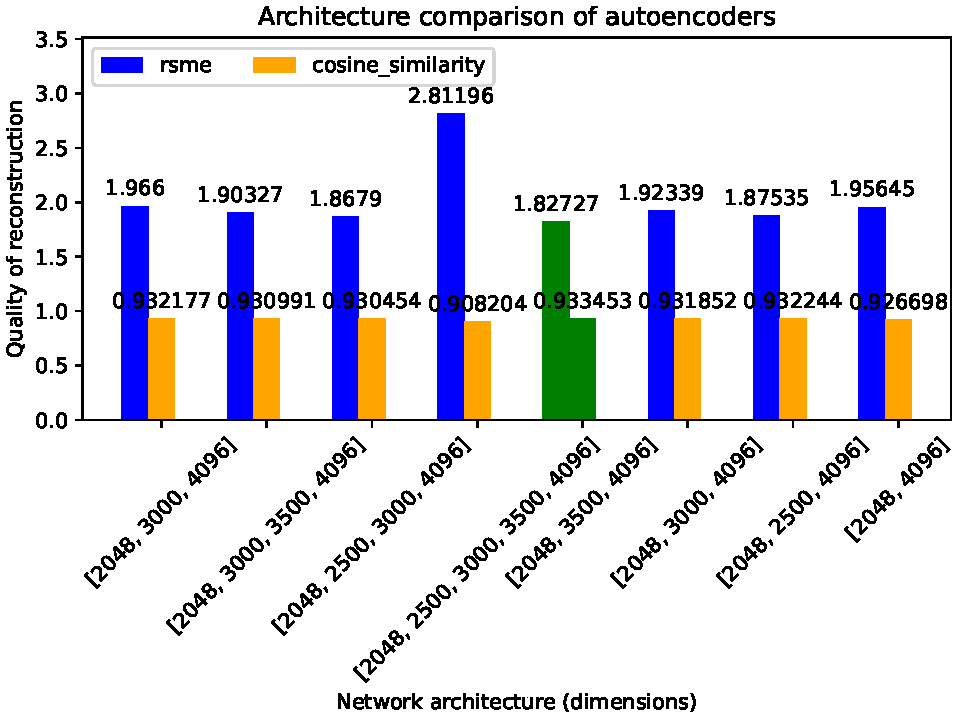
\includegraphics[width=1\textwidth]{images/embeddings/autoencoder/ae_score_plot.pdf}
    \caption[Different \ac{ae} architectures and their reconstruction error]{The effect of different \ac{ae} architectures on the reconstruction error.
    The error is measured in terms of \ac{rsme} (blue bars) and cosine similarity (yellow bars) between the original and the reconstructed image.
    The smallest \ac{rsme} and the biggest cosine similarity belong to the architecture best suited to this task and are coloured green.
    }
    \label{fig:eval-ae-architecture}
\end{figure}

% Clustering
\section{Clustering using \acs{optics}}\label{sec:evaluation-OPTICS}
% 3d plots
The algorithm \ac{optics} was applied to data, which was preprocessed according to \autoref{pt:32} and \autoref{pt:eigendocs}.
The clusters from \autoref{fig:optics_cluster} were extracted from the respective reachability plots in \autoref{fig:reachability_plots}.
The three-dimensional plots visualize the first three dimensions of the data and thus, the weights of the first three principal components assigned by the \eigendocs{} algorithm.
By visual inspection and comparison of both plots, it can be seen that the projection by the combination of resizing and \ac{pca} of \autoref{pt:32} scatters the objects further along the $x_2$ axis.
Hence, the distance between the objects is larger and more clusters are identified.
One could argue that the narrow distribution of the objects in the \eigendocs{} plot is due to the fact, 
that the input data encodes not only the visual appearance in terms of page layout but also the size of the document.
Possibly, this could explain why the objects are less scattered along this dimension.

% OPTIC cluster results
\begin{figure}%
    \centering
    \subfloat[\centering Preprocessing according to \autoref{pt:32}.]{{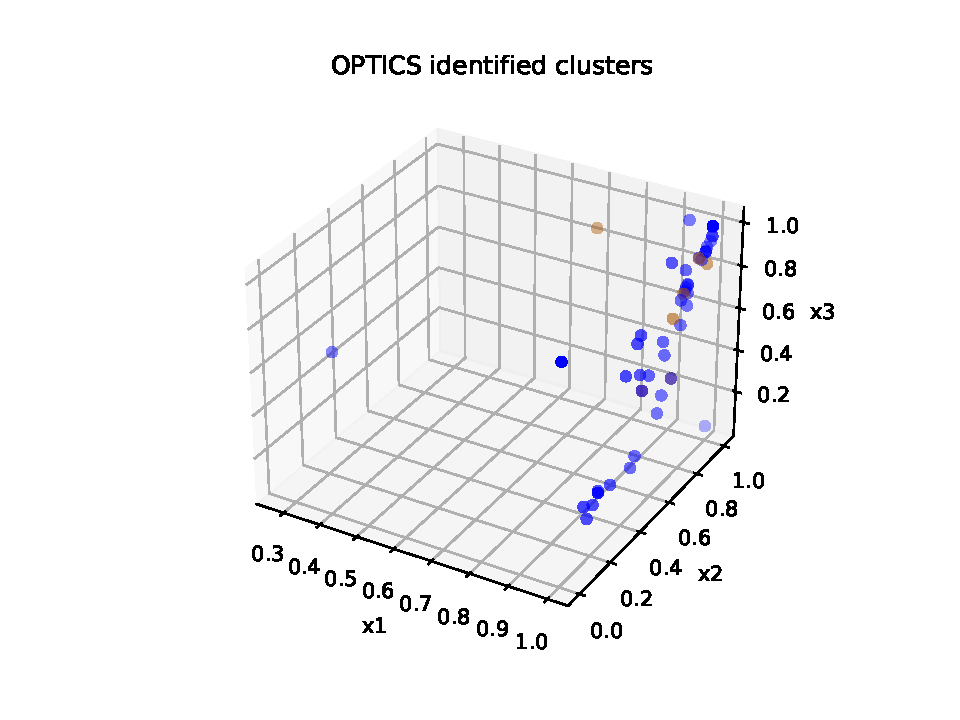
\includegraphics[width=5cm]{images/OPTICS/32x32/OPTICS_cluster_32x32.pdf} }}%
    \qquad
    \subfloat[\centering Preprocessing according to \autoref{pt:eigendocs}.]{{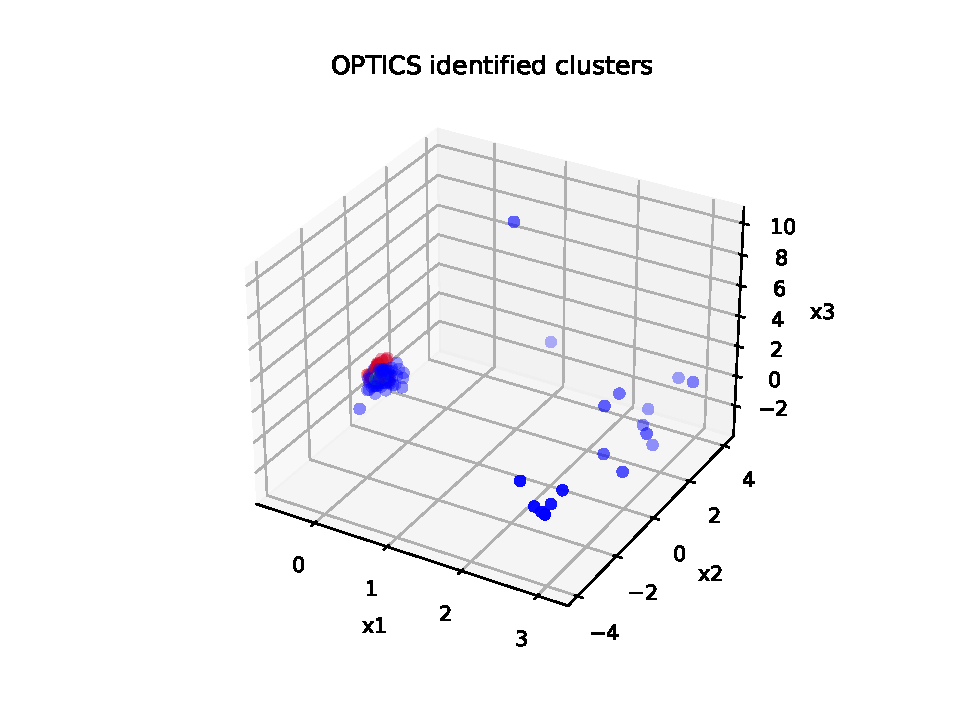
\includegraphics[width=5cm]{images/OPTICS/eigendocs/OPTICS_cluster_eigendocs.pdf} }}%
    \caption[\ac{optics} clusters]{The clusters were extracted from the respective reachability plots in \autoref{fig:reachability_plots} by \ac{optics}.
    The blue points are noise points, whereas any other colour denotes a cluster.}%
    \label{fig:optics_cluster}%
\end{figure}



% cluster content
To analyse the results of the clustering, the content of the clusters was examined.
Since the documents are not labelled, the content of the clusters was analysed by visual inspection.
The content of the clusters is displayed in \autoref{fig:clusters_32x32} and \autoref{fig:clusters_eigendocs_with_noise}.
The yellow images belong to the group identified as noise.
The images preprocessed according to \autoref{pt:32} were partitioned into multiple small and one big cluster.
The \eigendocs{} images' clusters have similar sizes. 
The row of noise images is thus, way longer than the other rows in \autoref{fig:clusters_eigendocs_with_noise}.
Most of the certificates are classified as noise for both approaches.


% 32x32
\begin{figure}[htp] % htp = hier (h), top (t), oder auf einer eigenen Seite (p).
    \centering
    \includegraphics[width=1.05\textwidth]{images/OPTICS/32x32/cluster_content_32x32.pdf}
    \caption[Detailed \ac{optics} clusters using 32x32 greyscale pixels]{The yellow images belong to the group denoted noise.
    Most certificates are classified as noise.
    There is one big cluster and multiple small clusters.
    The images were preprocessed as discussed in \autoref{pt:32} to 32x32 greyscale pixels.
    }
    \label{fig:clusters_32x32}
\end{figure}

% eigendocs with noise
\begin{figure}[htp] % htp = hier (h), top (t), oder auf einer eigenen Seite (p).
    \centering
    \includegraphics[width=1.05\textwidth]{images/OPTICS/eigendocs/cluster_content_incl_noise_Eigendocs.pdf}
    \caption[Detailed \ac{optics} clusters using \eigendocs{}]{Most certificates are classified as noise. The rest of the clusters have similar sizes.
    The images were preprocessed as discussed in \autoref{pt:eigendocs} to 13-dimensional greyscale pixels.
    }
    \label{fig:clusters_eigendocs_with_noise}
\end{figure}


The preprocessing approach used to create the \ac{optics} input for the \databaseName{} database index is \eigendocs{} since it also encodes information about the document size. 

% code
According to \citeauthor{OPTICS2014}, \ac{optics} was developed to improve \ac{dbscan} flaws.
Therefore, \ac{dbscan} is chosen for the cluster method in \lst{lst:optics_model}, since the literature consulted works with \ac{dbscan} as a basis.
In order to reduce calculation complexity the maximum $\varepsilon$ is 10.
The distance between two points to still be considered neighbours is defined after visual inspection of the reachability plot.
Considering the intrinsic structure of the data it is set to $0.5$ to return meaningful clusters.

% Eval models and baseline
\section{Comparison of models}\label{sec:evaluation-models}

% parameters
Similar to \citeauthor{glove2014}'s work, in this work, for many models used, any unspecified parameters are set to their default values, 
assuming that they are close to optimal
acknowledging that this simplification should be revised in a more thorough analysis.

% comparing models (qualitative)
This evaluation does not aim to find the best model but to compare the similarity of the models' query results.
The different query responses of the models are compared on a selection of documents.
The selection is obtained by randomly choosing \textcolor{red}{TODO: X} documents from a corpus of 2048 documents.
The 2048 document corpus was randomly chosen (without replacement) from the Bahamas leak.
The \textcolor{red}{TODO: Y} most similar documents for each selected document are retrieved from the database for each model and stored in a \ac{csv} file.
To facilitate working with the data, the document IDs can be encoded as monotonically increasing integers.

Furthermore, the query results are compared using a Venn diagram and a heatmap presented in \autoref{fig:comparison-models}.
% Venn diagram
To build a Venn diagram, the number of documents which are shared between the query results of two models is computed.
Hence, all query results of a model are saved in a set and the intersection of two sets is computed.
Since there are five models the Venn diagram consists of five circles.
It is possible to compare not only two but more models at once.
One should be cautious when interpreting the layout of the Venn diagram since 
an intersection of documents which produces an empty set has a non-empty area in this visualization.
\textcolor{red}{results derived from diagram}

% heatmap
Before the heatmap can be created, the shared query results of each model pair are computed and stored in a matrix.
The matrix consists of five rows and five columns, where each row and column represents a model.
The code snippet in \lst{lst:sim-matrix} shows the calculation of the similarity matrix.
The cell values are the number of shared query results between the models of the row and column.
They are calculated by summing up the number of shared query results per document query.
Since the matrix is symmetric, only the upper triangular matrix is computed and the other half is mirrored.
The matrix is then visualized using a heatmap.
\textcolor{red}{results derived from diagram}

\begin{listing}[htp]
    \begin{minted}{python3}
        sim_matr = np.matrix(np.zeros((len(model_names), len(model_names))))
        for id in df.index:
            for i, model in enumerate(model_names):
                for j in range(i, len(model_names)):
                    sim_matr[i, j] += np.sum([df.loc[id, 
                        model_names[j]].count(item) for item in df.loc[id, model]])
                    sim_matr[j, i] = sim_matr[i, j]
    \end{minted}
    \caption{Calculation of the similarity matrix used to produce the heatmap.
    }
    \label{lst:sim-matrix}
\end{listing}

\begin{figure}%
    \centering
    \subfloat[\centering Venn diagram of query results.]{{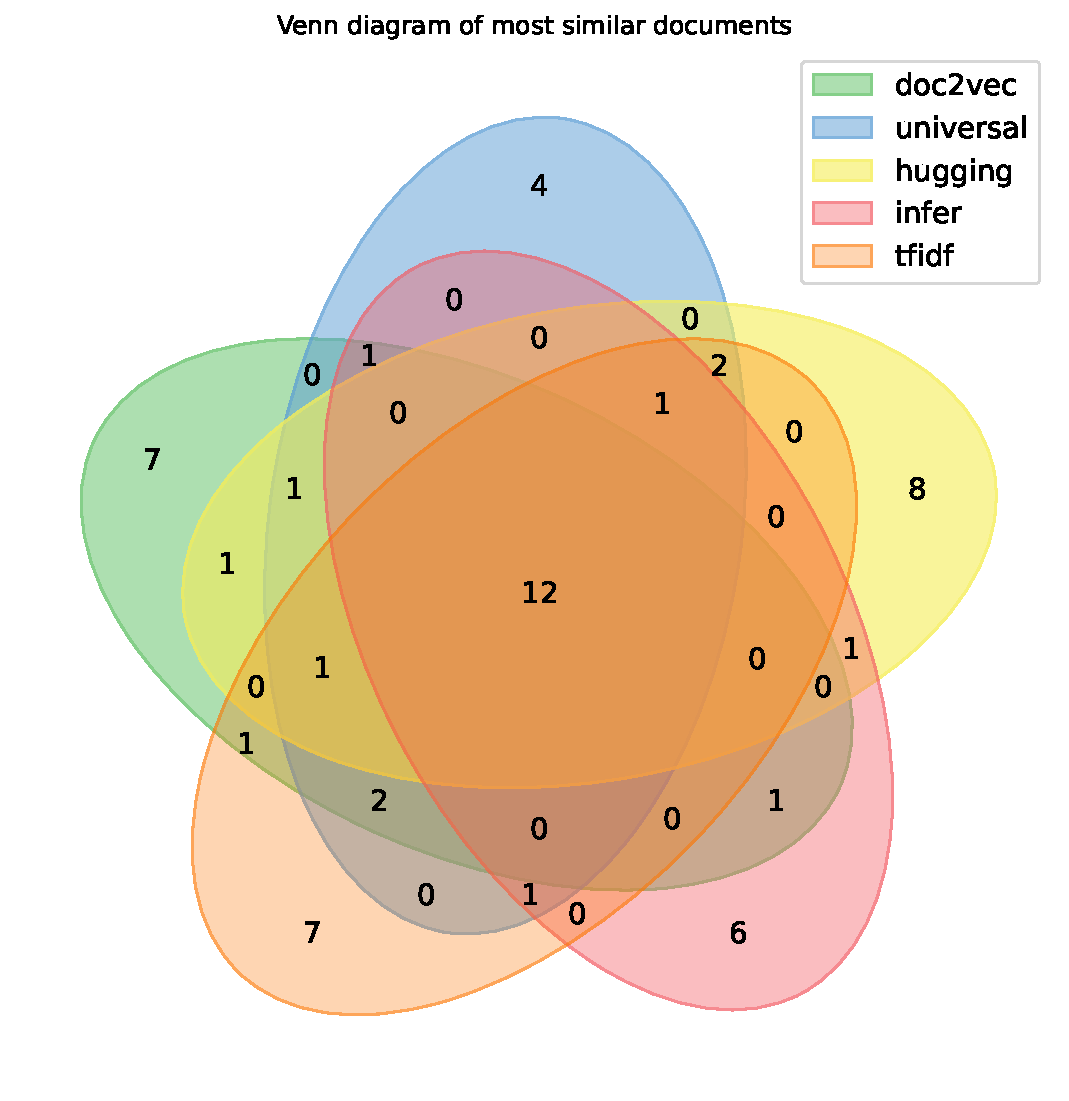
\includegraphics[width=4cm]{images/comparison/Venn_diagram_of_most_similar_documents.pdf} }}%
    \qquad
    \subfloat[\centering Heatmap visualizing shared query results.]{{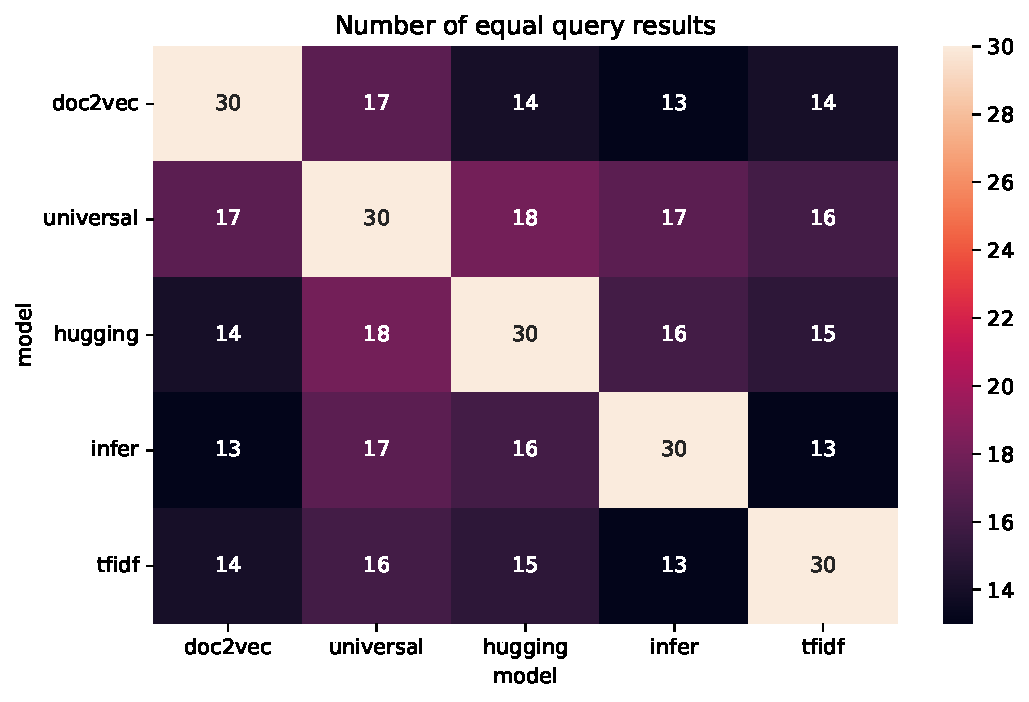
\includegraphics[width=6cm]{images/comparison/Number_of_equal_query_results.pdf} }}%
    \caption[Comparison of models]{Comparison of the results obtained by different models.}%
    \label{fig:comparison-models}%
\end{figure}


% sample query
To display the differences between the models exemplary, the five most similar documents to a random document were returned from the database and visualized.
The text of the query document was encoded using the respective model and a 
\ac{knn} query was used to obtain the results from the local database containing 2048 documents.
The query image, i.e. the one surrounded with a border, was omitted from the database query response.
The query responses are listed according to descending similarity to the query document.
\autoref{fig:query_resp_doc2vec} displays the \ac{d2v} reponses,  
\autoref{fig:query_resp_sbert} displays the \ac{sbert} reponses,  
\autoref{fig:query_resp_tfidf} displays the \ac{tfidf} reponses,  
\autoref{fig:query_resp_infer} displays the \infersent{} reponses,  
\autoref{fig:query_resp_use} displays the \ac{use} reponses.

All models except \ac{d2v} and \ac{use} returned only documents of \textit{CREDIT SUISSE}.
Apart from this difference, the query responses of the models are very similar.


% sample query
\begin{figure}[h!]
    \begin{subfigure}{\textwidth}
        \centering
        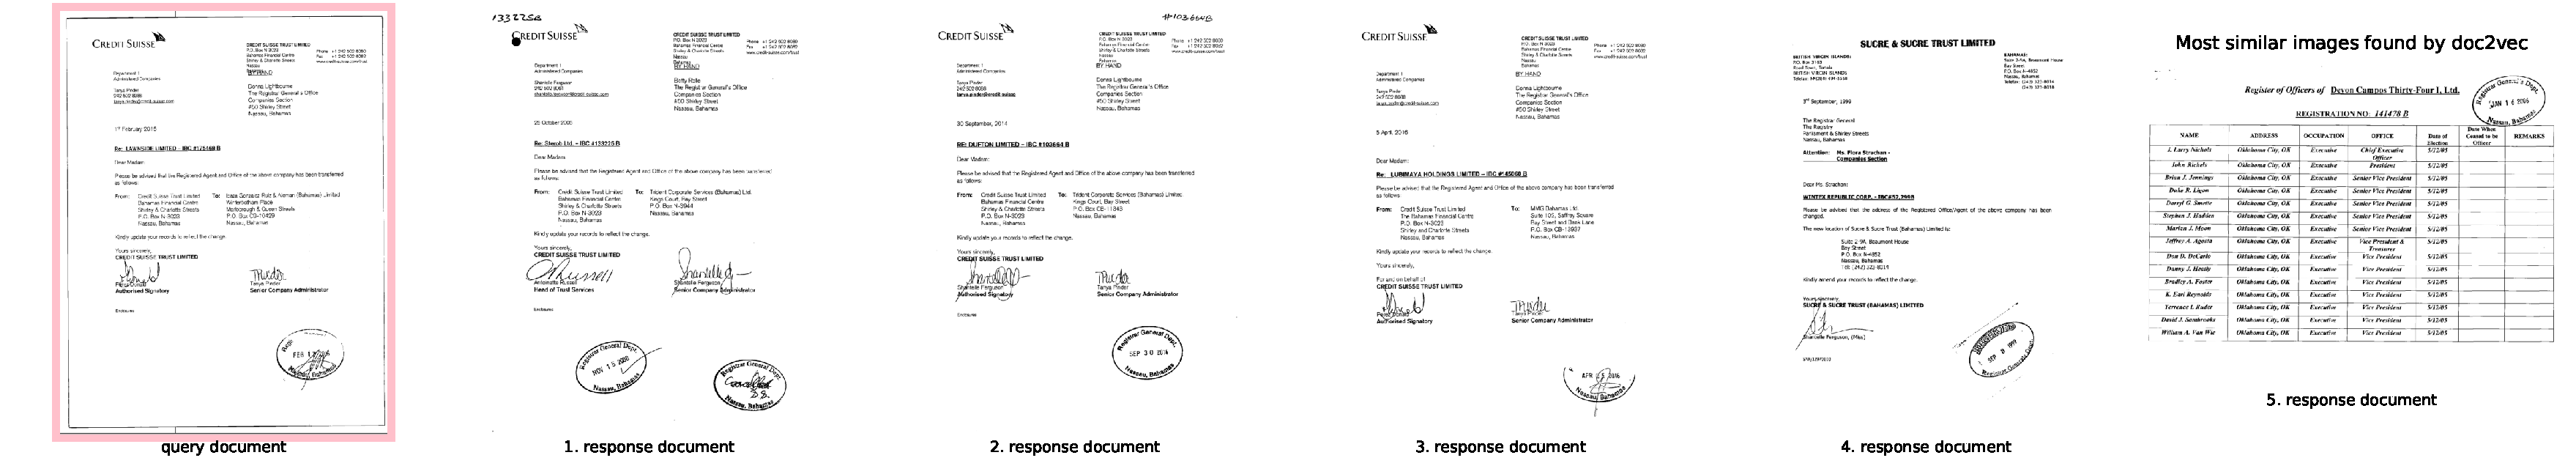
\includegraphics[width=1\textwidth]{images/query_results/4b4d0a9ee0c7283e5bfd69c402c73b2140bf90351c8f44d6809afe23c6dfaa50/Most_similar_images_found_by_doc2vec.pdf}
        \caption{\ac{d2v}}
        \label{fig:query_resp_doc2vec}
    \end{subfigure}

    \begin{subfigure}{\textwidth}
        \centering
        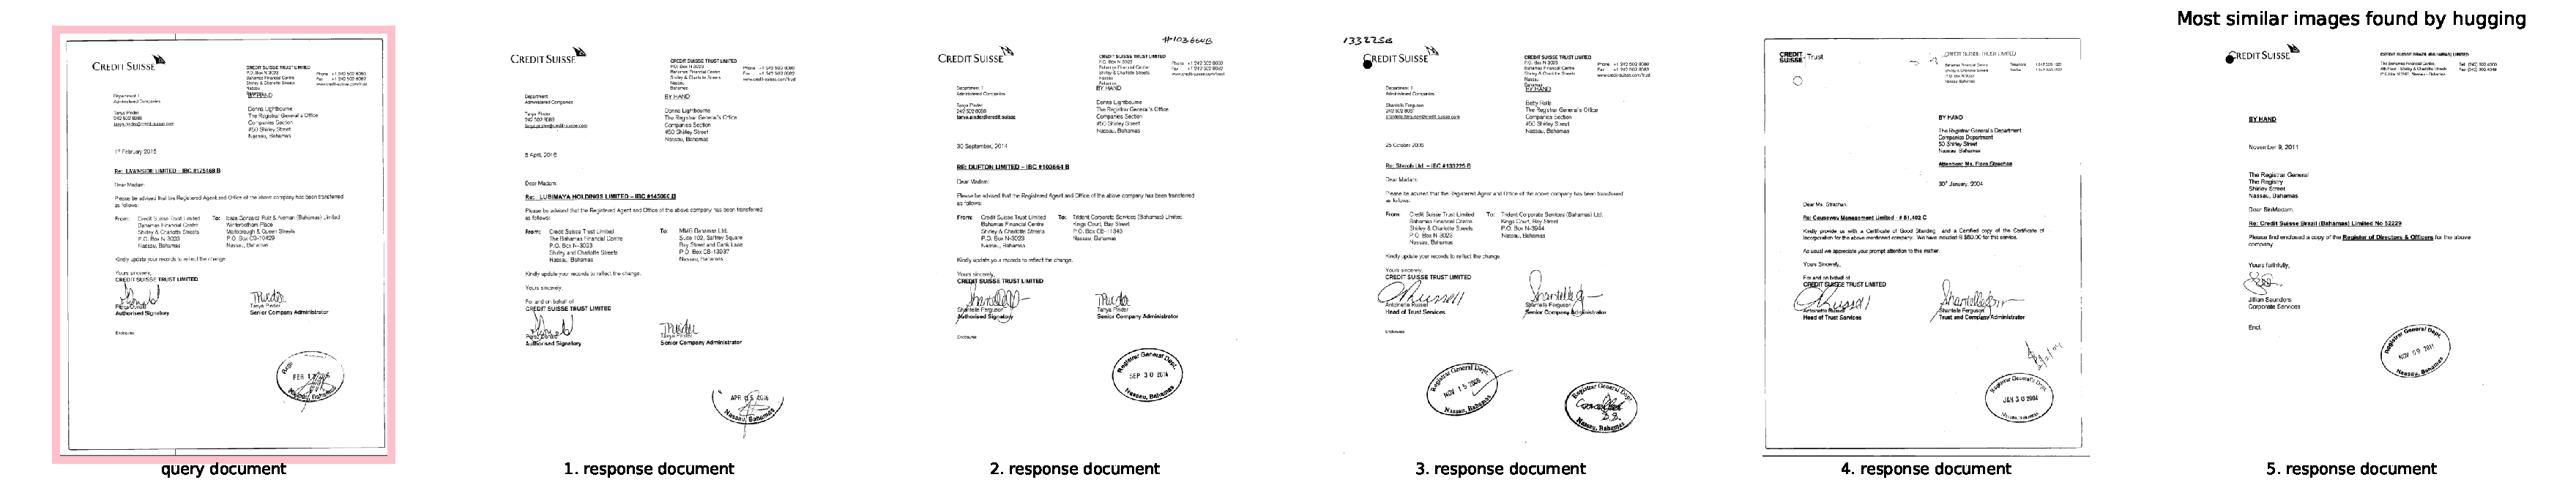
\includegraphics[width=1\textwidth]{images/query_results/4b4d0a9ee0c7283e5bfd69c402c73b2140bf90351c8f44d6809afe23c6dfaa50/Most_similar_images_found_by_hugging.pdf}
        \caption{\ac{sbert}}
        \label{fig:query_resp_sbert}
    \end{subfigure}

    \begin{subfigure}{\textwidth}
        \centering
        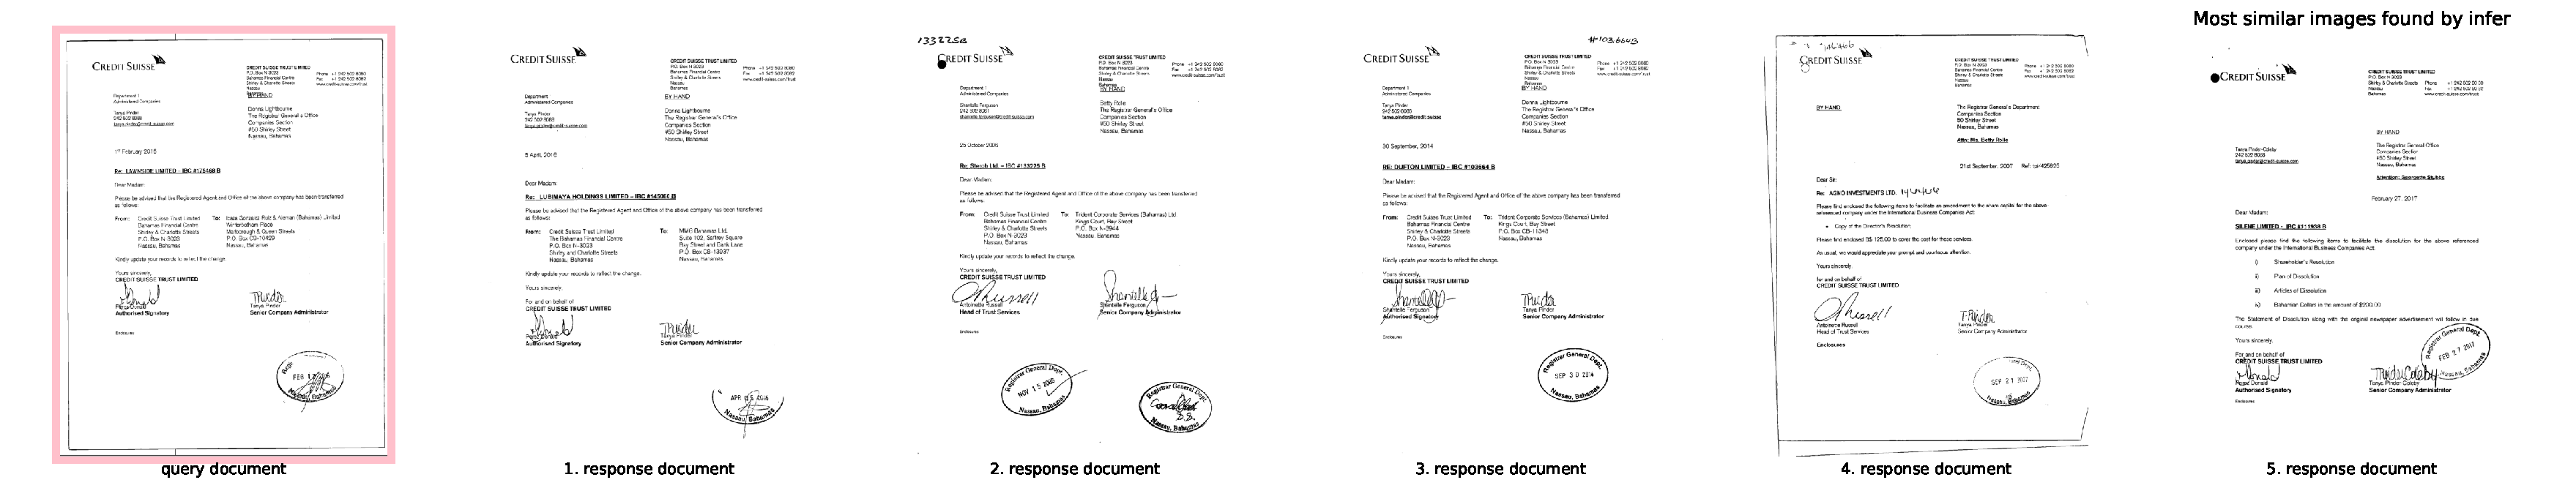
\includegraphics[width=1\textwidth]{images/query_results/4b4d0a9ee0c7283e5bfd69c402c73b2140bf90351c8f44d6809afe23c6dfaa50/Most_similar_images_found_by_infer.pdf}
        \caption{\infersent{}}
        \label{fig:query_resp_infer}
    \end{subfigure}

    \begin{subfigure}{\textwidth}
        \centering
        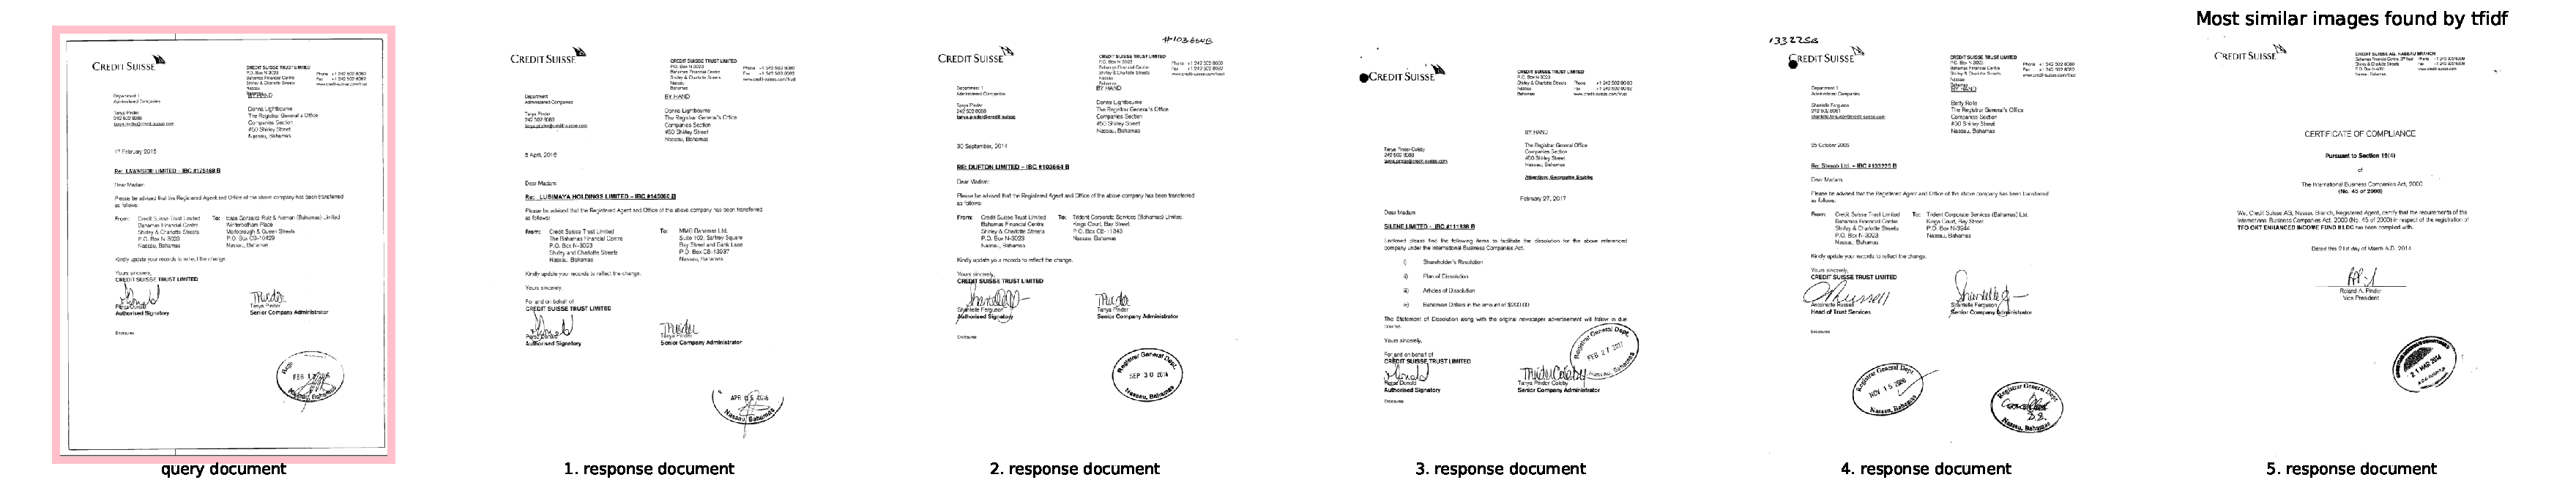
\includegraphics[width=1\textwidth]{images/query_results/4b4d0a9ee0c7283e5bfd69c402c73b2140bf90351c8f44d6809afe23c6dfaa50/Most_similar_images_found_by_tfidf.pdf}
        \caption{\ac{tfidf}}
        \label{fig:query_resp_tfidf}
    \end{subfigure}

    \begin{subfigure}{\textwidth}
        \centering
        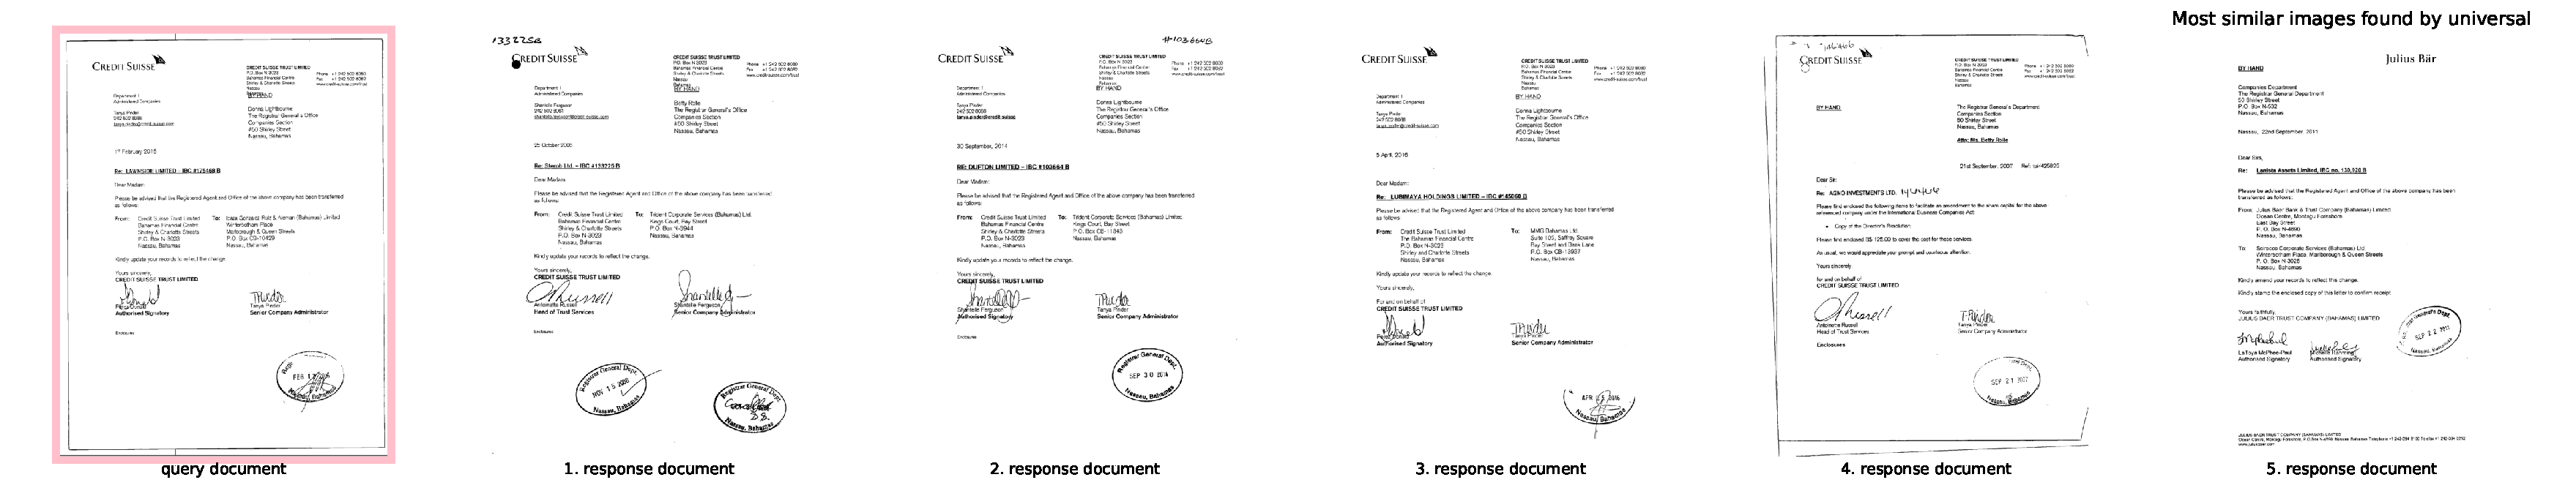
\includegraphics[width=1\textwidth]{images/query_results/4b4d0a9ee0c7283e5bfd69c402c73b2140bf90351c8f44d6809afe23c6dfaa50/Most_similar_images_found_by_universal.pdf}
        \caption{\ac{use}}
        \label{fig:query_resp_use}
    \end{subfigure}
\caption[Exemplary query response]{Response of exemplary query in terms of similarity on different embeddings.}
\label{fig:query_resp}
\end{figure}

% good results
The models produced good query responses on a query document consisting of little text.
A sample query document is shown in \autoref{fig:good_query_resp_infer}.
Even though at first glimpse, the response documents seem to appear unrelated to the query document, they share multiple words, such as \textit{director}.
Similar response documents do not have to of similar visual appreance results from the fact that the text embeddings only consider information from the text layer.

\begin{figure}[htp] % htp = hier (h), top (t), oder auf einer eigenen Seite (p).
    \centering
    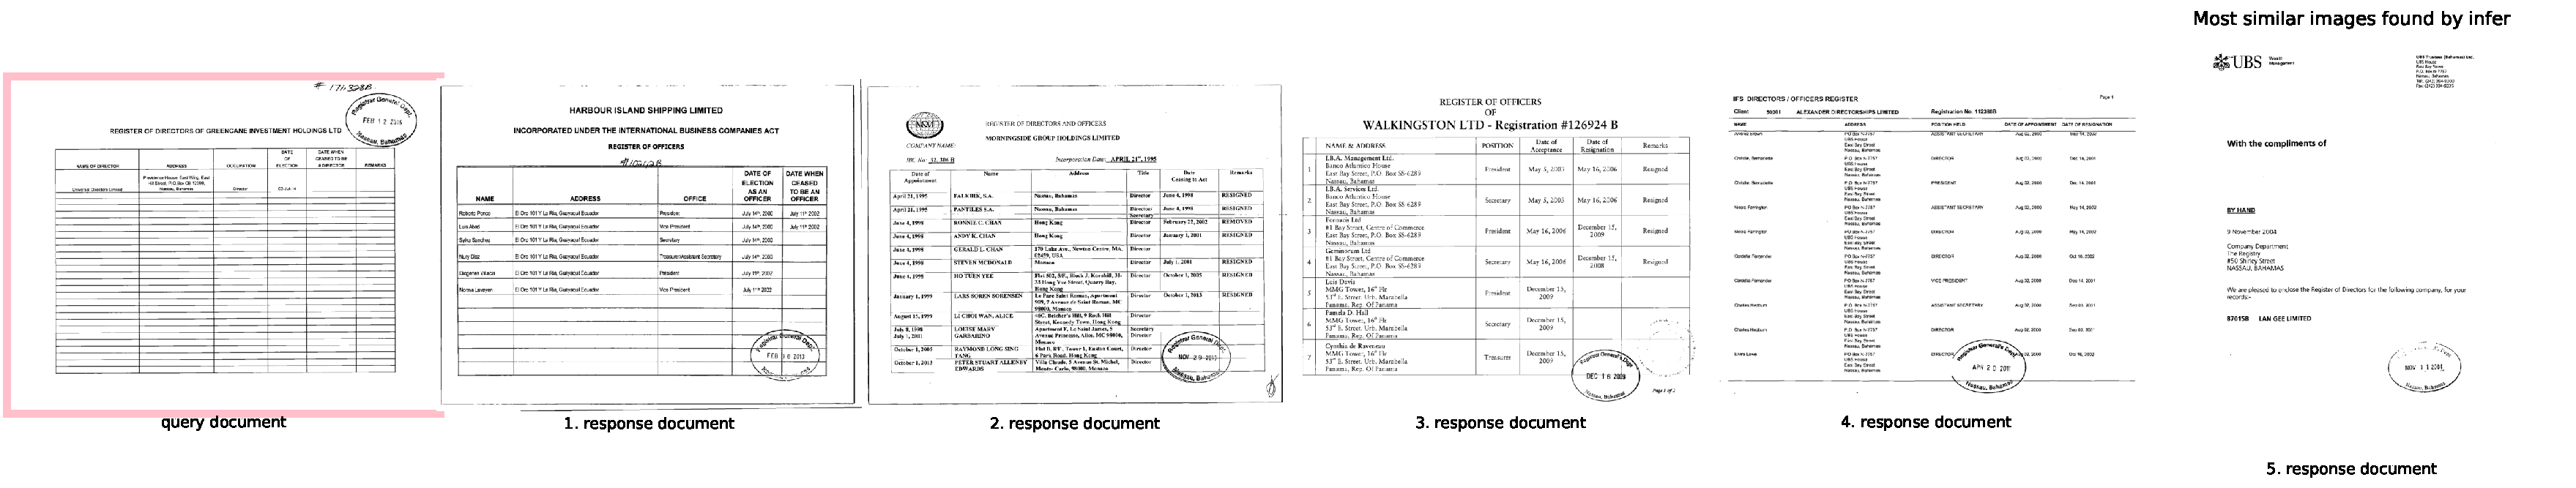
\includegraphics[width=1\textwidth]{images/query_results/42b7e56855c88c22ed01f381167e6f0887815e1ef7ea6b149be06ee1f8557b9e/Most_similar_images_found_by_infer.pdf}
    \caption[\infersent{} query responses]{\infersent{} query responses on a query document consisting of little text.
    }
    \label{fig:good_query_resp_infer}
\end{figure}

% bad results
\textcolor{red}{TODO}
\begin{figure}[h!]
    \ContinuedFloat
    \begin{subfigure}{\textwidth}
        \centering
        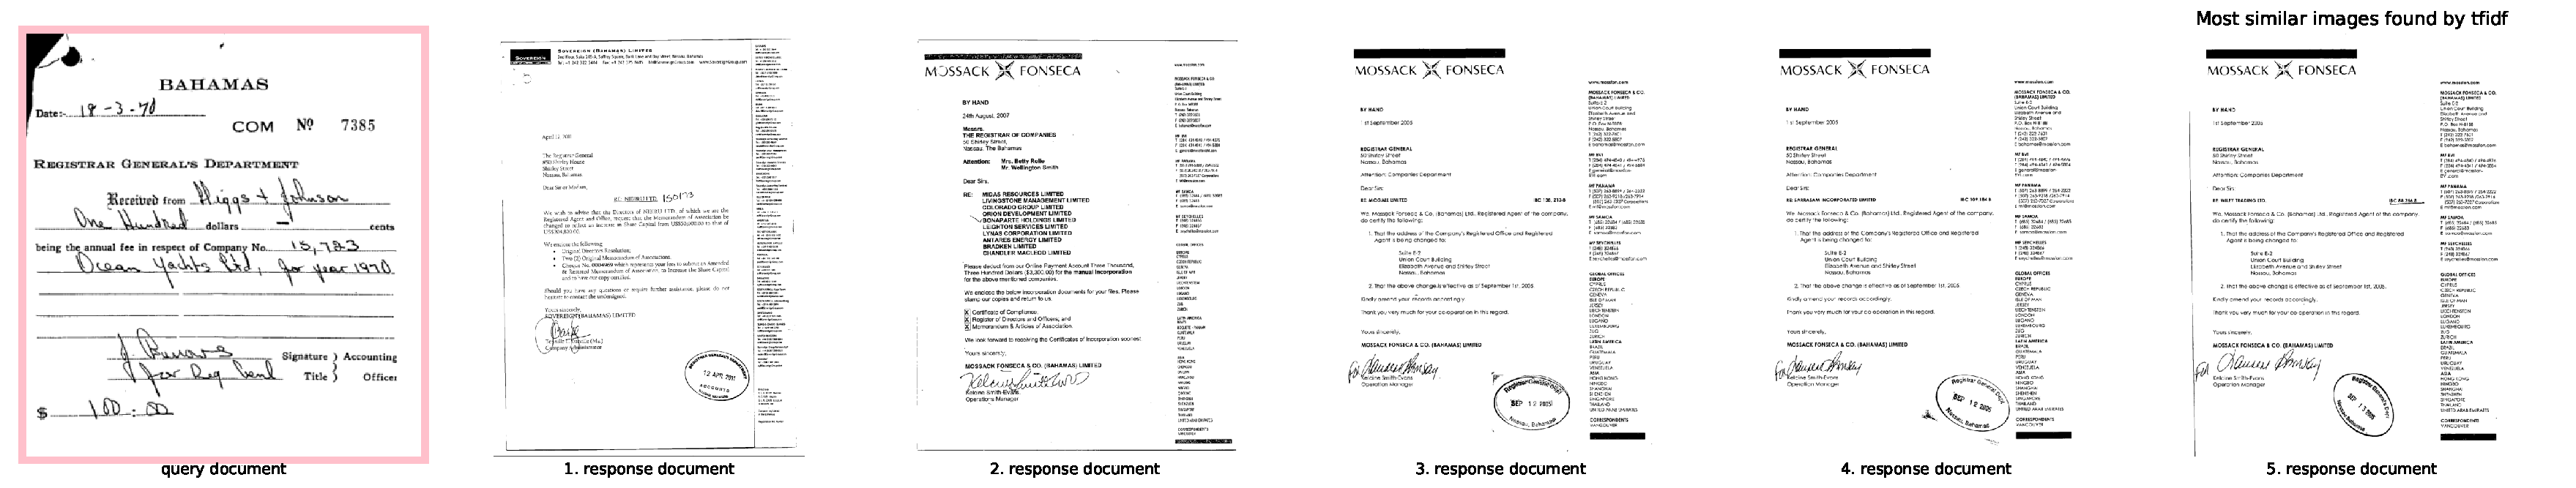
\includegraphics[width=1\textwidth]{images/query_results/4542b223317eba23e4bda3e1536d61c8e2d2890a6439830ca8c62650bc1aac70/Most_similar_images_found_by_tfidf.pdf}
        \caption{\ac{tfidf}}
        \label{fig:bas_query_resp_tfidf}
    \end{subfigure}

    \begin{subfigure}{\textwidth}
        \centering
        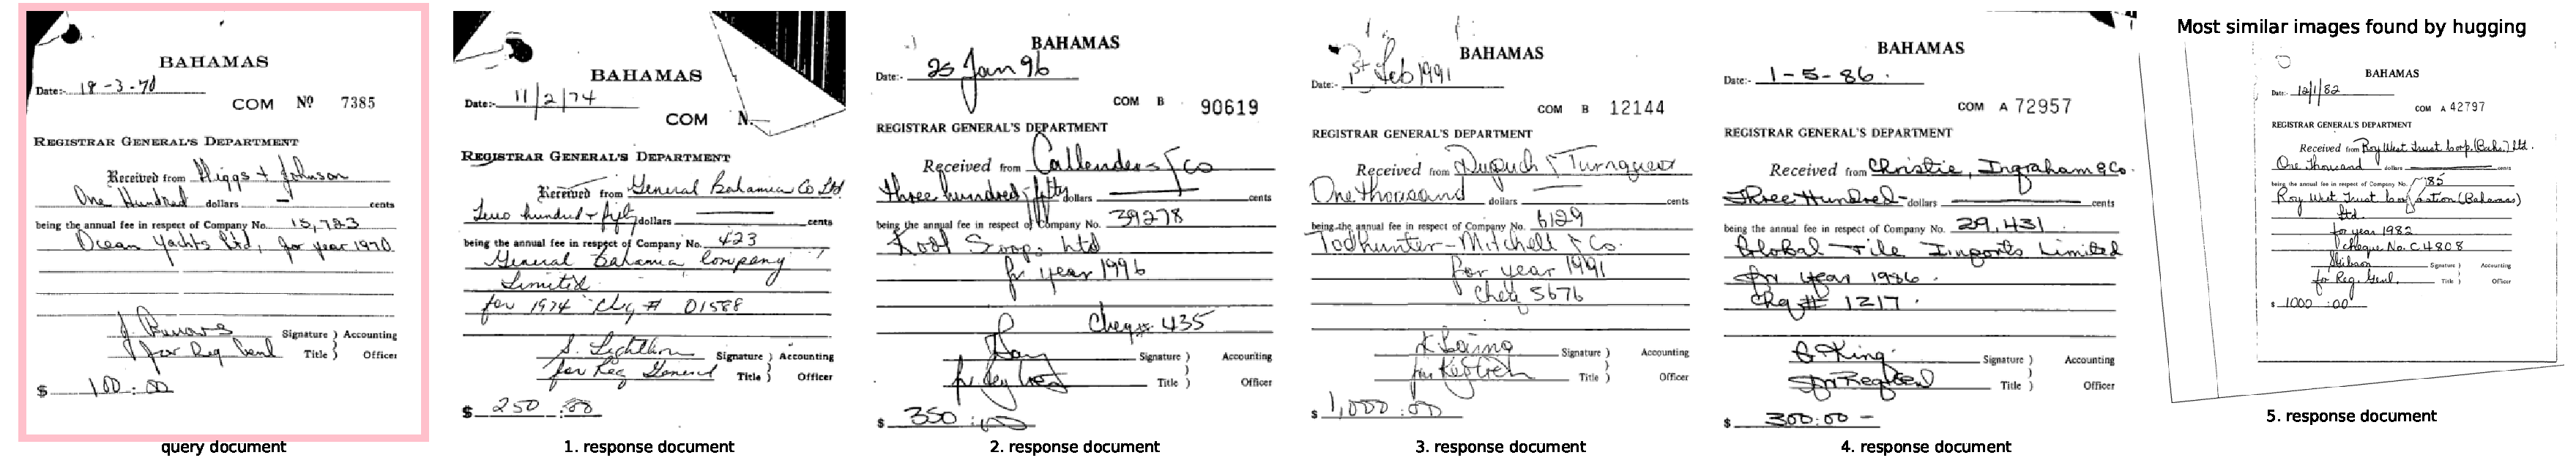
\includegraphics[width=1\textwidth]{images/query_results/4542b223317eba23e4bda3e1536d61c8e2d2890a6439830ca8c62650bc1aac70/Most_similar_images_found_by_hugging.pdf}
        \caption{\ac{sbert}}
        \label{fig:good_query_resp_sbert}
    \end{subfigure}

\caption[Qualitative comparison of query responses]{Qualitative comparison of query responses.
The majority of the query document consists of handwritten text.
The results of the \ac{tfidf} model are not very similar to the query document and thus, are considered to be of poor quality.
The other models, for example \ac{sbert}, produce results which are more similar to the query document.
}
\label{fig:comp_query_resp}
\end{figure}



% investigate certain images
any images which produce unusual results?

\section{Comparison with baseline topic analysis approach}\label{sec:evaluation-top-model-app}

The baseline topic analysis \ac{t2v} offers a variety of built-in functionalities to the user.
It is possible to retrieve human interpretable inherent topics of a set of documents, 
as well as the topics most similar to certain search terms 
and \wordcloud{}s of these results.
Hence, this library meets the needs articulated by this work.

% > 1 embedding model
Opposed to \ac{t2v}, this thesis proposes a composite of different approaches to encoding visual and semantic information 
and query for them using a database and visualization by the means of \wordcloud{}s.
To be more specific, this thesis not only relies on one semantic embedding model but offers several techniques and an approach to incorporate visual information.

% no topics for search terms
However, it is not possible to query for topics of the corpus which best describe a search term.
Alternatively, one can perform a fuzzy text search on the documents.
The user can inspect the \ac{pdf} of a document upon clicking on its name in the list of documents.
The detail component enables the investigation of similar documents in terms of different embedding approaches.

% topic definition
Due to \ac{t2v}'s architecture, documents and words are mapped into the same \ac{vsm}.
Hence, the topic vector definition and representation by its closest words are more meaningful than the approach of the thesis. 
In this thesis, a topic is represented by frequent words in the set of documents that are not necessarily meaningful. 

% term frequency
The tool implemented in this thesis can display the term frequency of the document chosen in the detail component.
The \ac{t2v} library does not offer a comparable service.
    \chapter{Conclusion \& Outlook}\label{ch:conclusion-outlook}

In the following, the results of this work are summarized and evaluated.
In \autoref{sec:conclusion} a discussion on the methods used and the contributions are presented.
This section focuses on the reason for choosing the methods and the way they are combined in this work.
It is stated why the bundle of techniques is of scientific interest.
\autoref{sec:outlook} concludes with an outlook on the shortcomings of this thesis and future work.

\section{Conclusion}\label{sec:conclusion}

The techniques examined in this work are discussed in \autoref{subsec:discussion}.
This section gives a brief outline for which reasons the techniques have been chosen.
Afterwards, the contributions of this work are summarized in \autoref{subsec:contribution}.


\subsection{Discussion}\label{subsec:discussion}

% preprocessing -> filter information
Before working with a model, the data has to be processed to a format that the model can work with.
The requirements imposed on the data format depend on the model.
Some models do not require any preprocessing, while others require a lot of preprocessing.

% tfidf preprocessing
Opposed to the other semantic embedding methods \ac{tfidf} requires preprocessing.
In this work, the \ac{tfidf} configuration includes the definition of a custom preprocessor.
Consequently, preprocessing plays an important role in this embedding.
The preprocessor is constructed with respect to the well-established preprocessing steps for \ac{nlp} tasks \cite{nlp-book2009},
the \ac{tfidf} documentation about the default preprocessor and the task.
Since the data set can contain figures due to the financial background, the preprocessor encodes all numbers into discrete strings.
Hence, the information is not lost but strongly reduced, which is vital due to the constraints imposed 
by the database's dense vector dimension limitation.
The custom preprocessor is compared to the default preprocessor on multiple datasets.
Since it consistently produces smaller vocabulary sizes, it is chosen for the task.

% visual preprocessing
The visual embedding methods also require preprocessing.
Originally, the images were matrices of \texttt{RGB} values.
However, \ac{pca} and \ac{optics} require a vector as input.
Therefore, the images are converted to greyscale and flattened to a vector.
The images are resized to make them more comparable.
Since clustering algorithms such as \ac{optics} encounter difficulties on high-dimensional data, 
applying \ac{pca} to compress the data can be considered preprocessing.


% compression: AE, PCA/ Eigendocs
As mentioned before, the database has a dense vector dimension limitation of 2048.
This limitation is a problem for the visual embedding methods as well as for \infersent{} and 
\ac{tfidf}.
The visual embedding methods are compressed with \ac{pca}, 
whereas the encoder of a trained \ac{ae} is employed for textual embeddings.
The \ac{pca} is fitted on 1000 randomly selected images.
The number of components is selected beforehand in consideration of the explained variance and the reconstruction error.
The architecture of the \ac{ae} is chosen in consideration of the reconstruction error on 195 documents.
However, both the \ac{pca} and the \ac{ae} model's quality would improve if they were trained on a larger dataset.


% visual vs semantic
As already stated this work examined both ways to encode semantic and visual information.
The evaluation is conducted with respect to the task of finding similar documents.
Since the data set is not labeled the evaluation is subjective and experimental.
Qualitative evaluation is conducted by inspecting the responses of different models for several sample queries to the database 
storing the respective embeddings.
The inspection is conducted manually, 
using Venn diagrams, heatmaps and 
statistical properties of the distribution of the cardinality of the shared query response sets.

The semantic responses are similar and often managed to find either documents with the same content or documents with the same company name.
The visual responses are more dissimilar from each other and the query document.
% visual: OPTICS, argmax
More precisely, the \texttt{argmax} approach returns poor results to some extent.
Consequently, \ac{optics} is considered the superior visual embedding method for the database.
Moreover, the textual embedding methods produce more meaningful responses than the visual embedding methods.
For example, textual embedding methods manage to find documents with the same company name, 
while visual embedding methods naturally return visually similar documents which not necessarily originated by the same company.


% semantic: TFIDF, Doc2Vec, USE, InferSent, SBERT
When evaluating the semantic embedding methods, slight differences between the models become evident.
Differences and similarities between the models are examined by comparing the responses to the sample queries.
This evaluation includes the calculation of the average portion of shared documents between the responses of several models 
and the exemplary evaluation of actual queries.
\ac{tfidf}, \ac{d2v} and \ac{sbert} are most dissimilar from each other.
The \ac{tfidf} approach performs rather poorly on unusual query documents such as handwritten documents.


% similarity: cosine
The similarity metric used in this work is cosine similarity.
Since \databaseName{} provides the similarity metrics Euclidean distance, dot product and cosine similarity,
one of these metrics had to be chosen.
Usually, cosine similarity is recommended for \ac{nlp} tasks and thus, applied in this work.
Soft cosine similarity is not used, since it is not available in \databaseName{}.
However, the usage of soft cosine would likely improve the results.

% topic analysis: wordclouds
Since the techniques discussed in this section have to be merged into a single system 
\wordcloud{} provides means to visualize the response documents containing the most similar documents for different models.
This approach is well suited to describe topics as groups of predominant words \cite{topic_modeling2019}.
The baseline topic analysis technique \ac{t2v} provides a \wordcloud{} implementation too.

% database: Elasticsearch
The database used in this work is \databaseName{}.
It was built to provide a fast and scalable search engine.
Moreover, it is a document-oriented database, which is well-suited for flexible data.
By default, several similarity measures and search strategies are provided.
Moreover, the elastic stack offers a wide range of tools supporting embedding models which are not used in this work.


% FE (Angular), BE (Flask)
The libraries used for the implementation of the tool are \angular{} and \flask{}.
The libraries were chosen after discussing options with this thesis' supervisor.
However, the implementation of this tool is not the focus of this work.

% top2vec
The baseline topic analysis technique \ac{t2v} is chosen due to its simplicity and functionalities.
The \ac{t2v} implementation is well documented and provides a \wordcloud{} implementation.
Moreover, it enables the user to find similar topics for query terms and returns inherent topics in a data corpus.
Hence, its functionality is similar to the functionality of the system developed in this work.

\subsection{Contribution}\label{subsec:contribution}
% mein Beitrag
% literature review, semantic -> visual
An exhaustive literature review was conducted to find suitable embedding methods for the task of finding similar documents.
Initially, only semantic embedding methods were considered.
However, when the first results were inspected the idea arose to group the documents by visual similarity.
Thus, visual embedding methods were included in the evaluation.

% using existing models
The semantic embedding methods were implemented using existing models.
All models offer adequate documentation and were thus, mostly comfortable to use.
However, some alterations had to be made to the models to make them suitable for the task.
For instance, a custom preprocessor was implemented for the \ac{tfidf} embedding method.
The preprocessor was a better fit for the task than the default preprocessor.
Moreover, a custom \ac{w2v} model was trained on the data set to be used by \infersent{}.
This reduced the time necessary to encode texts.

% eigenfaces -> eigendocs
The \eigenfaces{} approach has been prevalent since \citeyear{eigenfaces1991}.
In this work, the approach was adapted to the task of finding similar documents and thus, called \eigendocs{}.
The idea of projection items into a lower dimensional space was kept as well as the preprocessing steps.
However, the preprocessing was extended by placing the document images onto a white canvas.


% clustering
In order to find a suitable clustering algorithm for the task, literature research was conducted.
The research revealed that the \ac{optics} algorithm is a suitable candidate for the task.
In this work, two different preprocessing steps were implemented.
The first was similar to the preprocessing steps used in \cite{OPTICS1999}.
The second one utilized \eigendocs{} to reduce the dimensionality of the data set.
The parameters of the algorithm were chose in consideration of the reachability plot.


% pca components/ AE architecture evaluation
The data was compressed using \ac{pca} or the encoder of an \ac{ae}.
Both the \ac{pca} and \ac{ae} configurations were experimentally evaluated.
The number of components of the \ac{pca} was chosen in consideration of the cumulative explained variance 
and the reconstruction error.
The architecture of the \ac{ae} was chosen in consideration of the reconstruction error \ac{rsme} and 
the cosine similarity between the original and the reconstructed vector.


% database local & server
Before the data could be used for the task, it had to be stored in a database.
Firstly, the type of database had to be chosen.
It became clear that a document database would be the best fit for the task 
since it accepts documents of variable shape.
\databaseName{} is a well-known document database that is used by 
well-established companies successfully handling big data.
Secondly, the database had to be configured.
This required the consideration of different field types and similarity measures.
The dense vector seemed to be a native choice and cosine similarity was chosen 
among other reasons due to its popularity as a similarity metric in \ac{vsm}.
Afterwards scripts to store the data in the database were implemented.
The local database stores 2048 randomly chosen documents from the whole data set.
The server database currently stores around $497504$ incomplete documents.

% evaluation: venn & heatmap, mean/ std
Since the dataset is not labeled, the evaluation of the results is not trivial.
Therefore, multiple evaluation methods were implemented.
The first method is a Venn diagram that shows the intersection of the results of the power set of different methods.
The second method is a heatmap that shows the average portion of shared response documents between different methods.
Lastly, the mean and standard deviation of the portion of shared response documents were calculated 
to further investigate the distribution of the results obtained above.

% topic modeling
To ensure \wordcloud{}s display only valid words the tokens were lemmatized before applying the \wordcloud{}. 
The existing functionalities implemented by the library \topTwovec{} were bundled into a class 
which accepts inputs native to the task at hand.
Hence, the functionalities were not extended but rather adapted to the task.  


% chapter about motivation -> goals, techniques used and COMBINED
As initially mentioned, this thesis aims to provide computational means to facilitate the work with large unstructured text data.
In the course of this work, multiple \ac{ml} techniques were examined and evaluated on the task of finding similar documents.
The semantic embedding methods \ac{tfidf}, \ac{d2v}, \infersent{}, \ac{use} and \ac{sbert} were examined.
\eigendocs{} was implemented as a visual embedding method.
It was possible to find a suitable database to store the data.
A pipeline to preprocess, embed and store the data in the database was developed.
The pipeline is scalable to large datasets.
However, models such as \ac{tfidf} yield less meaningful results on certain query documents and 
are prone to performance deterioation with increasing document corpus, since the embeddings' 
dimensionality correlates directly with the vocabulary size.
When the number of terms in the data corpus increases, but the vocabulary size is static, 
it is likely that the vocabulary lacks important words. 

Moreover, a tool was implemented.
The tool provides the possibility to conduct text queries.
A document of interest can be examined in more detail:
The detail component not only contains a \ac{pdf} viewer, 
a \wordcloud{} of the most frequent words in the document, but also an option to examine the query responses for different embeddings.
The file names of the ten most similar documents and a \wordcloud{} of the most frequent words among those documents is displayed.

An experimental evaluation of the embeddings was conducted.
The visual embedding methods were found to be inferior to the semantic embedding methods on certain query documents.
The tool was compared to a baseline topic modeling approach called \topTwovec{}.
The library \topTwovec{} implemented similar functionalities.
However, the tool is not designed for a productive environment since the focus is on the comparison of different models rather than usability.


\section{Outlook}\label{sec:outlook}
% features of the application

% What did I find?
When investigating both semantic and visual embedding methods, differences between the models became evident.
Overall, the textual embedding methods produced more meaningful responses than the visual embedding methods.
However, this is not surprising since the textual embedding methods prioritize documents containing equal or semantically similar terms and thus,
return documents of similar content or originating from the same company as the query document.
Visual embedding methods, on the other hand, return visually similar documents.

It is complicated to compare the responses of semantic and visual embedding methods since they operate on fundamentally different data.
A more thorough evaluation could include a survey.
A selection of the results of this work is incorporated into the first approach to constructing a survey.
13 people with different academic backgrounds have partaken in the survey.
A question and result from the survey are displayed in \autoref{fig:survey}.
However, constructing a survey is complicated since semantic similarities should be evaluated on a textual level, i. e. content, 
which is difficult for non-experts and not natural since humans are prone to assess similarities by visual inspection.
Moreover, identification of the target audience is difficult since the target audience of the tool could be expanded to be more general than the tax office.

\begin{figure}%
    \centering
    \subfloat[\centering A question of the survey.]{{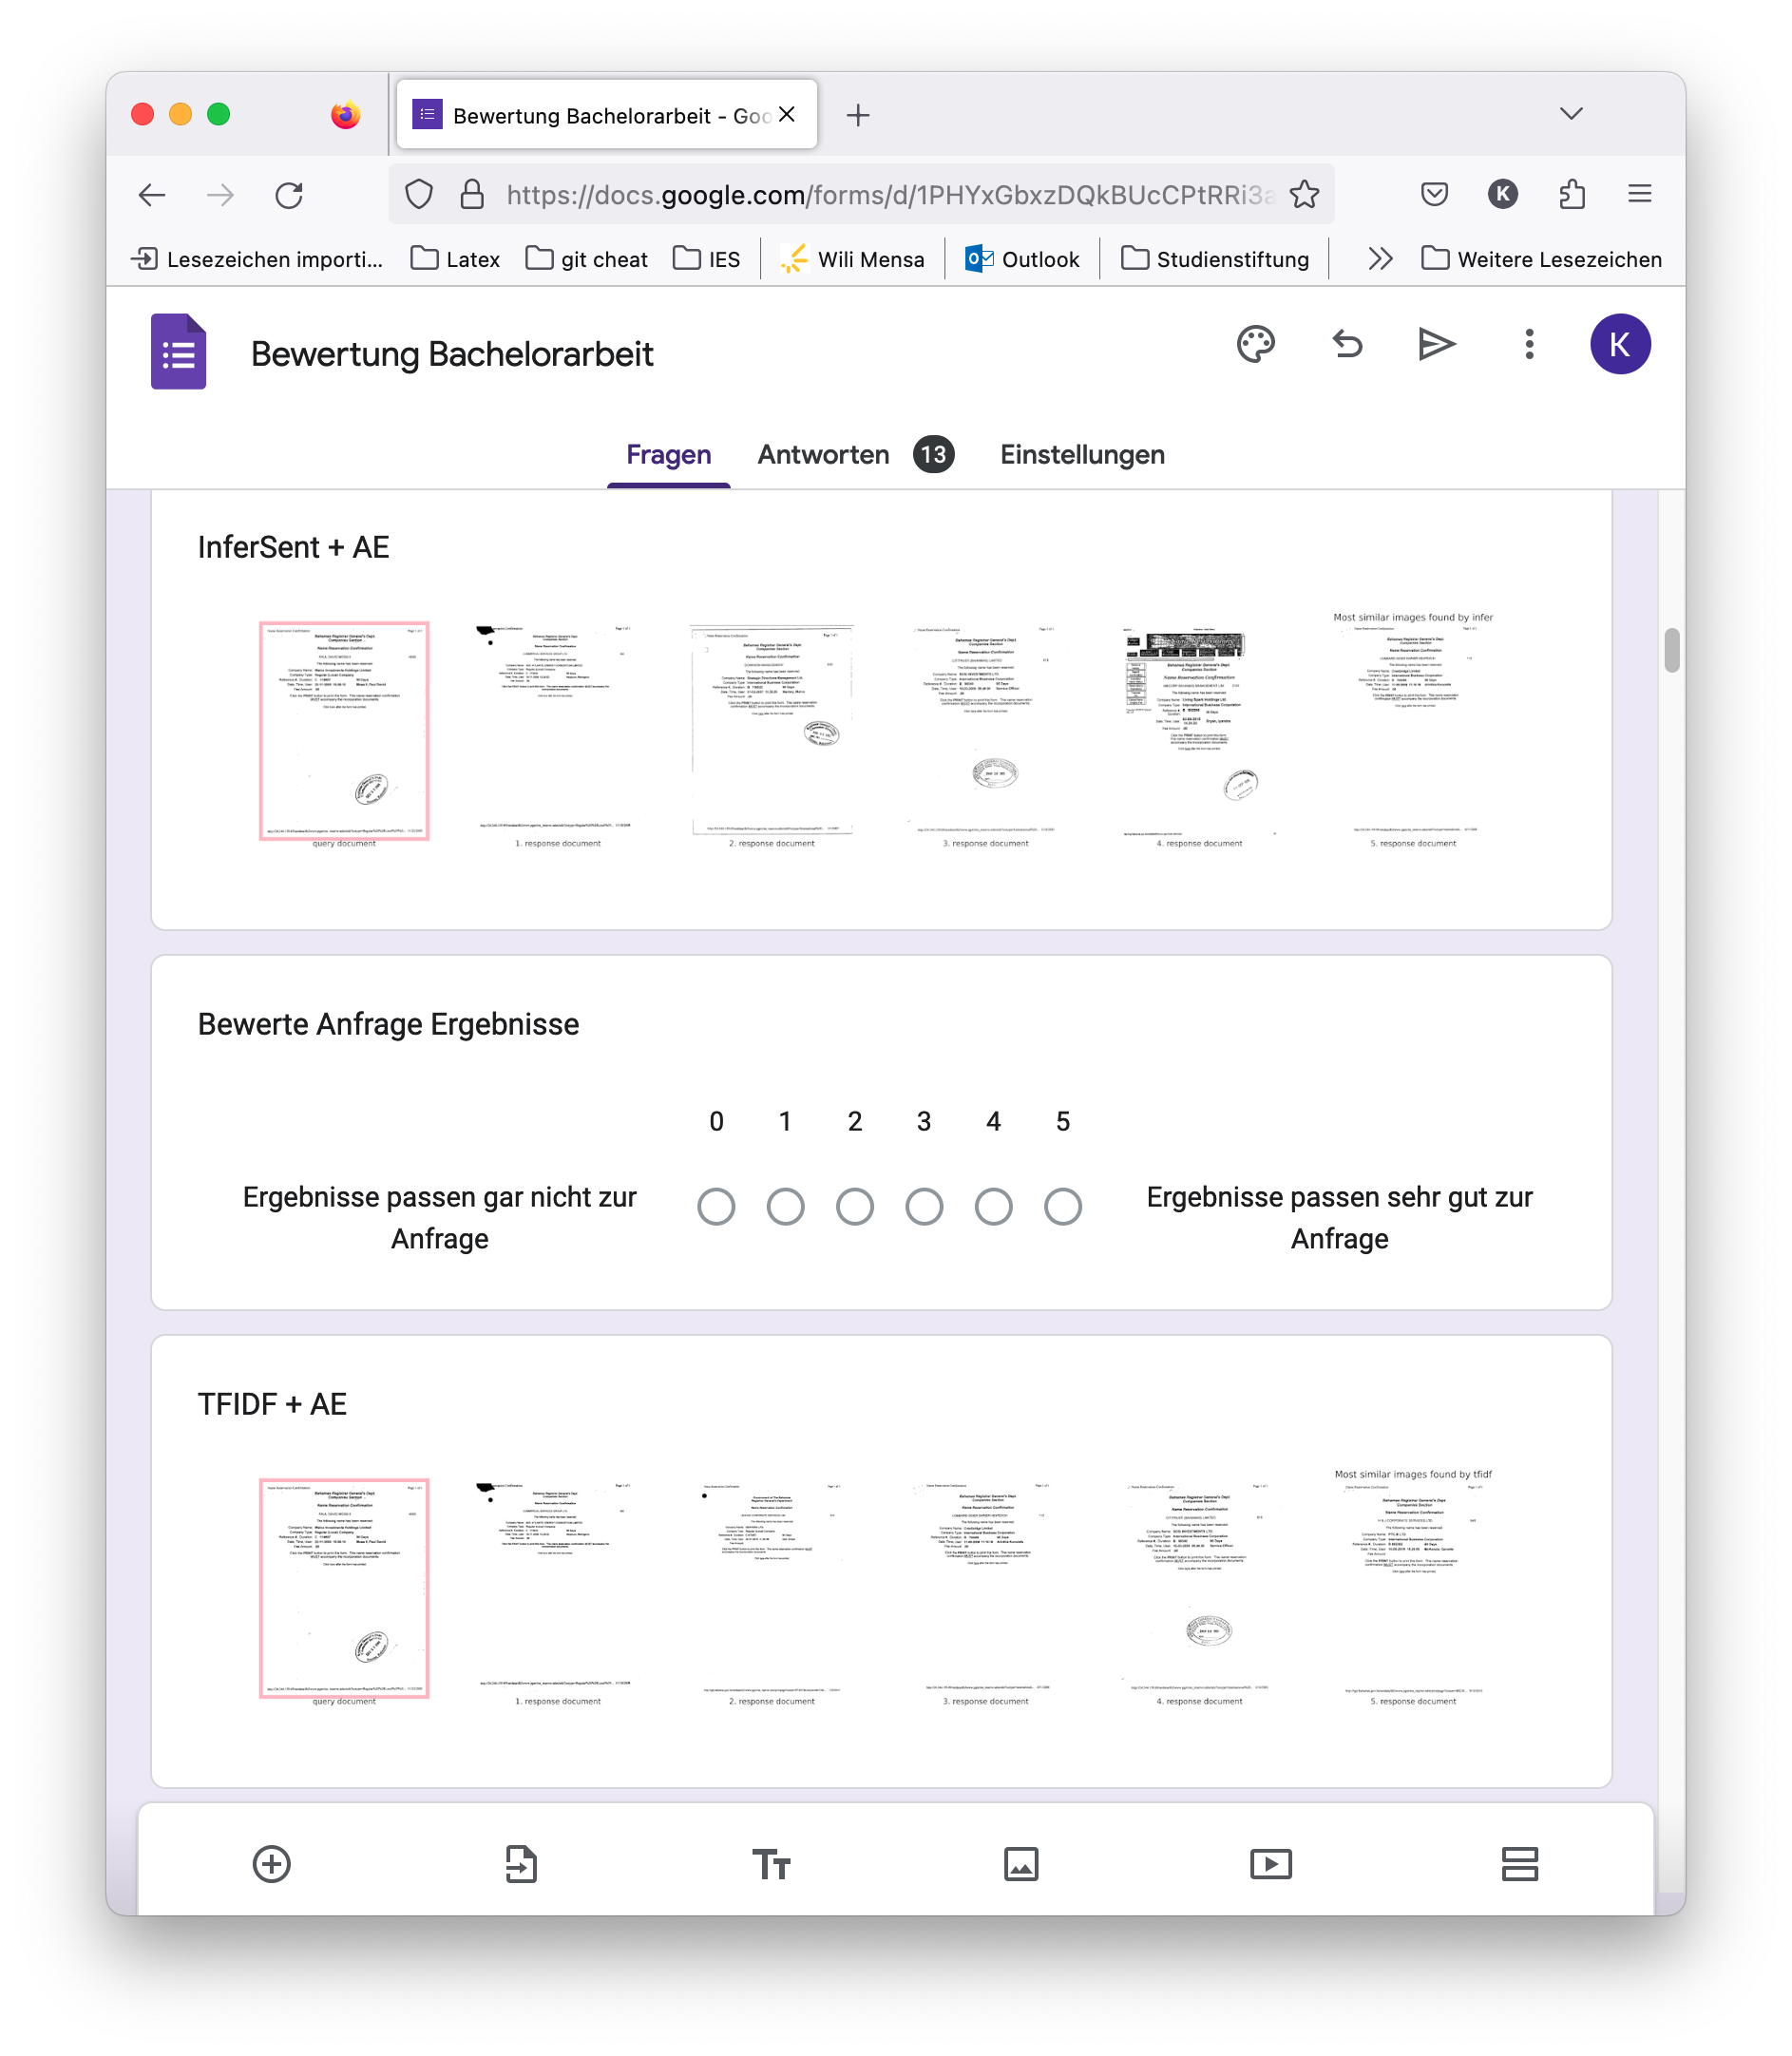
\includegraphics[width=5cm]{images/Umfrage/Umfrage_ex.png} }}%
    \qquad
    \subfloat[\centering Selection of results of survey.]{{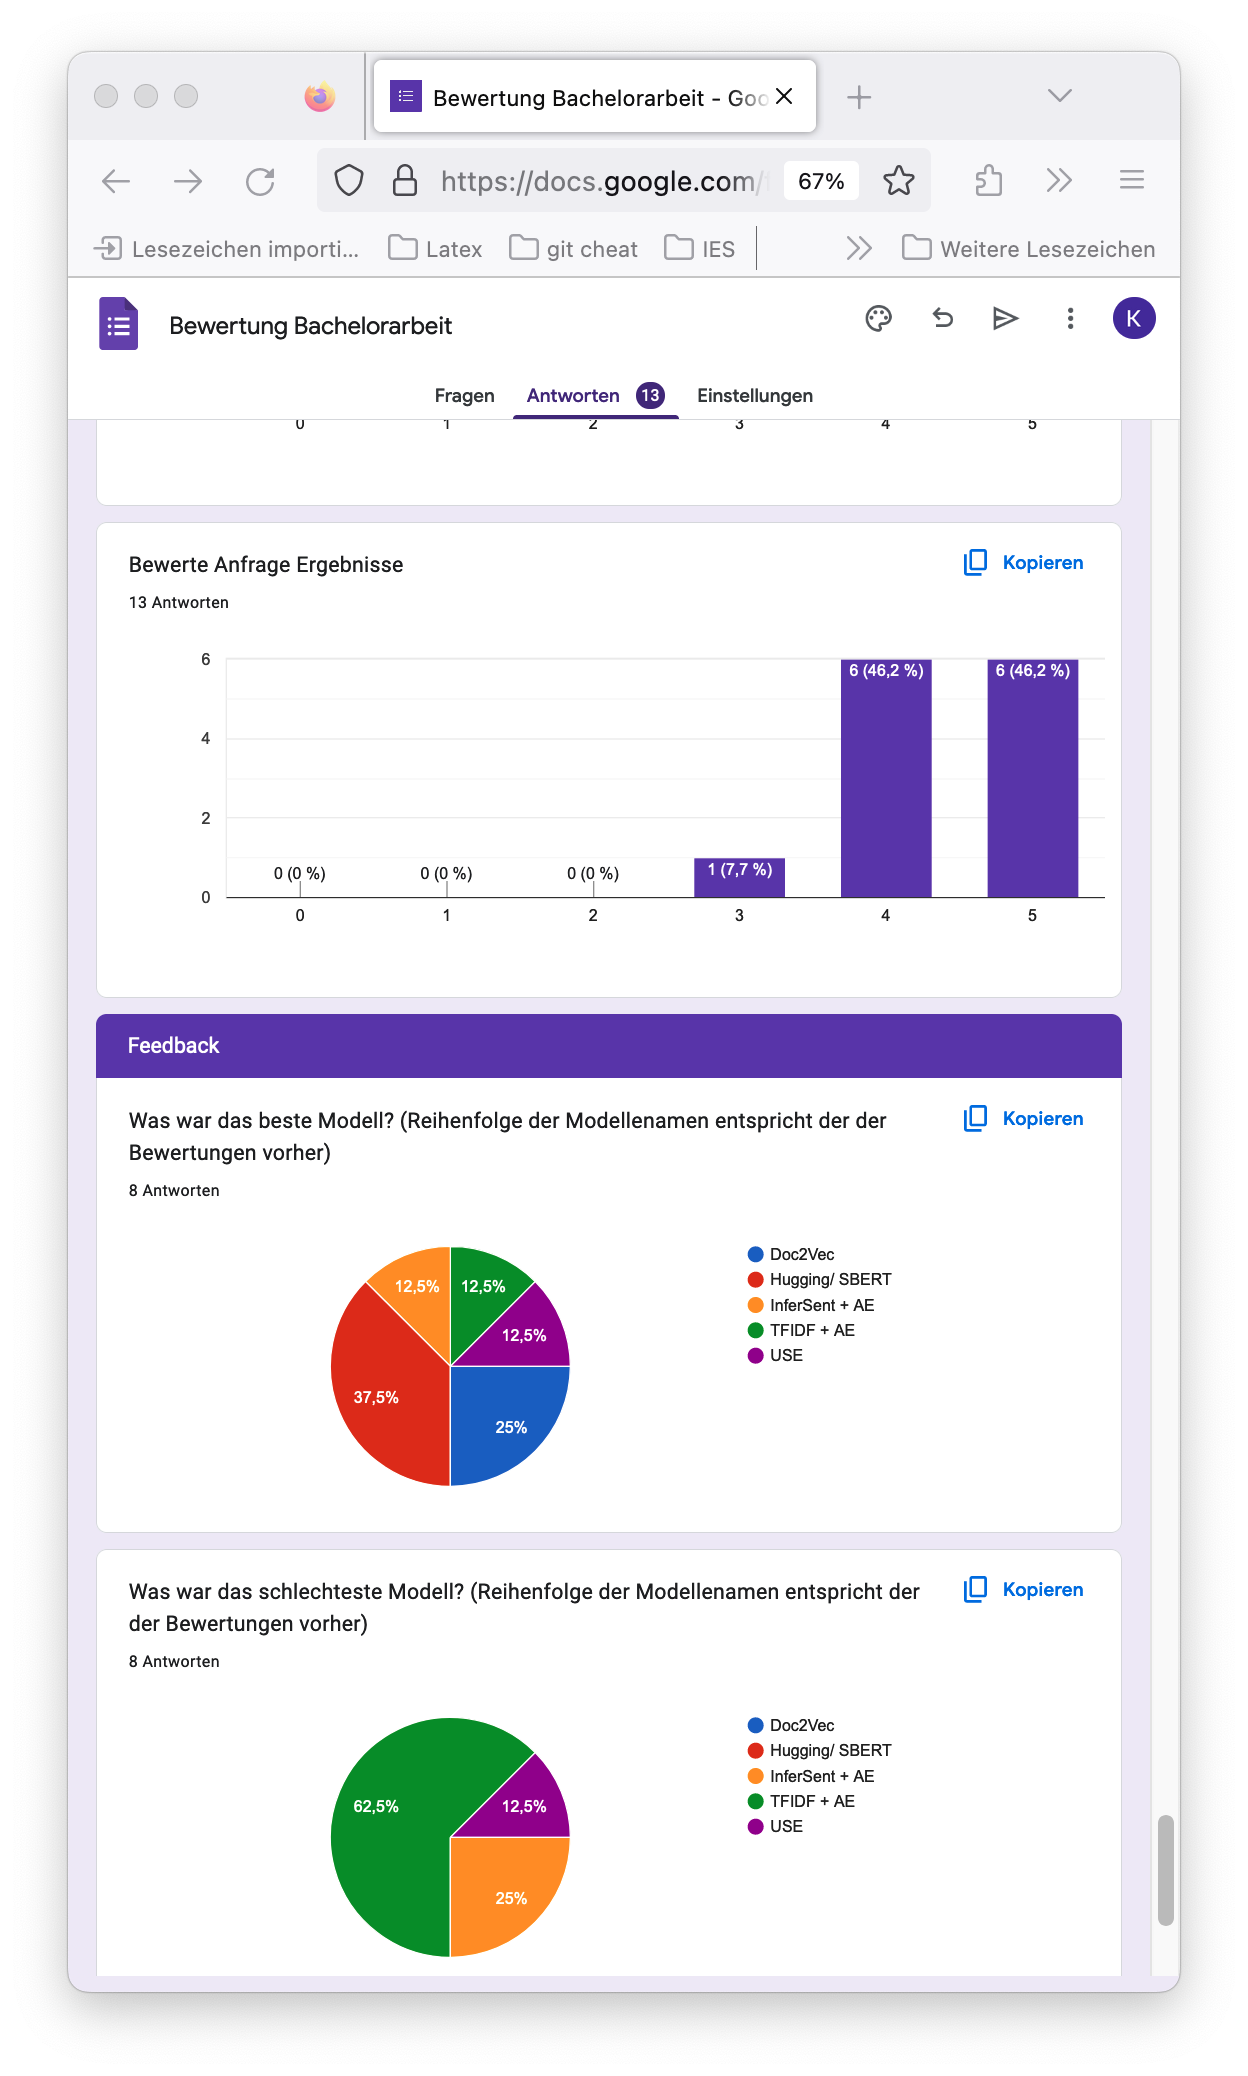
\includegraphics[width=5cm]{images/Umfrage/Umfrage_erg.png} }}%
    \caption[Survey approach]{A first survey approach from \cite{BA-survey}.}%
    \label{fig:survey}%
\end{figure}

% Problems/ critic
% Embedding methods
% hyperparameter tuning
Similar to \citeauthor{glove2014}'s work, in this thesis, for many models used, any unspecified parameters are set to their default values, 
assuming that they are close to optimal
acknowledging that this simplification should be revised in a more thorough analysis.

% TFIDF
The \ac{tfidf} approach performs rather poorly on unusual query documents.
There are multiple factors that could have contributed to this result.
Firstly, the vocabulary is drastically reduced to satisfy the database's constraints for dense vector dimensionality.
Thus, \ac{tfidf} may either be unsuitable for the task of finding similar documents when the vocabulary size is restricted or 
further research is required to find more suitable means to compress the embedding before inserting it into the database.
Secondly, the evaluation of the different preprocessors of \ac{tfidf} is carried out on small datasets of 195 and 2048 documents.
This dataset may not be representative of the whole corpus.

% GloVe (InferSent)
In this work, the precomputed \ac{glove} embeddings are replaced by a custom \ac{w2v} model.
However, \citeauthor{glove2014} state that \acs{glove} outperforms \ac{w2v} on the same corpus, 
vocabulary and window size in terms of quality \cite{glove2014}.
Hence, the quality of \infersent{} might have deteriorated due to the replacement of \ac{glove} by \ac{w2v}.

% Visual embedding methods
% Eigendocs
When preprocessing the document images for \eigendocs{}, the images are placed on a white canvas assuming 
its dimensions are bigger or equal to all other documents in the corpus.
Since this assumption was not true, the images selected to find the dimensionalities of the canvas are not representative.

% compression: PCA
The parameter selection for \ac{pca} is not representative of the whole dataset, 
due to the fact that the dataset used for the evaluation error was not drawn randomly from the data corpus and is too small.
Moreover, the resulting plot is not optimal for conducting the "elbow method", since no significant change is evident in the slope.


% AE config: Problem & future work
Different \ac{ae} architectures are experimentally evaluated on a selection of 195 documents.
However, since the dataset is too small and not drawn randomly from the whole data corpus the results are not representative.
Thus, future work should include a more thorough evaluation of different \ac{ae} architectures on a bigger document corpus.
% tfidf + AE only used on server

% comparison on training data
The comparison of the different embedding methods in terms of query response similarity was carried out on the data which was stored in the database.
For future work, the comparison should be carried out on a separate data set to evaluate the performance of the models on unseen data.

% eval weights of response documents
The evaluation of the similarity between query results of different models so far 
has not considered the individual weights for respective query responses
because it was difficult to find means 
to interpret and visualize semantic meaningful weight relationships.
Thus, future work could include the weights of the query responses in the evaluation.

% similarity of query documents
Moreover, the similarity of the query documents is not considered in the evaluation.
To further improve the evaluation, the number of occurrences of query documents in the response documents of other queries could be examined.

% elastic stack: Kibana
The elastic stack offers a wide range of tools, for instance, Kibana that can be used to manage models and 
to create ingest pipelines to embed new documents.
If models are managed by Kibana, the models no longer have to be managed by the user and thus, 
the system would most likely be more user-friendly and less prone to errors.

% server database
Another issue is the fact that the database contains neither all embeddings nor all documents.
The Bahamas leak contains 38 \ac{gb} of data.
Even though multiprocessing using Pool is used to split the workload across up to 100 processes, 
the embedding process is not finished after several days.
Hence, more advanced coding techniques have to be applied to speed up the embedding process.

% Future: continue developing this application with the tax office
The domain of financial fraud and tax evasion is very interesting.
Thus, future work could include the development of a working system for the tax office.
The techniques explored in this work could be used to find similar documents to a query document and thus,
facilitate initial exploration of a large data corpus.
However, the tool developed in this work is not yet ready to be used in tax offices.
The different embedding models to choose from are useful for research purposes but not in a productive environment.


    % Die nächsten zwei Zeilen sind optional, sie sorgen dafür dass alles nach dem Inhalt wieder mit römischen Zahlen nummeriert wird.
    \pagenumbering{roman}
    \addtocounter{page}{4} % Dies ist die Anzahl der Seiten vor der Einleitung, muss möglicherweise angepasst werden, wenn das Inhaltsverzeichnis mehrere Seiten umfasst.

    \bibliography{
        bibliography/information-retrieval,
        bibliography/data-corpus,
        bibliography/embeddings,
        bibliography/database,
        bibliography/slurm,
        bibliography/clustering,
        bibliography/eigenfaces,
        bibliography/user_interface,
        bibliography/similarity,
        bibliography/autoencoder,
        bibliography/topic_modelling,
        bibliography/financial_dataset
    }

    \chapter*{Declaration of authorship}

% Inhaltsverzeichnis und Kopfzeile
% \addcontentsline{toc}{chapter}{Eidesstattliche Erklärung}
\markboth{Declaration of authorship}{Declaration of authorship}

I hereby declare that I am the sole author of the bachelor’s thesis with the title "\thesistitle" 
and that I have not used any sources other than those listed in the bibliography and identified as references. 
I further declare that I have not submitted this thesis at any other institution in order to obtain a degree.

\vspace{1cm}

Kassel, \thesisdate

\begin{flushright}
  \underline{\hspace{7cm}} \\
  \thesisauthorname
\end{flushright}

\end{document}
